\documentclass{book}
\usepackage[gen]{eurosym}
\usepackage[spanish]{babel}
\usepackage{amsmath}
\usepackage{graphicx}
\usepackage{subfigure}
\usepackage{listings}
\usepackage{tikz}
\usepackage{circuitikz}
\usetikzlibrary{babel}
\usepackage{array}
\usepackage{makecell}
\usepackage{tabularray}
\usepackage{subcaption}
\usepackage{booktabs}
\usepackage{siunitx}
\usepackage{pgfplots}
\usepackage{pgfplotstable}
\usepgfplotslibrary{colormaps}
\pgfplotsset{compat=1.17}
\usepgfplotslibrary{groupplots}
\usepackage{pdflscape}
\usepackage{amssymb}

\usepackage{multicol}
\usepackage{multirow}
\usepackage{float}
\usepackage{xcolor}
\usepackage{pgf-pie}
\usepackage{pgffor}
\usetikzlibrary{arrows}
\usepackage{titlesec}
\usepackage[T1]{fontenc}
\usepackage{tgpagella}
\usepackage{amsmath}
\usepackage[a4paper, top=2cm, bottom=2cm, left=3cm, right=3cm, marginparwidth = 1.75cm]{geometry}

\graphicspath{ {./res/tema1/} }

\setlength\parindent{12pt}

\title{Apuntes de Diseño de Centrales Eléctricas}
\author{Bogurad Barañski Barañska \and Adrián Teixeira de Uña}
\date{\today}

\def\innerradius{3cm}
\def\outerradius{4cm}
\newcommand{\grado}{°C}

% Macro principal para el gráfico de donut
\newcommand{\donutchart}[1]{
	% Calcula el total
	\pgfmathsetmacro{\totalnum}{0}
	\foreach \value/\colour/\name in {#1} {
		\pgfmathparse{\value + \totalnum}
		\global\let\totalnum=\pgfmathresult
	}
	
	\begin{tikzpicture}
		% Calcula el grosor y la línea media del gráfico
		\pgfmathsetmacro{\wheelwidth}{\outerradius - \innerradius}
		\pgfmathsetmacro{\midradius}{(\outerradius + \innerradius) / 2}
		
		% Gira el gráfico para comenzar desde la parte superior
		\begin{scope}[rotate=90]
			% Bucle a través de cada conjunto de valores
			\pgfmathsetmacro{\cumnum}{0}
			\foreach \value/\colour/\name in {#1} {
				\pgfmathsetmacro{\newcumnum}{\cumnum + \value / \totalnum * 360}
				% Calcula el valor porcentual
				\pgfmathsetmacro{\percentage}{\value / \totalnum * 100}
				% Calcula el ángulo medio de los segmentos de color para colocar las etiquetas
				\pgfmathsetmacro{\midangle}{-(\cumnum + \newcumnum) / 2}
				% Esto es necesario para que las etiquetas se alineen correctamente
				\pgfmathparse{(-\midangle < 180 ? "west" : "east")}
				\edef\textanchor{\pgfmathresult}
				\pgfmathsetmacro\labelshiftdir{1 - 1 * (-\midangle > 180)}
				% Dibuja los segmentos de color
				\fill[\colour] (-\cumnum:\outerradius) arc (-\cumnum:-(\newcumnum):\outerradius) -- (-\newcumnum:\innerradius) arc (-\newcumnum:-(\cumnum):\innerradius) -- cycle;
				% Establece el ángulo acumulado antiguo al nuevo valor
				\global\let\cumnum=\newcumnum
			}
		\end{scope}
	\end{tikzpicture}
}

\begin{document}
\frontmatter	
	\mainmatter	
		\maketitle
		\tableofcontents
		\addcontentsline{toc}{chapter}{Índice}
		
\section{Tema 1: Introducción y generalidades sobre metrología}
\subsection{Definiciones}
\begin{enumerate}
	\item \underline{\textbf{Magnitud}}: 
	\item \underline{\textbf{Magnitud básica}}:
	\item \underline{\textbf{Magnitud derivada}}:
	\item \underline{\textbf{Unidad de medida}}:
	\item \underline{\textbf{Unidad coherente}}:
	\item \underline{\textbf{Sistema de unidades}}:
	\item \underline{\textbf{Valor de una magnitud}}:
	\item \underline{\textbf{Valor verdadero}}:
	\item \underline{\textbf{Valor convencionalmente verdadero}}:
	\item \underline{\textbf{Medida}}:
	\item \underline{\textbf{Medición general}}:
	\item \underline{\textbf{Medición metrológica}}:
	\item \underline{\textbf{Mensurando}}:
	\item \underline{\textbf{Magnitud de influencia}}:
	\item \underline{\textbf{Señal de medida}}:
	\item \underline{\textbf{Instrumento de medida}}:
	\item \underline{\textbf{Cadena de medida}}:
	\item \underline{\textbf{Valor nominal}}:
	\item \underline{\textbf{Campo de medida}}:
	\item \underline{\textbf{Rango de medida}}:
	\item \underline{\textbf{Constante de medida}}:
	\item \underline{\textbf{Estabilidad}}:
	\item \underline{\textbf{Transparencia}}:
	\item \underline{\textbf{Deriva}}:
	\item \underline{\textbf{Zona muerta}}:
	\item \underline{\textbf{Sensibilidad}}:
	\item \underline{\textbf{Resolución}}:
	\item \underline{\textbf{Veracidad}}:
	\item \underline{\textbf{Precisión}}:
	\item \underline{\textbf{Exactitud}}:
	\item \underline{\textbf{Sesgo}}:
	\item \underline{\textbf{Linealidad}}:
	\item \underline{\textbf{Índice de clase}}:
	\item \underline{\textbf{Incertidumbre de medida}}:
	\item \underline{\textbf{Error de medida }}:
	\item \underline{\textbf{Error aleatorio}}:
	\item \underline{\textbf{Error sistemático}}:
	\item \underline{\textbf{Tolerancia}}:
	\item \underline{\textbf{Incertidumbre}}:
\end{enumerate}
\subsection{Causas de errores}
\subsection{Ley propagación de incertidumbres}
\subsection{Estimación de la incertidumbre}
\subsection{Relación tolerancia incertidumbre}
\subsection{Relación incertidumbre resolución}
		\chapter{Energía eléctrica y desarrollo sostenible.}

\section{Introducción al desarrollo sostenible.}
El desarrollo nació en los años 70 en los países nórdicos y se define como:
\begin{itemize}
	\item [-] El que satisface
	nuestras necesidades actuales sin poner en peligro la
	capacidad de las generaciones futuras para satisfacer sus
	propias necesidades abarcando:
	\begin{itemize}
		\item El capital social
		\item El capital ambiental
		\item El capital económico
	\end{itemize}
\end{itemize}
\subsection{Cumbres climáticas.}
\begin{itemize}
	\item [-] \textbf{Rio de Janeiro (1992):}
		Se crea la Comisión del Desarrollo Sostenible para impulsar la sostenibilidad de las políticas de desarrollo humano y gestionar sus riesgos.
	\item [-] \textbf{Cumbre del Protocolo de Kyoto (1997):}
		Se adquiere un compromiso entre los países industrializados con el \textbf{objetivo} de reducir las emisiones de gases de efecto invernadero un 5,9\% en el periodo 2008 - 2012 con respecto a 1990 (año base). En una fase inicial no incluía a países en desarrollo como China e India por su baja contaminación per capita.
	\item [-] \textbf{Cumbre de París (2015):}
		Se comprometen los países a que la temperatura mundial no aumente más de 2\textdegree C respecto a los niveles preindustriales y limitarlo a 1,5\textdegree C para el 2020.
	\item [-] \textbf{Cumbre de Marrakech (2016):}
		Se ratifican los acuerdos de la Cumbre de París y se compromete reducir el 80\% de las emisiones de CO$_2$ para 2050.
	\item [-] \textbf{Cumbre de Katowice (2018):}
		Limitar a un incremento a final de siglo de 1,5 a 2\textdegree C respecto a los niveles preindustriales.
	\item [-] \textbf{Cumbre de Chile celebrada en Madrid (2019):}
		Los grandes contaminadores se niegan a intensificar los esfuerzos para mantener la temperatura por debajo de 1,5\textdegree C.
	\item [-] \textbf{Cumbre de Glasgow (2021):}
		Se mantiene el objetivo de 1,5\textdegree C para 2030. Acuerdo China - USA para reducir las emisiones de metano. Compromiso de 130 países para poner fin a la deforestación.
	\item [-] \textbf{Cumbre de Sharm el-Sheij en Egipto (2022):}
		Se acuerdan:
		\begin{itemize}
			\item Una alianza global contra la sequía.
			\item Una coalición contra la deforestación.
			\item Impulsar el hidrógeno verde.
			\item Impulsar la energía eólica marina.
		\end{itemize}
	\item [-] \textbf{Cumbre de Dubai(2021):}
		Se acuerda reducir las emisiones mundiales de gases de efecto invernadero un 43\% hasta
		2030 y un 60\% hasta 2035 en relación con los niveles de 2019, y emisiones netas de dióxido de carbono cero
		para 2050.
\end{itemize}
\section{Gases de efecto invernadero.}
\subsection{CO$_2$ equivalente.}
Es una forma de poder reducir el impacto climático a una unidad común y así, poder compararlos. Para calcularlo se emplea el valor \textbf{GWP} (Global Warming Potencial) o \textbf{PCG} (Potencial de calentamiento global) que miden cuanto calor atrapan en comparación con el CO$_2$ para un periodo de tiempo. 


Este valor depende de:
\begin{itemize}
	\item [-] La absorción de radiación infrarroja.
	\item [-] La ubicación del espectro de absorción.
\end{itemize}
\subsection{Dióxido de carbono (CO$_2$).}
Es la sustancia que más contribuye al efecto invernadero. Absorbe gran parte de la radiación solar incidente.
\subsection{Óxido nitroso (N$_2$O) y óxidos de nitrógeno (NO$_x$ ).}
Son los gases de efecto invernadero más destructivos con la capa de ozono. Relacionados con el sector agrario y la quema de combustible.
\subsection{Metano (CH$_4$).}
Tiene un potencial de calentamiento muy elevado GWP = 25. Se emite por el sector ganadero, el de tratamiento de residuos y durante el transporte de hidrocarburos.
\subsection{Hidrofluorocarbonos (HFC).}
Son gases empleados como refrigerantes. No dañan al ozono pero tienen un GWP = 1000 y una larga permanencia en la atmósfera.
\subsection{Perfluororcarburos (PFC).}
Similares a los HFC.
\subsection{Hexafluoruro de azufre (SF$_6$).}
Se emplea para equipos de distribución de energía eléctrica. Tiene propiedades similares a los HFC y PFC.

\begin{table}[H]
	\centering
	\begin{tabular}{p{2cm}p{2cm}p{2cm}p{2cm}p{2cm}}
		\hline
		\textbf{ } & \textbf{CO$_2$} & \textbf{ClFCs} & \textbf{CH$_4$} & \textbf{N$_2$O} \\ \hline
		Importancia según contribución al efecto invernadero & Más del 50\% & 20 \% aprox. & 12 a 14 \% & 6 a 7 \% \\ \hline
		Tiempo de permanencia en la atmósfera & 50 - 200 años & 75 - 100 años & 7 a 10 años & 150 años aprox. \\ \hline
		Tasa de crecimiento anual (\%)&0,5&4-5&1&0,35\\ \hline 
		Principal origen de la contaminación&Combustión del petróleo, carbón y gas deforestación&Aerosoles y disolventes Espumas industriales Equipos de refrigeración&Pantanos Ganadería Minería&Fertilizantes Combustible fósiles\\ \hline 
	\end{tabular}
	\label{tab:my-table}
\end{table}

\section{Efecto invernadero.}
Como consecuencia de los gases de efecto invernadero se absorbe una mayor cantidad de radiación infrarroja que escaparía de la tierra y, por tanto, aumentando la temperatura atmosférica. 
\begin{figure}[H]
	\centering
	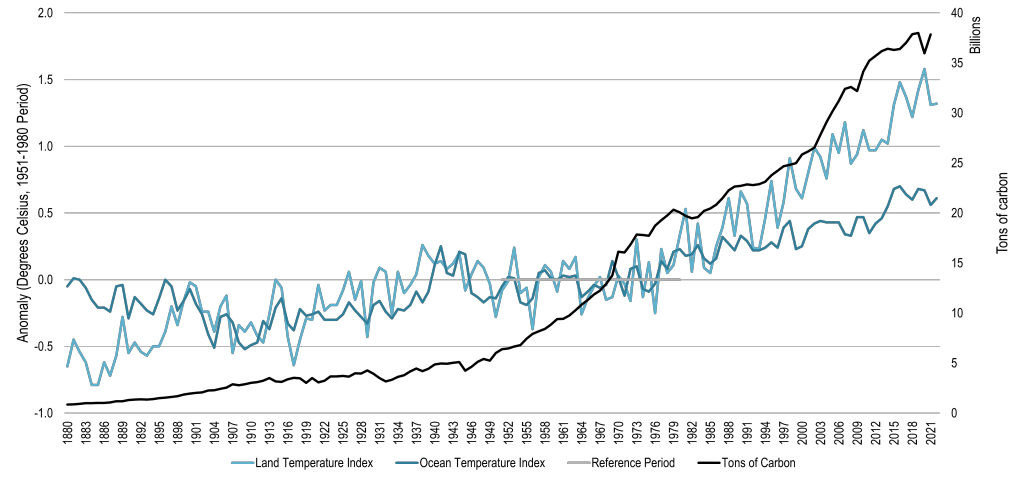
\includegraphics[width=0.7\linewidth]{res/tema2/T-Emisiones}
	\label{fig:t-emisiones}
\end{figure}
\subsection{Forzamiento radiactivo o climático.}
Es la diferencia entre la radiación solar absorbida por la Tierra y la energía irradiada de vuelta al espacio. Esta diferencia se contempla mediante el RCP donde:
\begin{itemize}
	\item [-] RCP = 2 es un escenario con el indicador muy bajo.
	\item [-] RCP = 8,5 es un escenario con el indicador muy alto.
\end{itemize}

\begin{table}[h]
	\centering
	\renewcommand{\arraystretch}{1.5}
	\begin{tabular}{cccccc}
		\hline
		Escenario & Forz. Radiat. (W/m\textsuperscript{2} en 2100) & \multicolumn{2}{c}{GC} & \multicolumn{2}{c}{GtCO$_2$} \\
		\cline{3-6}
		& &Media & Rango & Media & Rango \\
		\hline
		RCP2.6 & 2.8 & 270 & 140 a 410 & 990 & 510 a 1505 \\
		RCP4.5 & 4.5 & 780 & 595 a 1005 & 2880 & 2180 a 3690 \\
		RCP6.0 & 6 & 1060 & 840 a 1250 & 3885 & 3080 a 4585 \\
		RCP8.5 & 8.5 & 1685 & 1415 a 1910 & 6180 & 5163 a 7005 \\
		\hline 
	\end{tabular}
\end{table}

\begin{table}[H]
	\centering
	\renewcommand{\arraystretch}{1.5}
	\begin{tabular}{p{4cm}p{2cm}p{1cm}p{3cm}p{1cm}p{3cm}}
		\hline
		& \textbf{Escenario} &
		\multicolumn{2}{c}{\textbf{2046-2065}}  & \multicolumn{2}{c}{\textbf{2081-2100}} \\ 
	
		& &\textbf{Media} & \textbf{Rango probable} & \textbf{Media} &\textbf{Rango probable} \\ 
		\hline
		Cambio en la   & 
		RCP2,6 & 1 & 0,4 a 1,6 &1 &0,3 a 1,7\\
		temperatura media global&RCP4,5 & 1,4 & 0,9 a 2,0 &1,8 & 1,1 a 2,2 \\
		del aire en superficie & RCP6 & 1,3 & 0,8 a 1,8 & 2,2 & 1,4 a 3,1\\
		(en °C)& RCP8,5 & 2 & 1,4 a 2,6 & 3,7 & 2,6 a 4,8 \\
		\hline
		Elevación media mundial   & RCP2,6 & 0,24 & 0,17 a 0,32 & 0,4  & 0,26 a 0,55 \\
		del nivel del mar& RCP4,5 & 0,26 & 0.19 a 0,33 & 0,47 & 0,32 a 0,63 \\
		(en metros)& RCP6   & 0,25 & 0.18 a 0,32 & 0,48 & 0,33 a 0,63 \\
		& RCP8,5 & 0,3  & 0,22 a 0,38 & 0,63 & 0,45 a 0,82 \\
		\hline
	\end{tabular}
\end{table}
\newpage
\subsection{Evolución de las emisiones de CO$_2$ equivalente en España.}
España se comprometió con la unión europea en reducir emisiones para el periodo 2008 - 2012 en un 15\% respecto a 1990 (Fase I y II). Para el periodo 2013 - 2020 se comprometió a reducir emisiones en un 20\% respecto a los niveles del año base.
 
\begin{figure}[H]
	\centering
	\begin{tikzpicture}
		\begin{axis}[
			xlabel={Año},
			ylabel={kt CO\textsubscript{2}},
			xtick={1990,1995,2000,2005,2010,2015,2020,2025},
			ytick={270, 300, ..., 450},
			grid=both,
			grid style={line width=.1pt, draw=gray!10},
			major grid style={line width=.2pt,draw=gray!50},
			width=12cm,
			height=8cm,
			]
			\addplot[mark=*] coordinates {
				(1990, 287.710)
				(1995, 327.011)
				(2000, 383.276)
				(2005, 438.760)
				(2010, 354.652)
				(2015, 333.623)
				(2018, 328.905)
				(2019, 309.814)
				(2020, 272.244)
				(2021, 288.848)
				(2022, 314.000)
			};
		\end{axis}
	\end{tikzpicture}

\end{figure}

En cuanto a las emisiones asociadas a la generación eléctrica:
\begin{table}[H]
	\centering
	\begin{tabular}{p{3cm}l*{11}{c}}
		\toprule
		tCO\textsubscript{2} $\times$ 1.000.000& 2011 & 2012 & 2013 & 2014 & 2015 & 2016 & 2017 & 2018 & 2019 & 2020 & 2021 & 2022 \\
		\midrule
		Carbón &   41,0 & 51,1 & 37,5 & 41,1 & 50,0 & 35,4 & 42,8 & 36,0 & 12,4 & 4,9 & 4,9 & 7,5 \\
		Fuel + Gas  &  0,0 & 0,0 & 0,0 & 0,0 & 0,0 & 0,0 & 0,0 & 0,0 & 0,0 & 0,0 & 0,0 & 0,0 \\
		Motores diésel &  2,9 & 2,9 & 2,7 & 2,6 & 2,7 & 2,8 & 2,7 & 2,2 & 2,0 & 1,6 & 1,7 & 1,7 \\
		Turbina de gas &  0,9 & 1,0 & 0,7 & 0,8 & 0,7 & 0,5 & 0,7 & 1,0 & 0,7 & 0,4 & 0,5 & 0,7 \\
		Turbina de vapor &  2,3 & 2,4 & 2,2 & 1,8 & 2,0 & 2,3 & 2,4 & 2,2 & 2,0 & 1,3 & 1,0 & 1,1 \\
		Ciclo combinado  & 21,0 & 16,4 & 11,4 & 10,5 & 12,0 & 12,0 & 14,9 & 11,8 & 21,2 & 17,1 & 17,4 & 26,2 \\
		Cogeneración  &  11,6 & 12,3 & 11,7 & 9,2 & 9,6 & 9,8 & 10,7 & 11,0 & 11,3 & 10,1 & 9,7 & 6,6 \\
		Residuos no renovables &  0,3 & 0,4 & 0,4 & 0,5 & 0,6 & 0,6 & 0,6 & 0,6 & 0,5 & 0,7 & 0,8 & 0,6 \\
		Total Emisiones &  80,1 & 86,4 & 66,6 & 66,5 & 77,6 & 63,5 & 74,9 & 64,9 & 50,0 & 36,1 & 35,9 & 44,4 \\ 
		\\
		\hline
		\\
		Factor de emision de CO\textsubscript{2} (tCO\textsubscript{2}/MWh) &  0,29 & 0,31 & 0,24 & 0,25 & 0,29 & 0,24 & 0,29 & 0,25 & 0,19 & 0,15 & 0,14 & 0,16 \\
		\bottomrule
	\end{tabular}
\end{table}

En cuanto a los rendimientos de diversas plantas de generación eléctrica:
\begin{table}[h]
	\label{tab:conversion-efficiency}
	\begin{tabular}{lcccc}
		\toprule
		&Eficiencia conversión&\multicolumn{3}{c}{Emisiones en gramos/kWh} \\
		\cline{3-5}
		&  (\%) & NOx & SO2 & CO2 \\
		\midrule
		Carbón pulverizado (sin descontaminar S) & 36 & 1.29 & 17.2 & 884 \\
		Carbón pulverizado (con descontaminación S) & 36 & 1.29 & 0.86 & 884 \\
		Carbón en lecho fluidificado & 37 & 0.42 & 0.84 & 861 \\
		Ciclo combinado de carbón gasificado & 42 & 0.11 & 0.3 & 758 \\
		Turbina de gas & 39 & 0.23 & 0 & 470 \\
		Ciclo combinado de turbina de gas & 53 & 0.1 & 0 & 345 \\
		\bottomrule
	\end{tabular}
\end{table}
\newpage
\section{Protocolo de Kioto.}
El Protocolo de Kioto estableció 3 vías para su cumplimiento:
\subsection{Políticas y medidas.}
Directiva 2033/87 CE de Comercio de Derechos de Emisión de gases
de efecto invernadero en la Unión Europea.
\subsection{Creación de sumideros.}
Se consideran sumideros todos los sistemas por los que se extraen gases de la atmósfera. Se consideran sumideros actividades como la reforestación.
\subsection{Mecanismos flexibles.}
\begin{enumerate}
	\item \textbf{Comercio de derechos de emisión (CDE):}
		Establece una asignación de una determinada cantidad de derechos de emisión gratuitos para
		las centrales térmicas y el sector industrial que equivalen a 1 tonelada de CO$_2$. Un país que haya conseguido reducir sus emisiones podrá vender a otro país que no llegue a su objetivo previsto. En España se llama \textbf{PNA} (Plan Nacional de Asignación).
	\item \textbf{Mecnismo de desarrollo limpio (MDL):}
		El país desarrollado invierte en tecnologías limpias en países en vías de desarrollo.
	\item \textbf{Aplicación conjunta (AC):}
		Un país desarrollado invierte en otro país desarrollado en un proyecto de energía limpia.
\end{enumerate}
\section{PNA.}
	La Directiva de la Unión Europea sobre Comercio de Emisiones (2003/87/CE) establece que cada Estado
	miembro deberá elaborar un Plan Nacional de Asignación (PNA) en el que se determinen la cantidad total de
	derechos a asignar durante un periodo y el procedimiento de asignación aplicado.
	
	
	Actualmente en España se asigna mediante el PNA IV donde se permiten unas emisiones de CO$_2$ = 44 MtCO$_{2-eq}$
\section{Precio de emisión.}
SENDECO2 es la plataforma que proporciona a todos los empresarios un lugar donde intercambiar Derechos de Emisión (EUAs) por Créditos de carbono (CERs) que certifican que se deja de emitir una tonelada de CO$_2$.
\subsection{Evolución del precio del derecho de emisión.}
\begin{figure}[H]
	\centering
	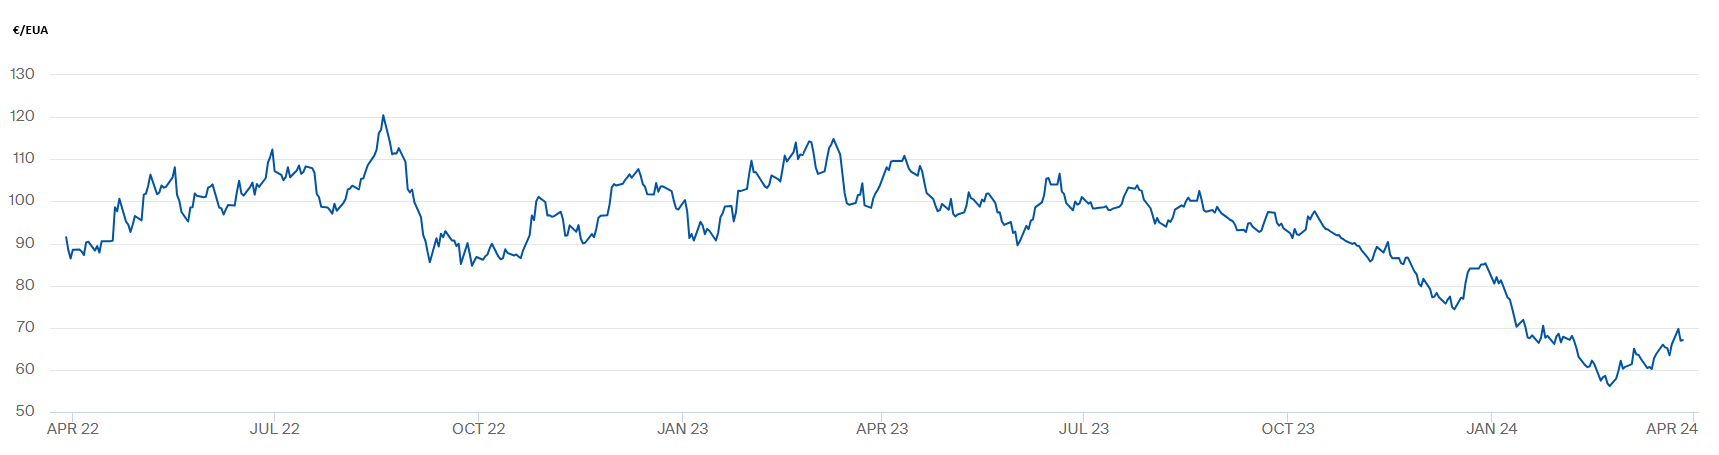
\includegraphics[width=1\linewidth]{res/tema2/precioEUA}
	\label{fig:t-emisiones}
\end{figure}
\newpage
\subsection{Influencia coste de emisión en el mercado eléctrico.}
Desde el año 2021 las centrales térmicas no tienen cantidades asignadas gratuitas y por ello, tienen que comprar derechos de emisión. Este coste repercute en el coste de la generación ofertado y, por tanto el precio de la energía como se puede ver en la figura inferior.
\begin{figure}[H]
	\centering
	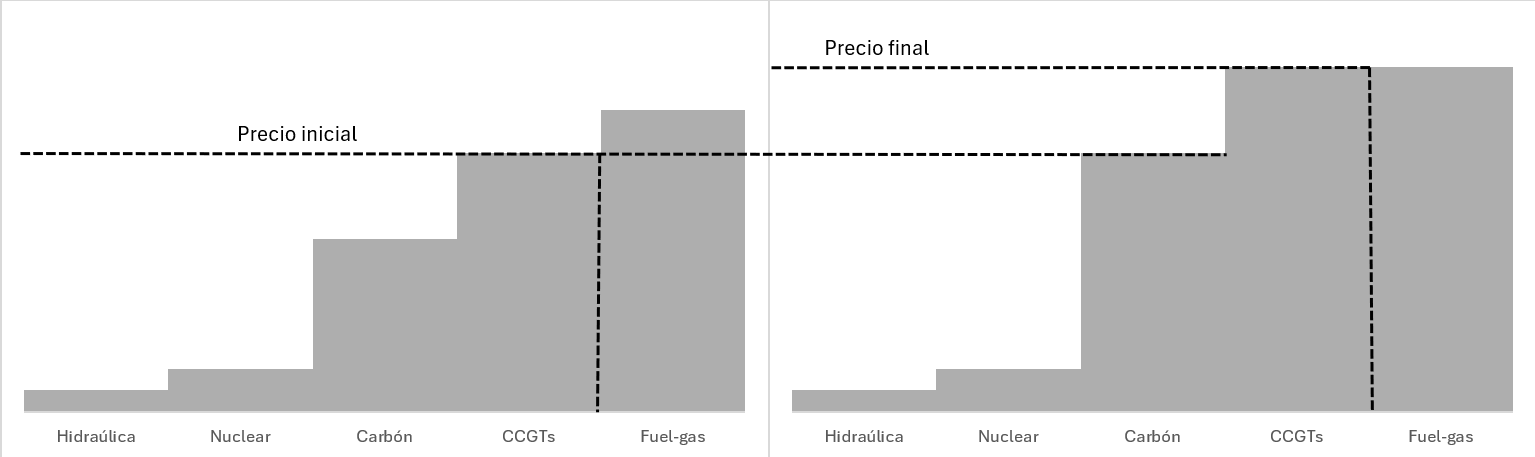
\includegraphics[width=1.2\linewidth]{res/tema2/variacionPrecio}
	\label{fig:variacionprecio}
\end{figure}
\subsection{Factor de emisión.}
El factor de emisión (fe) representa la cantidad de CO$_2$ que se genera por MWh de electricidad producida en bornes de la central:
\[fe=\frac{tCO_{2-eq}}{MWhe}=\frac{tCO_{2-eq}}{TJ}\]
Los factores de emisión se actualizan anualmente.
\subsection{Cálculo del factor de emisión.}
Para el cálculo se emplea la siguiente expresión:
\[f\left(\frac{tCO_2}{MWh}\right)=\frac{tCO_2}{TJ}\cdot\frac{3,6 TJ}{1000 MWh}\cdot\frac{100}{\eta}\]
\begin{enumerate}
	\item \textbf{Centrales térmicas de carbón:}
		El carbón es un combustible con un alto contenido en carbono y por ello genera una cantidad elevada de CO$_2$ por MWhe. El tep (tonelada equivalente petróleo) es una unidad para referir la energía con respecto a la obtenida con una tonelada de petróleo.
	\begin{table}[H]
		\centering
		\renewcommand{\arraystretch}{1.1}
		\begin{tabular}{cm{2cm}m{2cm}m{3cm}m{2cm}m{2cm}}
			\hline
			\textbf{Combustible} & \textbf{ktCO2/ktep} & \textbf{TJ/ktep} & \textbf{Factor de Emisión  combustible (tCO2/TJ)} & \textbf{Rendimiento eléctrico (\%)} & (tCO2/MWh)\\  
			\hline
			Hulla + Antracita nacional & 4,032 & 41,868 & 96,303 & 36\% & 0,96 \\
			Carbón importado           & 4,032 & 41,868 & 96,303 & 36\% & 0,96 \\
			Lignito negro              & 3,861 & 41,868 & 92,218 & 36\% & 0,92 \\
			Lignito pardo              & 3,983 & 41,868 & 95,132 & 36\% &0,95 \\ \hline
		\end{tabular}
	\end{table}
	
	\item \textbf{Centrales térmicas de ciclo combinado con gas natural:}
		Utilizan gas natural, un combustible con menor contenido en carbono que junto a su elevado rendimiento hace que tenga un menor factor de emisión.
		\begin{table}[H]
		\centering
		\renewcommand{\arraystretch}{1.1}
		\begin{tabular}{cm{2cm}m{2cm}m{3cm}m{2cm}m{2cm}}
			\hline
			\textbf{Combustible} & \textbf{ktCO2/ktep} & \textbf{TJ/ktep} & \textbf{Factor de Emisión  combustible (tCO2/TJ)} & \textbf{Rendimiento eléctrico (\%)} & (tCO2/MWh)\\  
			\hline
			Gas natural & 2,337 & 41,868 & 55,818 & 54\% & 0,37 \\
		 \hline
		\end{tabular}
	\end{table}
	\newpage
	\item \textbf{Centrales térmicas de fuel-gas:}
		Debido a su heterogeneidad se utilizan valores medios empíricos para este conjunto de centrales.
				\begin{table}[H]
			\centering
			\renewcommand{\arraystretch}{1.1}
			\begin{tabular}{cm{2cm}}
				\hline
				\textbf{Combustible}  & (tCO2/MWh)\\  
				\hline
				Gas natural & 0,77 \\
				\hline
			\end{tabular}
		\end{table}
	\item \textbf{Centrales hidráulicas, renovables y nuclear:}
		No emiten CO$_2$ para generar electricidad.
		\begin{table}[H]
			\centering
			\renewcommand{\arraystretch}{1.1}
			\begin{tabular}{cm{2cm}}
				\hline
				\textbf{Combustible}  & (tCO2/MWh)\\  
				\hline
				Centrales hidráulicas, renovables y nuclear & 0
				 \\
				\hline
			\end{tabular}
		\end{table}
	\item \textbf{Cogeneración:}
		Consiste en la producción combinada de calor y electricidad, lo que permite conseguir un rendimiento conjunto superior.
		\begin{table}[H]
			\centering
			\renewcommand{\arraystretch}{1.1}
			\begin{tabular}{cm{2cm}}
				\hline
				\textbf{Combustible}  & (tCO2/MWh)\\  
				\hline
				Cogeneración & 0,37
				\\
				\hline
			\end{tabular}
		\end{table}
	\item \textbf{Residuos:}
		Como existe una gran heterogeneidad en los combustibles empleados se toma un valor medio. En el caso de la biomasa su factor de emisión es nulo porque son neutros a nivel de emisiones. Además las emisiones de N$_2$O asociadas a los residuos no son significativas a nivel de cálculos del factor de emisión.
		\begin{table}[H]
			\centering
			\renewcommand{\arraystretch}{1.1}
			\begin{tabular}{cm{2cm}m{2cm}}
				\hline
				\textbf{Combustible} & \textbf{Rendimiento eléctrico (\%)} & (tCO2/MWh)\\  
				\hline
				Residuos &25\%& 0,24
				\\
					Biomasa &-& 0
				\\
				\hline
			\end{tabular}
		\end{table}
\end{enumerate}
\subsection{Emisiones en la combustión.}
Las fuentes de combustión que producen emisiones de CO$_2$ se calculan multiplicando el contenido de energía por un factor de emisión y oxidación (se asume igual a 1 el factor de oxidación).
\[\text{Emisiones CO}_2 = \text{Datos de la actividad} \times \text{Factor de emisión} \times \text{Factor de oxidación}\]

Los datos de actividad se expresan como el contenido de energía neto del combustible consumido [TJ] durante un periodo.
\[\text{Contenido de energía [TJ]}=\text{Combustible consumido [t o m$^3$]}\times \text{Poder calorífico combustible [TJ/t o TJ/m$^3$]}\]

El poder calorífico neto es un valor representativo de la energía liberada en la combustión en forma de calor. Esta magnitud tiene límite superior (PCS) e inferior (PCI) en función de la humedad del combustible.

\[[PCI]_s (kcal/kg)=[PCS]_s-597\cdot (9H+H_2O)\]
\begin{itemize}
	\item [-] H $\rightarrow$ \% de hidrógeno contenido en el combustible (base seca).
	\item [-] H$_2$O $\rightarrow$ \% de humedad del combustible.
\end{itemize}

\subsection{Emisiones evitadas con las energías renovables.}
Las energías renovables en España permitieron reducir la emisión de 55,6 millones de tCO$_2$ y cubrieron el 42,2\% de la demanda eléctrica.
\newpage
\section{Combustibles fósiles.}
\subsection{Combustible sólidos.}
\begin{enumerate}
	\item \textbf{Biomasa:}
		El combustible esta compuesto de materia vegetal que había sido creada a través de la fotosíntesis:
		\[6 CO_2 + 6 H_2O + 112 kcal/mol \rightarrow C_6 (H_2O)_6 + 6 O_2 ( Glucosa)\]
		Por tanto, la fotosíntesis fija al año 18.000 Mt de CO$_2$ y por tanto, quemar esta planta no produce más CO$_2$ que el que liberaría al morir por fermentación. De esta manera, se podría considerar renovable.
	\item \textbf{Carbón:}
		Es una roca de fácil combustión con aproximadamente el 50\% del peso en carbono. No obstante, en función del porcentaje de carbono cambia el poder calorífico:
		\begin{table}[H]
			\centering
			\renewcommand{\arraystretch}{1.1}
			\begin{tabular}{cccc}
				\hline
				&\textbf{Lignito} & \textbf{Hulla} & \textbf{Antracita}\\  
				\hline
			Densidad &  1,1-1,3&1,2-1,5  &1,4-1,8\\ 
			Humedad (\%) &20-50  &3-25  &3-5\\ 
			\% C & 27-31 &  37-86&89-98\\ 
			\% Volátiles &25-55  &25-50  &2-14\\ 
			PC (kcal/kg) &  2000-4000&3500-7500  &7000-8350\\ 
				\hline
			\end{tabular}
		\end{table}
		De manera general en función del tipo de carbón el combustible tiene distintas propiedades:
		\begin{enumerate}
			\item \textbf{Lignito:}
			posee un color parduzco o negro. Por lo general tiene un alto contenido en volátiles. El lignito
			negro, o carbón subbituminoso, es duro y su humedad está limitada.
			Los lignitos españoles son altamente sulfurosos. El lignito
			pardo es un carbón terroso, con alto contenido en humedad.
			\item \textbf{Hulla:}
			carbón bituminoso o carbón graso. Abarca una amplia variedad de carbones.
			Es más blando que la antracita. Arde con llama humeante y larga. Su aspecto varía desde el pardo oscuro hasta
			el negro. Son los carbones que presentan un mayor interés para la generación eléctrica.
			\item \textbf{Antracita:}
			también llamado carbón de piedra o carbón duro. De gran contenido en carbono fijo. Es duro y negro. Tiene lustre semimetálico y fractura semiconcoidal. Arde con llama azul y
			corta, sin apenas humo.
		\end{enumerate}
		El carbón esta formado por distintos elementos que condicionan su comportamiento como combustible:
		\begin{enumerate}
			\item \textbf{Carbón fijo (65-95\%):}
				A mayor porcentaje mayor poder calorífico. Permite estimar el porcentaje de generación de CO$_2$.
			\item \textbf{Hidrógeno (3-6\%):}
				Aumenta el poder calorífico y facilita la combustión.
			\item \textbf{Azufre (0,2-11\%):}
				Los carbones con alto contenido en azufre deben ser tratados porque generan SO$_2$ $\rightarrow$SO$_3$ que es altamente contaminante al provocar lluvias ácidas y ser peligroso para el ser humano.
				
				
				Los tratamientos normalmente empleados para reducir el porcentaje de azufre son:
				\begin{itemize}
					\item [-] Lavaderos de carbón: Antes de la combustión.
					\item [-] Adición de caliza: Durante la combustión (\textbf{solo lecho fluido y gasificación}).
					\item [-] Desulfuración de los gases: Después de la combustión.
				\end{itemize}
			\item \textbf{Humedad (1-60\%):}
				Provoca una disminución del poder calorífico y del rendimiento. Además necesita aire más caliente y puede provocar atascos en las tolvas.
			\item \textbf{Nitrógeno (1-1,5\%):}
				Provoca la formación de NOx en función de la temperatura de combustión.
			\item \textbf{Oxígeno (2-30\%):}
				Sirve como medida del grado de oxidación y permite reducir la cantidad de aire a aportar.
				\newpage
			\item \textbf{Materia volátil (5-40\%):}
				Se desprende durante la fase inicial del proceso de combustión, facilitan la ignición. A mayor materia volátil mayor será el humo producido.
				\begin{itemize}
					\item [-] Si tienen mucha materia volátil dan llamas cortas , calientes y muy estables. Hay pocos inquemados.
					\item [-] Si tienen poca materia volátil dan llamas largas e inestables. Se necesitan fuegos opuestos para elevar la temperatura de llama u hogares de arco que
					soporten llamas muy largas. Necesita molienda muy fina.
				\end{itemize}
			\item \textbf{Cenizas (30\%):}
				Materiales minerales no volátiles. Son residuos tras la combustión completa. Reducen la calidad del carbón.		
		\end{enumerate}
		\textbf{Combustión del carbón:} Es una reacción de oxidación con fuente de ignición donde el oxígeno se combina con el combustible para formar óxidos liberando gran cantidad de calor.
		\begin{itemize}
			\item [-] Para favorecer la combustión se pulveriza el carbón.
			\item [-] \textbf{Reacciones principales:}
			\[C+O_2\rightarrow CO_2 + 8100kcal/kg \ de \ C\]
			\[C+0,5O_2\rightarrow CO +2500kcal/kg \ de \ C\]
			\[H_2+0,5O_2\rightarrow H_2O +33600kcal/kg \ de \ H_2\]
			\[S+O_2\rightarrow SO_2 +2500kcal/kg \ de \ S\]
			\[N+O_2\rightarrow NO+O\]
			\item [-] \textbf{Condiciones necesarias combustión completa:}
			\begin{itemize}
				\item Cantidad suficiente de aire (con algo de exceso).
				\item Procurar buen grado de mezcla entre comburente y combustible (pulverización).
				\item Tiempo de residencia suficiente.
				\item Garantizar temperatura mínima en el hogar.
			\end{itemize}
			\item [-] Se considera que la combustión tiene lugar cuando la velocidad de oxidación es suficiente como para automantenerse. Cuando la velocidad de alimentación del combustible y comburente iguala a la velocidad de
			propagación de la llama entonces se estabiliza.
			\item [-]La caldera más común es la de carbón pulverizado. El diseño de estas depende del carbón a quemar.
			\begin{itemize}
				\item 240 minutos para plena carga en arranque en frío.
				\item 120 minutos para plena carga en arranque en templado (24h parada).
				\item 70 minutos para plena carga en arranque en caliente (8h parada).
				\item 60 minutos para plena carga en rearranque (2h parada).
			\end{itemize}
			\item [-] \textbf{Tipos de combustiones:} Desde el punto de vista estequiométrico puede ser completa o incompleta.
			\begin{itemize}
				\item Se considera completa cuando el combustible no quemado no supera el 2\%.
				\begin{itemize}
					\item 13 Nm$^3$ de aire por kg de carbono.
				\end{itemize}
				\item En la combustión incompleta se emite CO.
			\end{itemize}
			Se controla el tipo de combustión mediante la medida de gases a la salida de la chimenea.
			\begin{itemize}
				\item Índice emisión: 
				\[EI=\frac{\text{masa de gases emitidos}}{\text{masa de combustible quemado}}\]
				\item Masa de contaminante emitida por unidad de combustible quemado: 
				\[M/ud= \frac{EI}{Hc} (gr/MJ)\]
				\item Indice inmisión: emisión a 2m de altura sobre el suelo.
			\end{itemize}
			\item [-] \textbf{Combustión con exceso de aire:}
				Para evitar la formación de inquemados sólidos se procura una mezcla homogénea y se introduce un exceso de caudal. Para ello, se definen el exceso de aire porcentual (EA) y el coeficiente de exceso de aire (n):
				\[EA(\%)=100\times\frac{A_{exp}-A_{teorico}}{A_{teorico}}=100\times(n-1)\]
				No obstante, aumentar demasiado el exceso de aire provoca que se pierda parte del calor de la caldera.
				\begin{table}[H]
					\centering
					\renewcommand{\arraystretch}{1.1}
					\begin{tabular}{cc}
						\hline
						\textbf{Combustible}&\textbf{n}\\  
						\hline
						Gaseoso& 1,1-1,2\\
						Líquido & 1,15-1,3\\
						Pulverizado & 1,15-1,5\\ 
						\hline
					\end{tabular}
				\end{table}
				Para conocer el exceso de aire a emplear se emplea el diagrama de Oswald a partir de los contenidos de CO y CO$_2$. La región de trabajo óptima se situa en torno al 13\% de CO$_2$ en los gases de combustión.
				\begin{figure}[H]
					\begin{minipage}{0.6\linewidth}
						\centering
						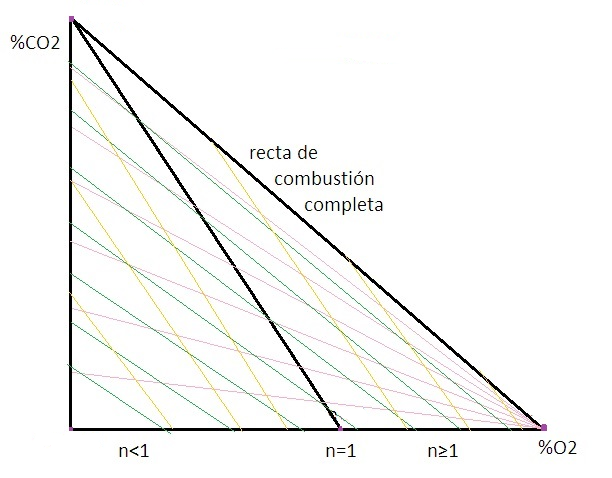
\includegraphics[width=\linewidth]{res/tema2/oswaldo}
						\label{fig:oswaldo}
					\end{minipage}%
					\begin{minipage}{0.4\linewidth}
						\centering
						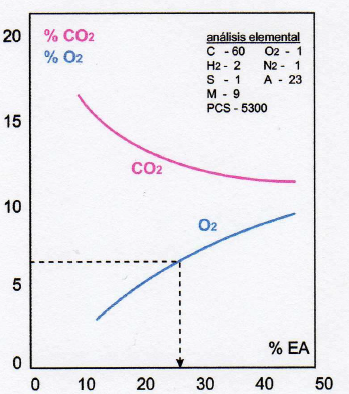
\includegraphics[width=\linewidth]{res/tema2/CO2O2}
						\label{fig:co2o2}
					\end{minipage}
				\end{figure}
				\item [-] \textbf{Balance energético en la caldera:} Se deben tener en cuenta las características energéticas y gasto del combustible frente a la calidad del vapor generado.
				
				
				Las principales pérdidas de calor en la caldera se deben a:
				\begin{itemize}
					\item Combustión incompleta: Se reduce a medida que se aumenta el exceso de aire.
					\item Calor sensible de los gases de escape: Aumenta a medida que se aumenta el exceso de aire.
					\item Sólidos inquemados: Disminuye a medida que se aumenta el exceso de aire.
				\end{itemize}
				Que resumido en un gráfico queda:
				\begin{figure}[H]
					\centering
					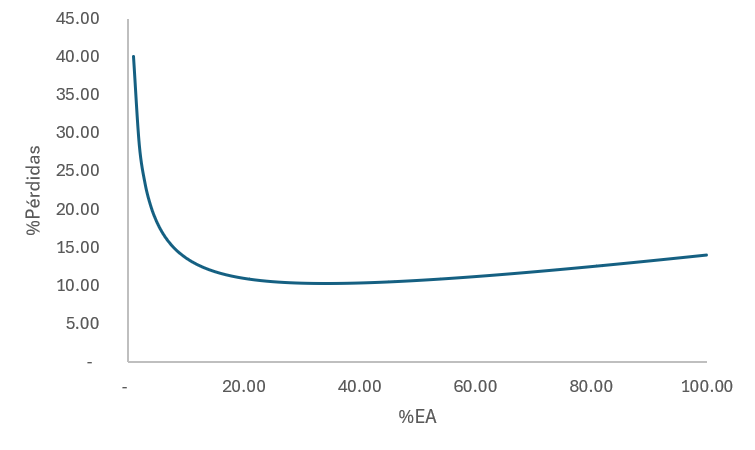
\includegraphics[width=0.5\linewidth]{res/tema2/perdidas}
					\label{fig:perdidas}
				\end{figure}
				Por tanto, el rendimiento de la caldera queda como:
				\[\eta = \frac{\text{Potencia térmica cedida al vapor sobrecalentado de salida}}{PCI \times \dot{m}_\text{combustible} \times \text{Potencia térmica aire caliente}}\approx 85-88\%\]
				En general en la caldera hay varios rendimientos:
				\begin{figure}[H]
					\centering
					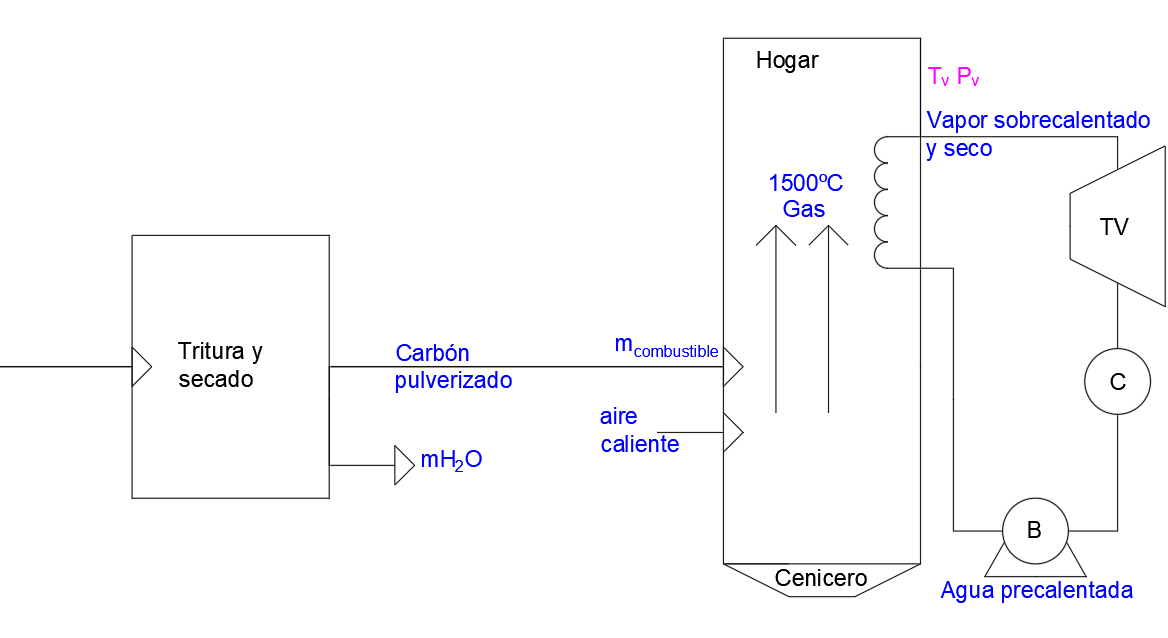
\includegraphics[width=0.7\linewidth]{res/tema2/caldera}
					\label{fig:caldera}
				\end{figure}
				Los distintos rendimientos son:
				\[\eta_{caldera}=\frac{P_{tv}}{P_{tv}+P_{aire}}\]
				\[P_{tv}=\dot{m}_{comb}\times PCI\]
				\[P_{aire}=\dot{m}_{aire}\times h_{aire}\]
				\[\eta_{planta}=\frac{P_{bc}}{P_{comb}}\]
		\end{itemize}
\end{enumerate}
\subsection{Combustible gaseosos.}
Principalmente gases naturales y materia volátil. Son de fácil combustión (poco exceso de aire). Emiten NO$_x$ y SO$_2$. Tienen peligro de explosión y por ello, requieren elevada estanqueidad.
\subsection{Combustible líquidos.}
Se compone de mezclas complejas de hidrocarburos de cadena larga. Tienen un punto de inflamación baja. Emiten NO$_x$ y SO$_2$. Provocan corrosión a baja temperatura.

\section{Impacto ambiental de las centrales térmicas de combustión.}
\subsection{Composición de gases de la combustión.}
\begin{enumerate}
	\item \textbf{Monóxido de carbono (CO):}
		Se produce por combustiones incompletas de compuestos que contienen carbono. Es un gas muy tóxico. En contacto con el oxígeno forma CO$_2$.
	\item \textbf{Materia particulada (PM):}
		Son mineral, inquemados y elementos de traza.
		\begin{itemize}
			\item [-] Una cuarta parte se recoge como ceniza mediante los ceniceros. El resto es liberado y se captura con filtros ciclónicos o electrostáticos.
			\item [-] Los elementos de traza (Hg y Se) se capturan mediante filtros de resinas.
		\end{itemize}
		Los minerales que se consideran contaminantes son:  Be, Cr, Mn, Co, Ni, As, Se, Cd, Sb, Hg y Pb.
	\item \textbf{Compuestos orgánicos:}
		Se pueden encontrar como gas si son volátiles (metano y benceno) o en la superficie de partículas como hidrocarburos aromáticos policlínicos.
	\item \textbf{Óxidos de azufre (SO$_2$, SO$_3$, SH$_2$):}
		Provocan lluvia ácida. En las calderas se forma SO$_2$ que posteriormente forma el resto de óxidos.
		\begin{figure}[H]
			\centering
			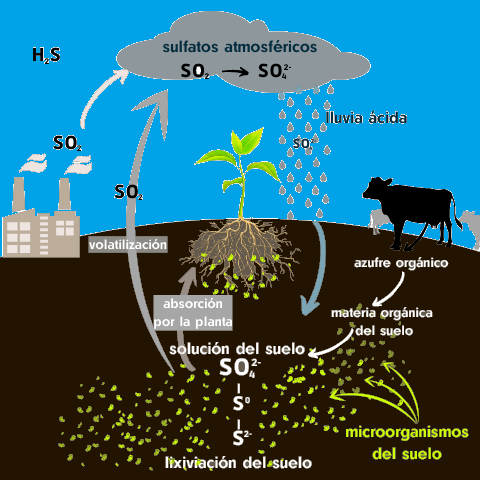
\includegraphics[width=0.4\linewidth]{res/tema2/sicloazufgre}
			\label{fig:sicloazufgre}
		\end{figure}
		
	\item \textbf{Óxidos de nitrógeno (NO$_x$):}
		Provocan lluvia ácida, destrucción de la capa de ozono y smog fotoquímico:
		\begin{itemize}
			\item [-] \textbf{NO$_2$:} precursor del efecto invernadero. Son muy absorbentes de radiación infrarroja. Se genera a partir del NO con exceso de oxígeno.
			\item [-] \textbf{NO:} reducción del ozono en la estratosfera (es menos tóxico que el NO$_2$). Se genera por la alta temperatura de la caldera con el N$_2$ del aire. 
			\item [-] \textbf{N$_2$O:} reducción del ozono en la troposfera. Se produce en mezclas pobres con poco O$_2$.
		\end{itemize}
\end{enumerate}
\subsection{Tratamientos para reducción de emisiones.}
\begin{enumerate}
	\item \textbf{Óxidos de azufre (SO$_2$):}
	Se clasifican en función del momento de la combustión en el que se realice el tratamiento:
	\begin{enumerate}
		\item \textbf{Precombustión:} 
		\begin{itemize}
			\item [-] Uso de carbones de alta calidad.
			\item [-] Combustión mixta con gas natural.
			\item [-] Lavado y desulfuración del combustible.
			\item [-] Gasificación del carbón.
		\end{itemize}
		\item \textbf{Durante la combustión:}
		\textbf{Solo en calderas de lecho fluidificado} se puede introducir caliza CaCO$_3$ para fijar el azufre. 
		\item \textbf{Postcombustión:}
			Se manipulan los gases mediante torres de lavado por vía húmeda o semihumeda con un rendimiento del 40\%.
			
			El proceso de absorción química en las torres de lavado es el siguiente:
			\[SO_2+H_2O\rightarrow H_2SO_4\]
			\[CaCO_3+H_2SO_4\rightarrow CaSO_3+CO_2+H_2O\]
			\[CaSO_3+0,5O_2+H_2O\rightarrow CaSO_4+2H_2O\]
			\begin{figure}[H]
				\centering
				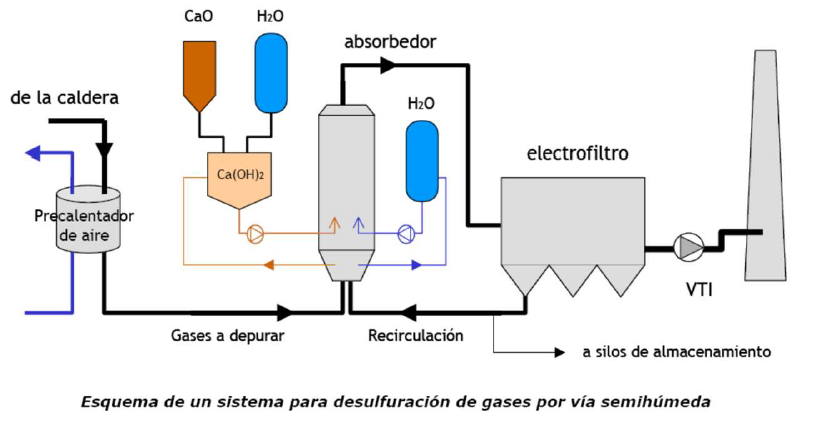
\includegraphics[width=0.5\linewidth]{res/tema2/desulfuric}
				\label{fig:desulfuric}
			\end{figure}
			
	\end{enumerate}
	\item \textbf{Óxidos de nitrógeno (NO$_x$):}
	\begin{itemize}
		\item [-] \textbf{Técnicas primarias:} Se basan en el control del proceso de combustión. Modificacando los siguientes parámetros que reducen las emisiones de NO$_x$ a costa del rendimiento:
		\begin{itemize}
			\item Reducción de la temperatura.
			\item Disminución del exceso de aire.
			\item Inyección de vapor.
			\item Combustión con O$_2$ puro.
			\item Combustible con menos N$_2$.
			\item Uso de catalizadores.
		\end{itemize}
		El problema de los NO$_x$ disminuye en las calderas de lecho fluido debido a que trabajan a 900° C en lugar de los 1500° C de una caldera convencional.
		\item [-] \textbf{Técnicas secundarias:} Se basan en reducir las emisiones de gases tras la combustión:
		\begin{itemize}
			\item Absorción química con $H_2SO_4$:
			
\begin{figure}[H]
	\centering
	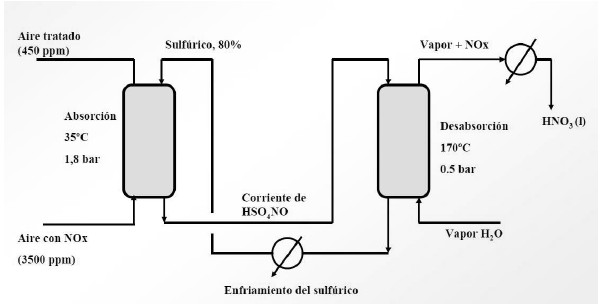
\includegraphics[width=0.5\linewidth]{res/tema2/H2so4abs}
	\label{fig:h2so4abs}
\end{figure}
	\item Proceso TYCO: incorpora eliminación $SO_2$ y recupera ácidos:
	
\begin{figure}[H]
	\centering
	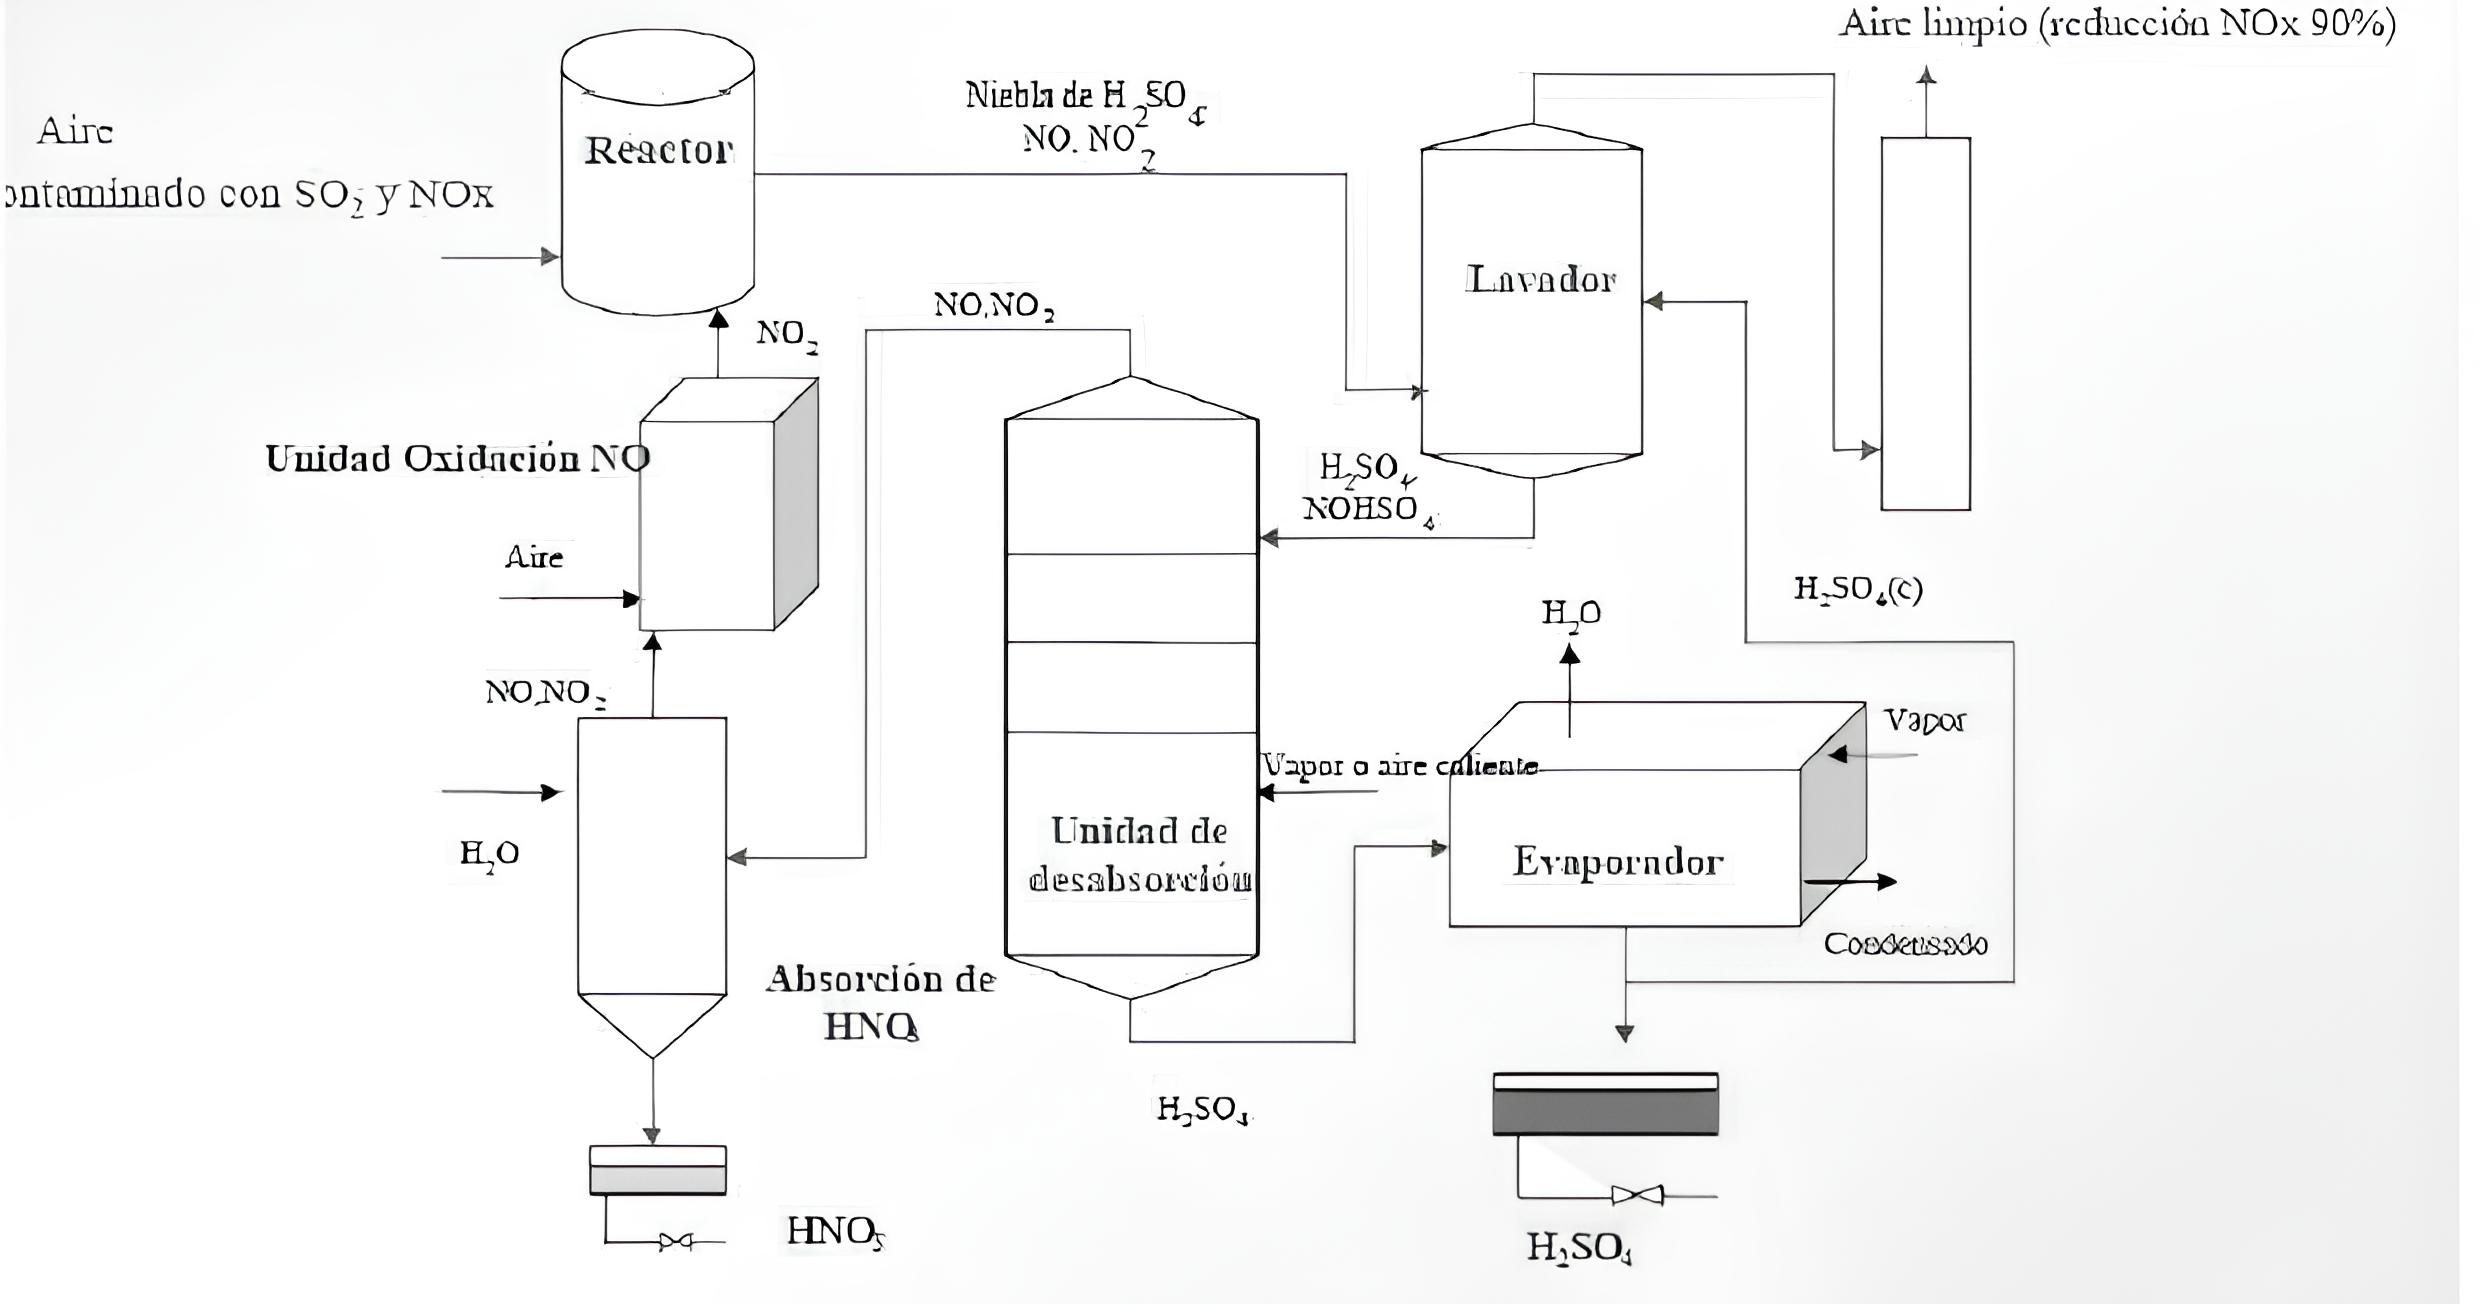
\includegraphics[width=0.5\linewidth]{res/tema2/tyci+}
	\label{fig:tyci}
\end{figure}
\item Reducción catalítica selectiva: se emplea amoniaco que al reaccionar con los NO$_x$. Tiene una eficiencia de eliminación del 85\%.
\[6NO_x+4xNH_3\rightarrow [2x+3]N_2+6xH_2O\]
		\end{itemize}
	\end{itemize}
	\item \textbf{Materia particulada (PM):} Se trata mediante filtros ciclónicos y electrostáticos tras la combustión. Tienen un gran consumo energético 12\% del autoconsumo.
\end{enumerate}
\begin{figure}[H]
	\centering
	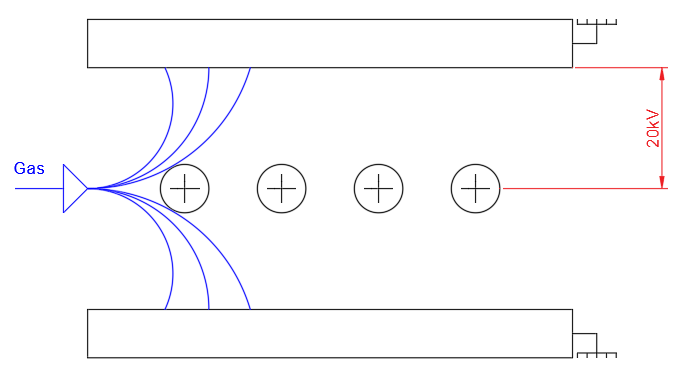
\includegraphics[width=0.7\linewidth]{res/tema2/filtroelectrostatico}
	\label{fig:filtroelectrostatico}
\end{figure}

\subsection{Impacto ambiental centrales térmicas.}
Anteriormente se han discutido principalmente las centrales térmicas de carbón, pero si el combustible es líquido o sólido cambia ligeramente el impacto ambiental.
\begin{itemize}
	\item \textbf{Combustible líquido:}
		El impacto ambiental es menor que el de las de carbón aunque el uso de estas centrales esta disminuyendo. Emite menos gases contaminantes y la materia particulada esta compuesta principalmente por hollín. 
		
		
		Los combustibles principales usados son los gasóleos (comparten mercado con la automoción) y los fuelóleos (uso exclusivo en instalaciones térmicas).
		
		El principal inconveniente de los fuelóleos es su alto contenido en azufre.
	\item \textbf{Gas natural:}
		El gas natural es un combustible con muy alto poder calorífico y son las centrales de combustión de combustibles fósiles con menor impacto ambiental aunque tienen problemas de emisiones de NO$_x$ y generan elevada contaminación acústica.
		
		Cabe destacar, que otra ventaja es que como se recibe continuamente gas no es necesario invertir en sistemas de almacenamiento y, además, no necesita tratamiento previo. Que también como durante el transporte se entierran la contaminación producida por fugas es despreciable.
\end{itemize}
\section{Impacto ambiental centrales nucleares.}
Tienen el mismo impacto térmico y químico que las centrales térmicas convencionales aunque no libera gases contaminantes. No obstante, presenta el problema de los residuos radioactivos.
\subsection{Tipos de radioactividad.}
La radioactividad es un efecto producido por descomposición espontánea de un núcleo inestable en otro más estable. Los tipos de radiación principales son:
\begin{itemize}
	\item [-] La radiación alfa ($\alpha$) está formada por núcleos de helio. No es capaz de atravesar el papel.
	\item [-] La radiación beta ($\beta$) está constituida por electrones. No es capaz de atravesar el acero.
	\item [-] La radiación gamma ($\gamma$) es de naturaleza electromagnética. No es capaz de atravesar el plomo.
	\item [-] Radiación neutrónica (n). No es capaz de atravesar el cemento.
\end{itemize}
\subsection{Medida de la radioactividad.}
Se mide mediante la cantidad de radiación emitida. 
\begin{itemize}
	\item [-] Si la radiación afecta al ser humano se mide en Sievert (Sv): Unidad de dosis equivalente.
	\item [-] Si la radiación afecta a un objeto se mide en Gray (Gy): Unidad de dosis absorbida. Se define como la dosis de radiación que transfiere una energía de 1 julio a 1 kilogramo masa de
	material irradiado
	\item [-] Si se habla de fuente emisora de radiación (material radiactivo) se emplea el Becquerel (Bq). Se define como la actividad de un material que experimenta una desintegración por segundo.
	
\begin{figure}[H]
	\begin{center}
	\scalebox{0.8}[0.8]{
		\begin{tikzpicture}
			\def\printonlylargeenough#1#2{\unless\ifdim#2pt<#1pt\relax
				#2\printnumbertrue
				\else
				\printnumberfalse
				\fi}
			\newif\ifprintnumber
			\pie[rotate=90, text=legend, before number=\printonlylargeenough{1}, after number=\ifprintnumber\%\fi]{
				36.7/Inhalación de radón,
				29.1/Aplicaciones médicas,
				13.1/Radiación suelo,
				10.2/Radiación cosmica,
				9.9/Propio Cuerpo,
				0.6/Exposición profesional: 0.6\%,
				0.3/Poso radioactivo 0.3\%,
				0.1/Centrales nucleares 0.1\%
			}
		\end{tikzpicture}
}	\end{center}
\end{figure}	
\end{itemize}
\subsection{Clasificación de los residuos radioactivos.}
\begin{itemize}
	\item [-] \textbf{Según el estado de agregación.}
	\begin{enumerate}
		\item \textbf{Residuos gaseosos:} Se debe distinguir entre isotopos radioactivos y el aire. Mediante filtros de alta eficiencia (HEPA) se retiene el 99,9\% de las partículas de 0,3 $\mu$m.
		\item \textbf{Residuos líquidos:} Principalmente tritio. Se eliminan con operaciones de filtración, centrifugación, precipitación química,
		intercambio iónico y evaporación .
		\item \textbf{Residuos sólidos:} Se clasifican en alta, media o baja actividad.
	\end{enumerate}
	\item [-] \textbf{Según la radiactividad.}
	\begin{enumerate}
		\item \textbf{Sólidos de actividad media y baja:} Tienen una vida media de menos de 30 años. Se mezclan con aglomerantes y se almacenan en depósitos. 
		
		España genera 1220 m$^3$ al año. Los residuos dejan de ser peligrosos a los cientos de años con lo cual es seguro almacenarlos en instalaciones permanentes en superficie. 
		\item \textbf{Sólidos de alta actividad:} Están constituidos por el combustible gastado. Contienen radionucleidos de larga vida media que tardan miles de años en llegar a niveles seguros de radiación. 
		
		Se enfrían en piscinas en la propia central durante 5 años y después se embuten en vidrio para ser almacenados en lugares de almacenamiento centralizado. Actualmente en España estos residuos se almacenan en el extranjero con un coste de 49.545,17€/día (en teoria deberian haber vuelto a España en 2010).
	\end{enumerate}
	La generación media de una central tipo de 1.000 MW es de 20 toneladas de uranio al
	año (combustible gastado), de 50 m$_3$ (centrales con tecnología PWR) y 130 m$^3$
	(centrales BWR) de residuos de media y baja actividad.
	
	Anteriormente el precio de la gestión de los residuos radiactivos recaía sobre el consumidor de la energía eléctrica. No obstante, actualmente se plantea que las nucleares paguen esta gestión.
\end{itemize}
\subsection{Gestión del combustible gastado.}
Cuando se descarga el combustible del reactor todavía hay gran cantidad de energía puede ser utilizada al solo haberse gastado el 5\% de la energía inicial.
\begin{itemize}
	\item [-] Si se almacena tras su uso en instalaciones de almacenamiento geológico profundo se habla de ciclo abierto.
	\item [-] Si se reprocesa el combustible gastado para ser reutilizado se habla de ciclo cerrado. En el ciclo cerrado se recupera el combustible fabricando pastillas de óxido de uranio (UO$_2$) y óxido de plutonio (PuO$_2$) que se denominan combustible MOX.
\end{itemize}
Las piscinas donde se almacena el combustible gastado suelen ser de agua por su alto coeficiente de transmisión del calor y sus propiedades como blindaje. Hoy en día presentan una problemática debido a que las piscinas de las centrales nucleares españolas están saturadas.
\section{Impacto ambiental centrales hidroeléctricas.}
De acuerdo con la IHA (International Hydropower Association), existen varios aspectos clave que hay que tener en
cuenta para mantener el potencial hidroeléctrico con un desarrollo sostenible en materia medioambiental:
\begin{enumerate}
	\item \textbf{Calidad del agua:} Puede reducir la cantidad de oxígeno en agua, su temperatura y la estratificación de los sedimentos.
	\item \textbf{Erosión y transporte de sedimentos:} Cambia la cantidad de sedimentos transportados y a largo plazo puede cambiar la forma del río por el cambio de la erosión.
	\item \textbf{Hidrología y flujos mediambientales del río:} Como cambia la hidrología y el entorno del río afecta a la fauna y a actividades humanas que se desarrollaban en el río.
	\item \textbf{Especies en peligro de extinción:}  La construcción de una presa puede poner en serio riesgo a especies amenazadas o únicas, debido a los
	cambios del hábitat natural.
	\item \textbf{Paso de especies:} Muchas especies recorren el río a lo largo de su ciclo de vida en uno o ambos sentidos. En muchos lugares,
	la migración de peces (como el salmón) es un acontecimiento anual, que se ve seriamente dificultado por las
	presas.
	\item \textbf{Plagas animales y vegetales en los embalses:} Los cambios en las condiciones del agua pueden facilitar la colonización de especies
	ajenas al entorno, creando plagas.
	\item \textbf{Aspectos sanitarios:} Los cambios producidos en el entorno por la construcción de presas pueden afectar a la salud pública,
	influyendo en la transmisión de enfermedades.
	\item \textbf{Actividades de construcción:} Las actividades de construcción provocan alteraciones en el medio acuático y terrestre.
\end{enumerate}
\section{Impacto ambiental transporte y transformación energía eléctrica.}
Tienen un impacto menor que las instalaciones de producción.
\begin{enumerate}
	\item \textbf{Líneas de transporte y distribución:} Se utilizan terrenos para la instalación de torres que provocan impacto visual y afectan a la avifauna.
	\item \textbf{Subestaciones de transformación:}
	Provocan una pérdida de suelo y vegetación, emiten ruidos y pueden provocar contaminación de agua por fugas.
	\item \textbf{Redes de baja tensión y centros de transformación:} Producen impacto visual y emisión de ruidos.
	\item \textbf{Campos electromagnéticos:} Los campos eléctricos son proporcionales a la tensión y los campos magnéticos a la intensidad.	
\end{enumerate}
		\section{Tema 3: Conservación de la masa}
\subsection{Teorema del transporte de Reynolds}
\begin{figure}[H]
	\centering
	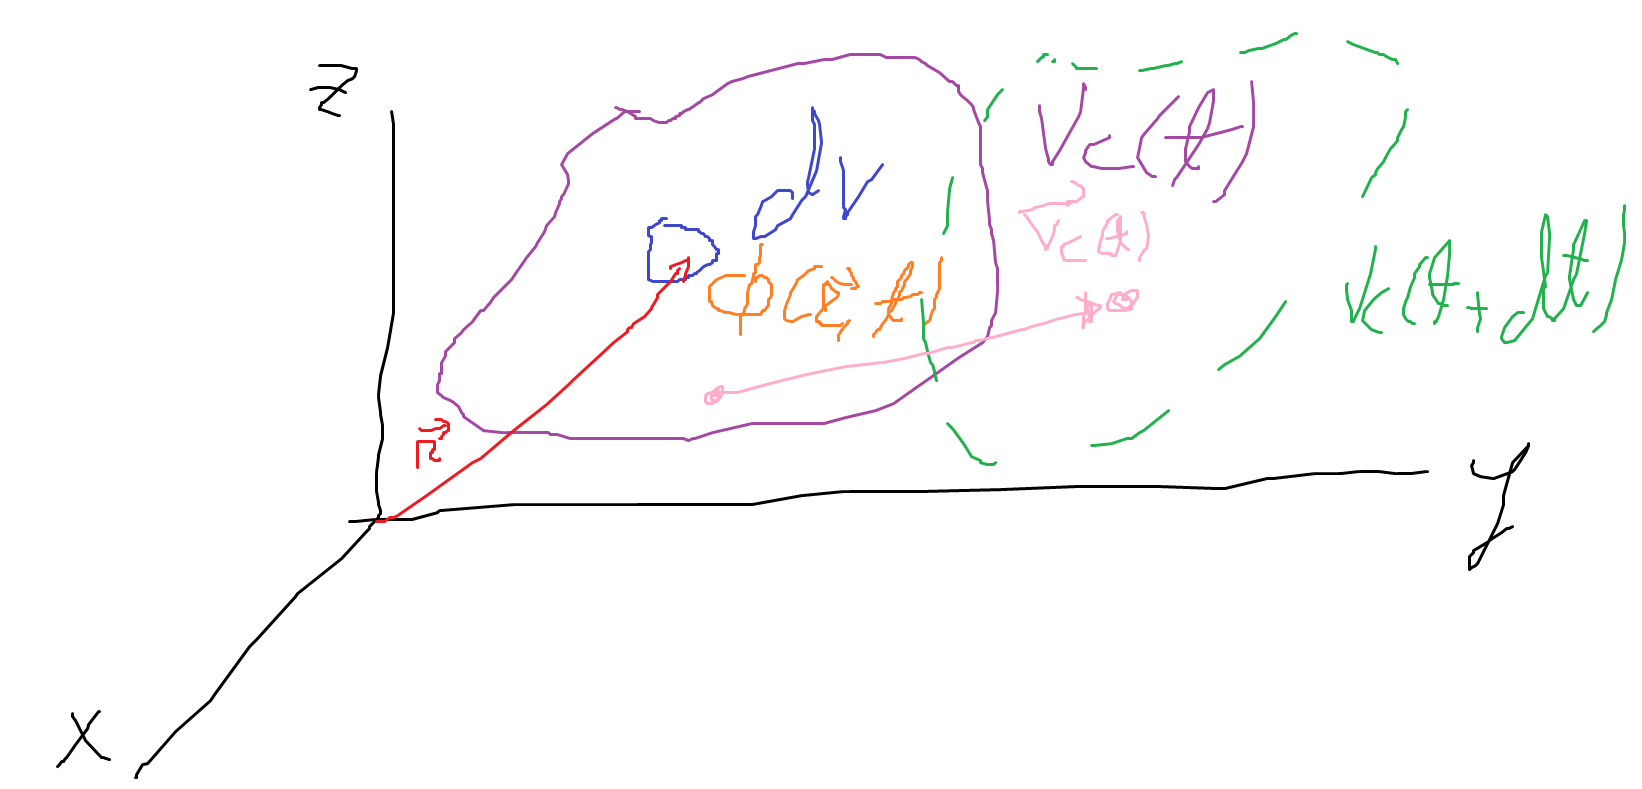
\includegraphics[width=0.7\linewidth]{imagenesTema3/magnitudesReynolds}
	\caption{}
	\label{fig:magnitudesreynolds}
\end{figure}

\[\Phi=\text{Función que depende del espacio y tiempo en general}\rightarrow\Phi=f(\vec{r},t)\]

Nos interesa conocer:
\[\frac{d}{dt}\int_{V_c(t)} \Phi(\vec{r},t) \,dV=\lim_{\Delta t \to 0} \left[\int_{V_c(t+dt)} \Phi(\vec{r},t+dt) \,dV-\int_{V_c(t)} \Phi(\vec{r},t) \,dV\right]\]
Se hace el desarrollo de Taylor en t del primer término:
\[\frac{d}{dt}\int_{V_c(t)} \Phi(\vec{r},t) \,dV=\int_{V_c(t)} \frac{\partial}{\partial t}\Phi(\vec{r},t) \,dV+\lim_{\Delta t \to 0} \frac{1}{\Delta t}\left[\int_{V_c(t+dt)} \Phi(\vec{r},t) \,dV-\int_{V_c(t)} \Phi(\vec{r},t) \,dV\right]\]

Hay que estudiar la velocidad del volumen de control de tal manera que, solo afecta la velocidad paralela a la normal porque es lo que provoca expansión o compresión del mismo, la velocidad tangencial lo "gira":
\[dV=\vec{v}_c\cdot\vec{n}dS\Delta t\]
Por tanto:
\[\frac{d}{dt}\int_{V_c(t)} \Phi(\vec{r},t) \,dV=\int_{V_c(t)} \frac{\partial}{\partial t}\Phi(\vec{r},t) \,dV+\oint_{S_c(t)} \Phi(\vec{r},t)\vec{v}_c\cdot\vec{n}\Delta t \,dS\]

Si queremos podemos imponer que (hablando en tema de volumen fluido):
\[V_c(t)=V_{fluido}(t)=V_f(t)\]
\[\frac{d}{dt}\int_{V_f(t)} \Phi(\vec{r},t) \,dV=\int_{V_f(t)} \frac{\partial}{\partial t}\Phi(\vec{r},t) \,dV+\oint_{S_f(t)} \Phi(\vec{r},t)\vec{v}\cdot\vec{n}\Delta t \,dS\]

Si tomamos un tiempo t* paramétrico tal que $V_c(t*)=V_F(t*) \rightarrow \int_{V_c(t*)}\frac{\partial \Phi}{\partial t}\,dV\approx \int_{V_f(t*)}\frac{\partial \Phi}{\partial t}\,dV$ Solo en ese instante t*

Si se restan las ecuaciones de Volumen de control y la de los movimientos fluidos queda (Teorema de Reynolds del transporte (problemas)):

\[\frac{d}{dt}\int_{V_f(t)}\Phi(\vec{r},t)\,dV=\frac{d}{dt}\int_{V_c(t)}\Phi(\vec{r},t)\,dV+\oint_{S_c(t)} \Phi(\vec{r},t)\left[(\vec{v}-\vec{v}_c)\cdot\vec{n}\right]\Delta t \,dS\]

(TH Reynolds para teoria)
\[\frac{d}{dt}\int_{V_f(t)} \Phi(\vec{r},t) \,dV=\int_{V_f(t)} \frac{\partial}{\partial t}\Phi(\vec{r},t) \,dV+\oint_{S_f(t)} \Phi(\vec{r},t)\vec{v}\cdot\vec{n}\Delta t \,dS\]

Término de variación local:
\[\int_{V_f(t)} \frac{\partial}{\partial t}\Phi(\vec{r},t) \,dV\]
Térimno de variación convectiva:
\[\oint_{S_f(t)} \Phi(\vec{r},t)\vec{v}\cdot\vec{n}\Delta t \,dS\]


Si la magnitud $\Phi = \rho$ Se obtiene la ecuación de conservación de la masa en forma integral:
Es igual a 0 porque no se pierde masa:
(Problemas)
\[\frac{d}{dt}\int_{V_f(t)}\rho\,dV=\frac{d}{dt}\int_{V_c(t)}\rho\,dV+\oint_{S_c(t)} \rho\left[(\vec{v}-\vec{v}_c)\cdot\vec{n}\right]\Delta t \,dS=0\]
(Teoría)
\[\frac{d}{dt}\int_{V_f(t)} \rho \,dV=\int_{V_f(t)} \frac{\partial \rho}{\partial t} \,dV+\oint_{S_f(t)} \rho\vec{v}\cdot\vec{n}\Delta t \,dS=0\]

Si $V_f(t)\approx dV_f(t)$ entonces y aplicando el teorema de gauss se llega a la ecuación diferencial de la masa o forma conservativa:
($\oint_S \varphi \cdot \vec{n}\,dS=\int_V \vec{\nabla}\cdot\varphi\,dV$)
\[\lim_{dV \to 0}\left[\frac{\partial \rho}{\partial t} dV+\vec{\nabla}\cdot\left(\rho\vec{v}\right)dV\right]=0\]
\[\frac{\partial \rho}{\partial t} +\vec{\nabla}\cdot\left(\rho\vec{v}\right)=0\]
Término local de masa: 
\[\frac{\partial \rho}{\partial t}\]
Término convectivo de masa:
\[\vec{\nabla}\cdot\left(\rho\vec{v}\right)\]

		\chapter{Cobertura de la demanda. Mercado eléctrico.}
\section{Explotación del mercado eléctrico.}
La energía eléctrica se genera en grandes concentradas de forma concentrada y posteriormente se transmite a grandes distancias donde el equilibrio se obtiene de las curvas de oferta y demanda.


Una misión importante de la red es la de ajustar la energía generada a la demandada con unos valores de tensión (Control Q-U) y frecuencia (Control P-f).
\section{Curva de demanda diaria.}
La demanda varia constantemente tanto hora a hora como diariamente. Esta demanda se refleja en las curvas de carga o demanda donde la diferencia entre ambas equivale a las pérdidas en la red ($\approx$12\%).

\begin{itemize}
	\item [-]\textbf{Energía producida:} se entiende en barras de la central, descontando el autoconsumo.
	\item [-]\textbf{Energías consumida:} se obtiene de la suma del consumo de los abonados.
\end{itemize}
\begin{figure}[H]
	\begin{minipage}{0.5\linewidth}
		\centering
		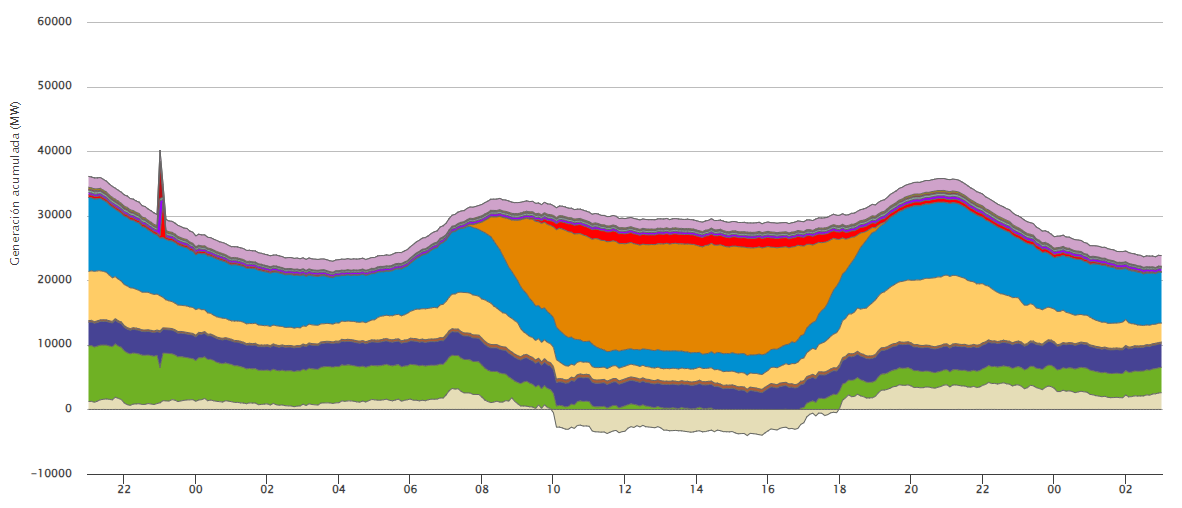
\includegraphics[width=0.7\linewidth]{res/tema4/demandaDia}
		\label{fig:demandadia}
	\end{minipage}
	\begin{minipage}{0.5\linewidth}
		\centering
		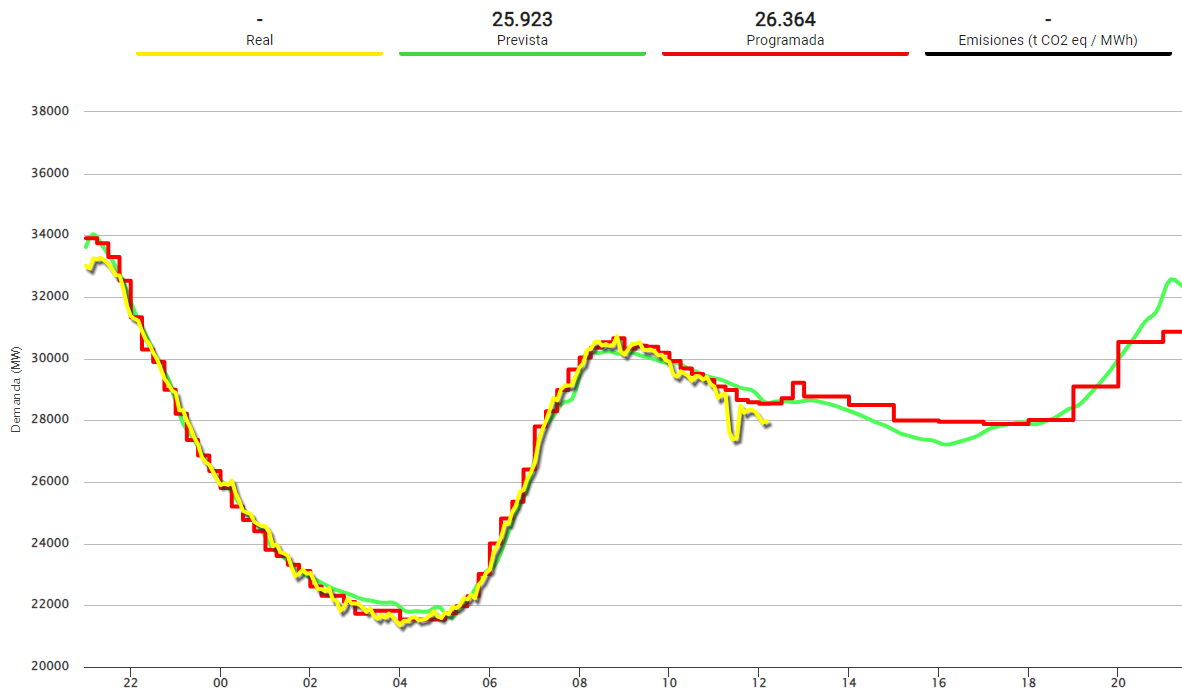
\includegraphics[width=0.7\linewidth]{res/tema4/demandaDia1}
		\label{fig:demandadia1}
	\end{minipage}
\end{figure}
La curva de carga o de demanda se predice mediante la estadística acumulada de muchos años ya que para fijar el precio es necesaria esta previsión (tiene un error asociado del 2\%). En estos datos, se pueden apreciar típicamente tres picos de consumo (12, 16 y 20 horas) que llevan a la tarifa PVPC (Precio de venta al pequeño consumidor) con discriminación horaria en horas valle, llano y punta.


Cabe destacar, como los factores locales tienen mucho peso sobre la demanda real como la temperatura, grandes eventos, ...

\section{Pérdidas en la red.}
Son un coste de operación necesario para mover la energía desde donde se produce (Galicia y Cataluña como pozos) hacia donde se consume (Madrid y Barcelona como sumideros). 
\begin{itemize}
	\item [-] Red de transporte 1-2\%
	\item [-] Red de distribución 4-6\%
	\item [-] Red baja tensión 7-10\%
\end{itemize}
\section{Gestión de la red.}
La empresa encargada de la gestión de la red es Red Eléctrica Española (REE) que recibe a través de su red de fibra óptica las potencias activa y reactiva en varios puntos de la red. La gestión se realiza desde el Centro de Control Eléctrico (CECOEL).

Para realizar esta gestión REE debe tener en cuenta muchas incertidumbres asociadas a defectos en generadores y la red lo cual provoca un sobredimensionamiento del sistema.
\subsection{Incidencias no previstas.}
Cuando ocurren incidencias graves, normalmente asociadas a una falta en la generación REE debe aplicar cortes a las industrias acogidas a contratos de interrumpibilidad.
\subsection{Configuración sistema eléctrico de potencia.}
El sistema léctrico de potencia se compone de lo siguientes elementos:
\begin{itemize}
	\item [-] \textbf{Generación:} Se genera en barras del generador de 6-30 kV a 50Hz con potencias de hasta 1500 MVA.
	\item [-] \textbf{Redes de Transporte:} Esta formada por un elevado número de nodos con topología mallada a los que se conectan los generadores y consumidores a una tensión de 220-400kV.
	\item [-] \textbf{Redes de Distribución:}  Las longitudes de estas líneas no superan los 25 km y normalmente son aéreas. En núcleos urbanos suelen ser malladas y en zona rural radiales. Se distribuye de 132-15kV.
	\item [-] \textbf{Centros de transformación:} Se reduce la tensión de media a baja tensión.
	\item [-] \textbf{Consumidores:} Red de distribución a 230/400V.
\end{itemize}
\section{Funcionamiento del mercado eléctrico.}
Desde la Ley 54/1997 se liberalizó el sector eléctrico para permitir la libre competencia con las siguientes características:
\begin{itemize}
	\item [-] Libertad de construcción de nuevas centrales de producción de electricidad.
	\item [-] Competencia entre las empresas productoras de electricidad en un mercado de ofertas.
	\item [-] Libertad progresiva de los consumidores para elegir el suministrador que deseen y acordar con
	él las condiciones y precio del kWh.
	\item [-] Libertad de comercialización de la electricidad.
	\item [-] Libertad de comprar o vender electricidad a empresas y consumidores de otros miembros de
	la UE.
	\item [-] Separación jurídica de actividades:
	\begin{itemize}
		\item \textbf{Reguladas:} transporte, distribución y gestión del sistema.
		\item \textbf{No reguladas:} generación y comercialización
	\end{itemize}
	\item [-] Sostenibilidad económica y financiera:
	\begin{itemize}
		\item Garantizar el suministro al mínimo coste.
		\item Retribución de actividades con base en criterios objetivos, transparente y homogéneos.
		\item Marco normativo que garantice la estabilidad financiera.
		\item  Actualización de los peajes de acceso a través de cargos.
	\end{itemize}
\end{itemize}
La explotación del mercado eléctrico se realiza conjuntamente entre:
\begin{itemize}
	\item 
	\item
	\item
\end{itemize}
\subsection{Actividades principales.}
g
\subsection{Reparto de la distribución de energía eléctrica.}
g
\subsection{Comercialización.}
g
\subsection{Organización.}
g
\subsection{Instituciones reguladoras.}
g
\subsection{Operador del mercado (OMIE).}
g
\subsection{Operador del sistema (REE).}
g
\section{Mercado ibérico (MIBEL).}
g
\section{Interconexiones con el extranjero.}
g
\subsection{Francia.}
g
\subsection{Portugal.}
g
\subsection{Marruecos.}
g
\subsection{Gestión de las interconexiones.}
g
\section{Mercado intradiario.}
g
\subsection{Secuencia de los procesos del mercado.}
g
\subsection{Mercados a plazo.}
g
\subsection{Mercado organizado diario (casación horaria).}
g
\subsection{Tipos de oferta de venta de energía.}
g
\subsection{Proceso de casación.}
g
\subsection{Curva de oferta de venta de energía.}
g
\subsection{Influencia fuentes renovables.}
g
\subsection{Retribuciones para amortizar costes fijos.}
g
\subsection{Curva de demanda.}
g
\section{Mercado de restricciones técnicas.}
g
\section{Mercado de servicios complementarios.}
g
\subsection{Regulación primaria.}
g
\subsection{Regulación secundaria.}
g
\subsection{Control de tensión.}
g
\subsection{Reservas de potencia.}
g
\subsection{Gestión de desvíos.}
g
\subsection{Regulación terciaria.}
g
\section{Precio medio final.}
g
\subsection{Costes recogidos en la tarifa eléctrica (PVPC).}
g
\section{Programación de la generación de electricidad.}
g
\subsection{Curva acumulada de demanda anual.}
g
\subsection{Curva de demanda anual.}
g
\subsection{Parámetros principales curva de demanda.}
g
\subsection{Curva acumulada de generación anual.}
g
\subsection{Parámetros principales curva de generación.}
g
\section{Reserva de potencia.}
g
\subsection{Características estáticas.}
g
\subsection{Características dinámicas.}
g
\subsection{Secuenciamiento óptimo de grupos.}
g
\section{Costes de generación.}
g
\subsection{Comparativa de costes.}
g
\subsection{Coste de inversión o fijo.}
g
\subsection{Costes variables.}
g
\subsection{Coste total.}
g
\section{Aspectos técnicos de la producción de energía.}
g
		\chapter{Selectividad interruptores automáticos de baja tensión}
En caso de defecto debe abrir el interruptor automático situado inmediatamente aguas arriba del defecto y sólo él.
\begin{figure}[H]
	\centering
	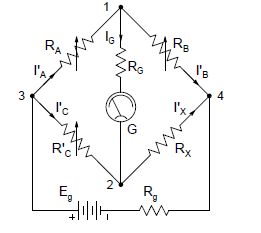
\includegraphics[width=0.4\linewidth]{Images/18}
\end{figure}
\section{Selectividad Total}
Para cualquier valor de la intensidad de defecto “aguas abajo” de B, el interruptor automático B es el único en desconectar 
\section{Selectividad Parcial}
Para ciertos valores de la intensidad de defecto “aguas abajo” de B, el interruptor B es el único en desconectar, pero para otros abren los dos interruptores, A y B
\section{Selectividad frente a sobrecargas}
\section{Selectividad frente a cortocircuitos}
\section{Selectividad frente a cortocircuitos moderados}
\section{Coordinación entre interruptores automáticos}
\section{Selectividad lógica}
		\chapter{Generador síncrono.}

	\section{Generalidades.}
		Los generadores síncronos o alternadores trifásicos autoexcitados en corriente continua que se usan en las centrales eléctricas se diferencian en función del número de vueltas de sus máquinas motrices.
		
		
		Velocidad síncrona en régimen permanente:
		
		\[n = \dfrac{60\cdot f}{p}\,[rpm]\]
		
		Donde $f$ es la frecuencia industrial y $p$ el número de pares de polos.
		
		
		\subsection{Aplicaciones de la máquina síncrona.}
			\begin{itemize}
				\item \textbf{Como generador:}
					\begin{itemize}
						\item Suministro de potencia a la red.
						\item Suministro de emergencia (hospitales, centros comerciales...).
						\item Instalaciones aisladas (redes rurales).
					\end{itemize}
					
				\item \textbf{Como motor:}
					\begin{itemize}
						\item Aplicaciones con velocidad constante (bombeo en centrales hidráulicas reversibles).
						\item Compensador síncrono en centrales (regulación del factor de potencia).
					\end{itemize}
			\end{itemize}
			
		\subsection{Aspectos constructivos.}
			\begin{itemize}
				\item \textbf{Inducido:}
					\begin{itemize}
						\item Se alimenta con corriente alterna trifásica.
						\item Con expansiones polares y devanado concentrado.
						\item Cilíndrico y con devanado concentrado o distribuido.
						\item Generalmente conectado en Y, con el neutro puesto a tierra.
					\end{itemize}
				
				\item \textbf{Inductor:}
					\begin{itemize}
						\item Se alimenta en corriente continua mediante anillos rozantes.
						\item \textit{Polos salientes:} devanado concentrado con devanado amortiguador (barras de cobre cortocircuitadas) para reducir oscilaciones pendulares y facilitar el arranque.
						\item \textit{Polos lisos o rotor cilíndrico:} devanado distribuido en ranuras.
					\end{itemize}
			\end{itemize}
				
			\begin{table}[H]
				\centering
				\renewcommand{\arraystretch}{1.1}
				\begin{tabular}{c|ccc}
					\textbf{Tamaño} & \textbf{Potencia} & \textbf{Inductor} & \textbf{Inducido} \\
					\hline
					Pequeñas & $<10\,kV\!A$ & Estátor, expansiones polares & Rotor, anillos rozantes \\
					Grandes & De $10\,kV\!A$ hasta $1500\,MV\!A$ & Rotor, sin anillos rozantes & Estátor\\
				\end{tabular}
			\end{table}		
			
	\section{Particularidades según su emplazamiento.}
		\subsection{Alternadores de centrales hidroeléctricas.}
			\begin{itemize}
				\item Tienen \textbf{diámetros} de entre 5 y 7 metros y \textbf{longitudes} de entre 1 y 2 metros.
				\item \textbf{Potencias} en torno a $200\,MV\!A$.
				\item En las grandes centrales hidráulicas su \textbf{velocidad de sincronismo} es de entre 60 y 125 $rpm$.
				\item Son de \textbf{polos salientes}, con hasta \textbf{40 pares de polos}.
				\item Suelen ser de \textbf{eje vertical}, situándose el \textbf{alternador encima de la turbina}.
				\item Tienen un \textbf{devanado amortiguador}, que actúa de jaula de ardilla para poder arrancar como motor asíncrono.
			\end{itemize}
			    
		\subsection{Alternadores de centrales térmicas.}
			\begin{itemize}
				\item Tienen \textbf{diámetros} de entre 1 y 2 metros y \textbf{longitudes} de entre 10 y 12 metros.
				\item \textbf{Potencias} de hasta $1500\,MV\!A$.
				\item \textbf{Tensión de generación} de 6 a 30 $kV$.
					\begin{itemize}
						\item A más tensión menor es la sección de los conductores.
						\item Intervalo de regulación previsto del $\pm 5\%$.
						\item En generaodres de baja tensión ($U_N = 400\,V$) la potencia está limitada a $2\,MV\!A$.
					\end{itemize}	
				\item Su \textbf{velocidad de sincronismo} es de 1500 ó 3000 $rpm$.
				\item Son de \textbf{rotor cilíndrico} con bobinado de excitación distribuido.
				\item Son de \textbf{eje horizontal}.
				\item Limitaciones en la refrigeración, la resistencia de los materiales y el peso.
			\end{itemize}
			
	\section{Refrigeración en los generadores síncronos.}
		Los calentamientos habituales se deben a rozamientos mecánicos, pérdidas por efecto Joule en los devanados y pérdidas por histéresis magnética y corrientes de Foucault en los núcleos ferromagnéticos.
		
		
		El aislamiento de los bobinados está hecho a base de resinas sintéticas termoelásticas sin disolventes (\textit{Thermolastic}). Se deterioran con un exceso de temperatura. Deben tener alta rigidez dieléctrica, aislamiento elástico con buena resistencia mecánica y resistencia a la humedad.
		
		
		Una buena refrigeración permite aumentar la corriente del rotor, aumentando la eficiencia hasta un $\eta = 98.5\%$ a la potencia nominal. Se alcanzan densidades de corriente de hasta 250 $kA/m^2$ e inducciones de $1.2\,T$. Hoy en día se fabrican aislamientos del estator impregnados al vacío, que son más resistentes al envejecimiento y totalmente insensibles al aceite y agua.
		
		
		Las bobinas se trasponen por el sistema ROEBEL, para aminorar las pérdidas debido a un reparto desigual
		del flujo magnético.
			
		\subsection{Tipos de refrigeración en máquinas de gran potencia.}
			\begin{itemize}
				\item Refrigeración directa por aire hasta $40\,MV\!A$ (grupos turboalternadores industriales).
				\item Refrigeración por hidrógeno seco (la humedad disminuye la conductividad) $>100\,MV\!A$.
				\item Refrigeración directa por agua destilada.
				\item Refrigeración mixta por hidrógeno y agua destilada.
				\item Refrigeración con helio: gas inerte y no inflamable, pero volátil, más caro y escaso.
			\end{itemize}
			
		\subsection{Sistemas de refrigeración de las bobinas rotóricas y estatóricas.}
			Actualmente, se hace circular el fluido refrigerante en el mismo interior de los conductores, donde se produce el calor. De esta forma se mejora enormemente la transferencia de calor al fluido refrigerante, y disminuye el aumento de temperatura en el aislamiento de los conductores, prolongando su vida.
			
			
			En casi todos los generadores para centrales hidráulicas se emplea refrigeración mixta: por
			aire en el circuito del rotor y agua destilada en el circuito del estator.
			
			
			Para los turbogeneradores las refrigeraciones más empleadas para el circuito del estator son refrigeración por hidrógeno a 6 $bar$ y refrigeración por agua destilada.
			
		\subsection{Aspectos constructivos del rotor cilíndrico.}
			Se mecaniza a partir de una pieza única de acero forjado. Posee un agujero central por el que circulan las conexiones del arrollamiento inductor con el sistema de excitación (caja de diodos giratorios). Los extremos de las espiras se sujetan mediante anillos de retención de acero. Tienen que soportan las elevadas fuerzas centrífugas al girar a 1500 o 3000 $rpm$. 
			
			
			El hidrógeno o aire circula axialmente por los agujeros de las bobinas en las cabezas, recorre el interior de los conductores y sale por el entrehierro hacia la zona central del rotor.
			
		\subsection{Refrigeración del estátor.}
			El núcleo del estátor está formado por chapas magnéticas de grano orientado de bajas pérdidas y alta permeabilidad, con canales radiales para permitir el paso del hidrógeno o el agua destilada. Aprieto y sujeción
			mediante el empleo de bulones aislados.
			
			
			El devanado estatórico está conectado en estrella, cuyo neutro se pone a tierra a través de un transformador instalado en una celda blindada. 
			
			
			Las salidas principales del generador se hacen a través de manguitos aisladores. Deben ser flexibles y permitir dilataciones sin pérdida de gas. Las salida están refrigeradas internamente por hidrógeno. En estos terminales se conectan los transformadores de intensidad para los relés de medida y protección.
			
			
			En el secundario de este transformador se conecta un relé (64G) para detectar los posibles defectos de aislamiento.
			
		\subsection{Refrigeración mediante hidrógeno.}
			El hidrógeno presenta una mayor conductividad térmica frente al aire, pero más baja con respecto al agua. La conductividad térmica aumenta con la presión hasta los $2.11$ $kg/cm^2$. Por encima no se logra prácticamente ningún aumento de la capacidad de refrigeración.
			
			
			La mezcla aire e hidrógeno puede ser explosiva en las proporciones entre un 5 a un 70\% de hidrógeno en volumen. Por ello se utiliza $CO_2$ como gas intermedio cuando se realizan operaciones de mantenimiento, que es un gas más denso que el aire y el hidrógeno.
			
			
			La utilización de hidrógeno requiere un sistema cerrado herméticamente para evitar fugas, lo que impide la entrada de aire, polvo y humedad. Los costes de mantenimiento son menores. 
			
	\section{Partes de un generador síncrono.}
		\begin{figure}[H]
			\centering
			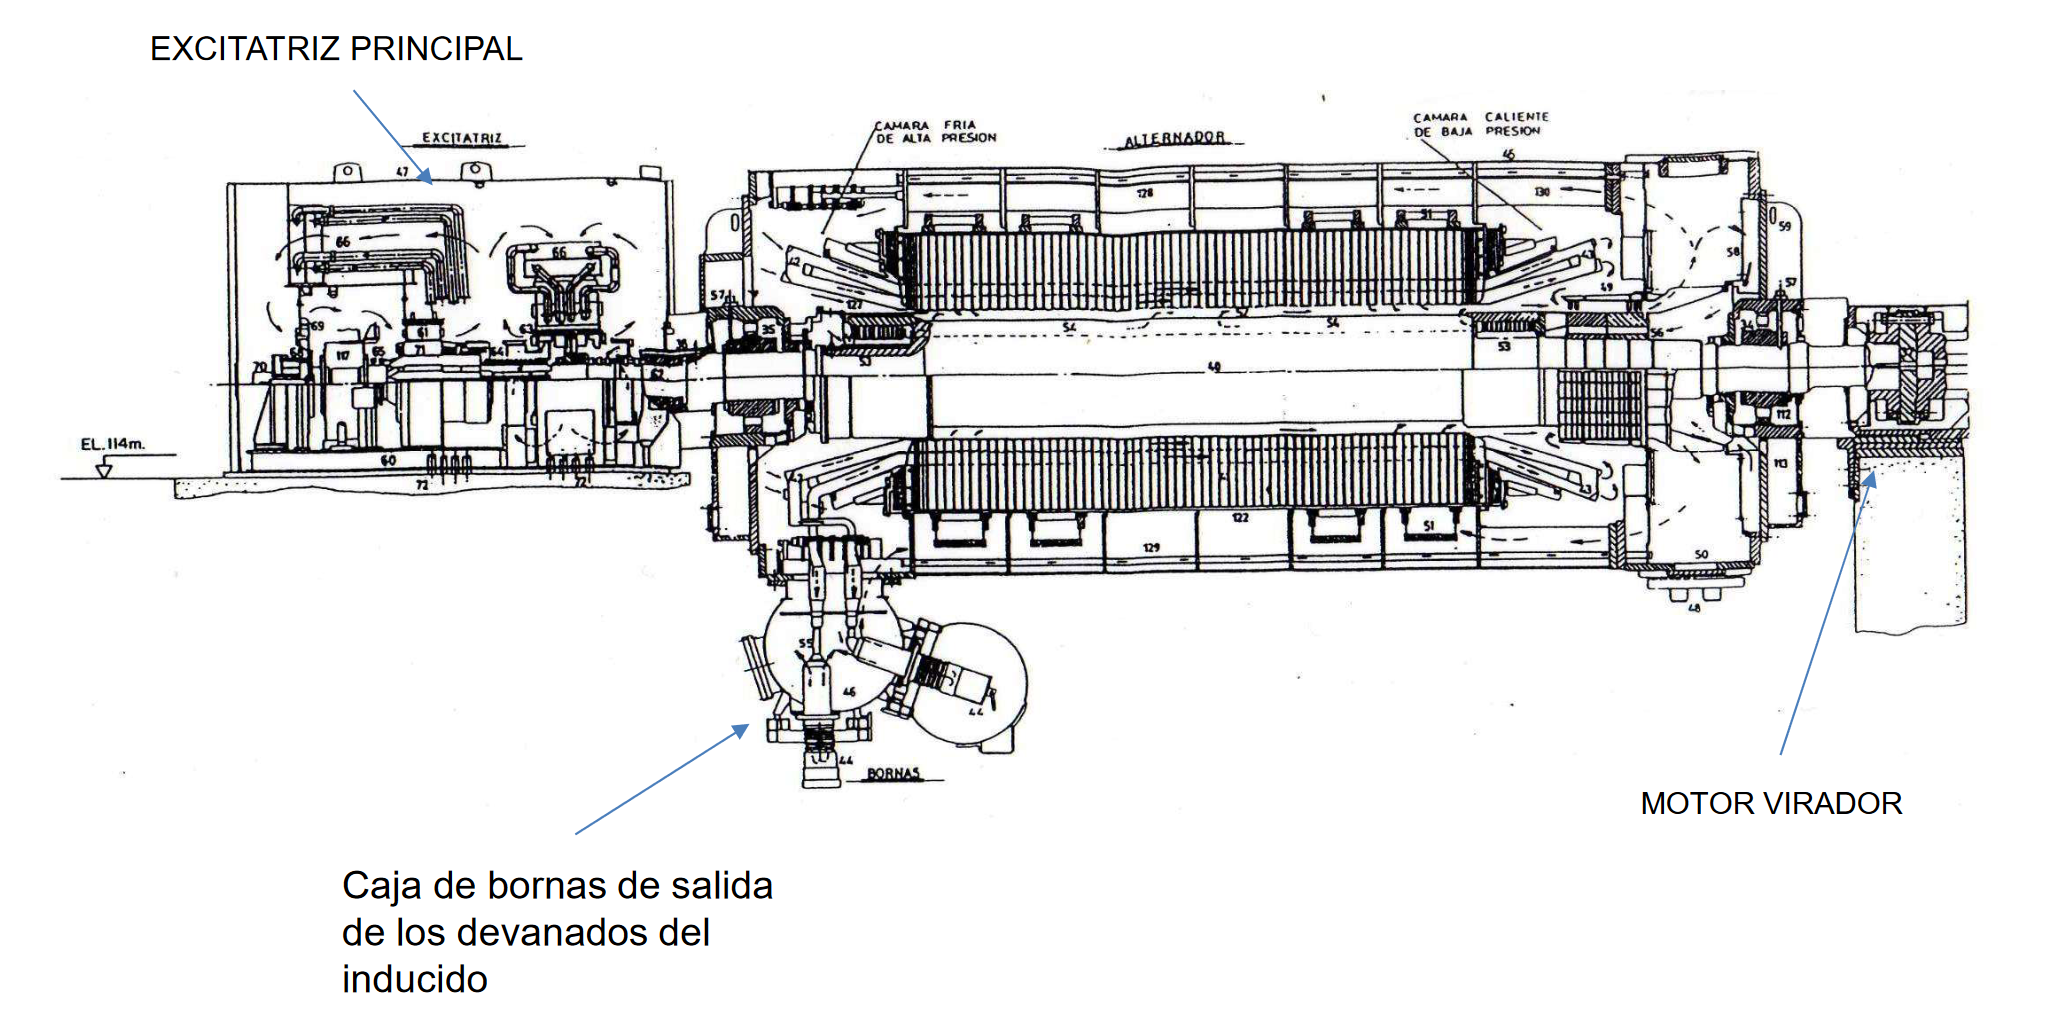
\includegraphics[width=0.9\linewidth]{res/tema6/generador}
			\label{fig:generador}
		\end{figure}
		
		\subsection{Conductores de salida del estátor. Barras de fase aislada.}
			Tienen una capacidad nominal de corriente desde 3 $kA$ hasta 50 $kA$. Se prolongan hasta el bloque interruptor automático + seccionador, bornes de baja tensión del transformador de potencia y el lado
			de alta tensión del transformador de servicios auxiliares. Por su interior circula aire o hidrógeno mediante ventiladores centrífugos. Consta de las siguientes partes:
			
			\begin{itemize}
				\item \textbf{Conductor:} tubo redondo de aluminio extruido de alta conductividad o barras de cobre.
				\item \textbf{Aisladores:} de porcelana o de resina epoxy. Sujetos rígidamente a los tubos de aluminio. Puede haber de uno a cuatro aisladores.
				\item \textbf{Tubo pantalla:} De aluminio. Su misión es doble: servir como conducto para la circulación del refrigerante (hidrógeno o aire) y como apantallamiento para el flujo creado por las altas intensidades. Se ponen a tierra por varios puntos.
			\end{itemize}
		
	\section{Circuito equivalente de un generador síncrono.}
		\subsection{Principio de funcionamiento.}
			En una máquina síncrona las tensiones inducidas forman un sistema trifásico equilibrado y de secuencia directa. Estas tensiones inducidas, si no se consideran efectos de saturación, son proporcionales a la intensidad de excitación en corriente continua, dado que la velocidad de rotación tiene que ser constante para mantener la frecuencia de la red constante.
			
			
			\begin{figure}[H]
				\begin{minipage}{0.5\textwidth}
					\begin{figure}[H]
						\centering
						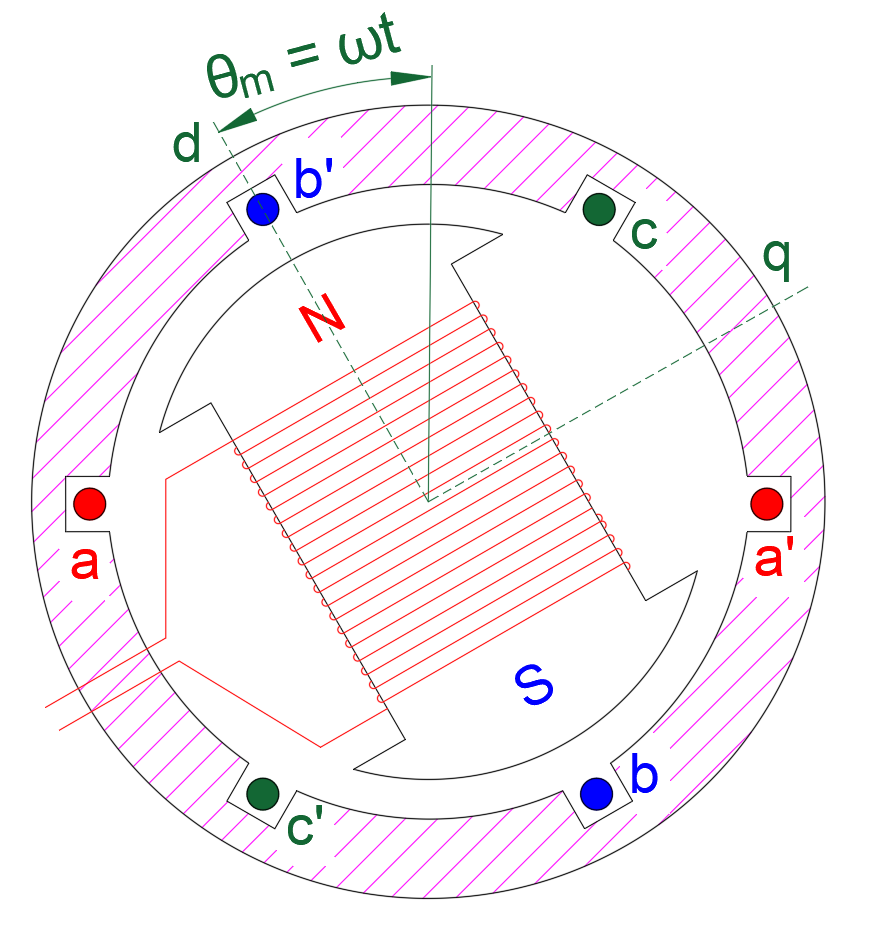
\includegraphics[width=0.7\linewidth]{res/tema6/ejes_dq}
						\label{fig:ejesdq}
					\end{figure}
				\end{minipage}
				\begin{minipage}{0.5\textwidth}
					Si el generador es de polos salientes la reluctancia en el entrehierro no es uniforme y aparecen dos reactancias:
					\begin{itemize}
						\item \textbf{Reactancia del eje directo:} $X_d$.
						\item \textbf{Reactancia del eje transversal o en cuadratura:} $X_q$.
					\end{itemize}
					Si el generador es de rotor cilíndrico sólo se considera la \textbf{reactancia síncrona:} $X_s$.
					
					\[f = \dfrac{p\cdot n}{60} \qquad E = k\cdot \omega \cdot i_{ex}\]
				\end{minipage}
			\end{figure}
			
		\subsection{Circuito equivalente por fase.}
			Considerando un generador de rotor cilíndrico o liso, al conectarla una carga y circular intensidad, estas corrientes crean un campo magnético, denominado \textbf{reacción de inducido}, que presenta una distribución senoidal y que gira a la misma velocidad y en el mismo sentido que el rotor. Esto provoca una caída de tensión en carga respecto de la tensión en vacío, y se representa mediante una reactancia de reacción de inducido, $X_{ri}$.
			
			\begin{figure}[H]
				\begin{minipage}{0.5\textwidth}
					\begin{figure}[H]
						\centering
						\begin{circuitikz}
							\tikzstyle{every node}=[font=\normalsize]
							\draw (3.25,18) to[sinusoidal voltage source, sources/symbol/rotate=auto,l={$\vec E_a$}] (3.25,14.75);
							\draw (3.25,18) to[L,l={$jX_{ri}$} ] (5,18);
							\draw (5,18) to[L,l={$jX_\sigma$} ] (6.75,18);
							\draw (6.75,18) to[R,l={$R$}] (8.5,18);
							\draw [](8.5,18) to[short, -o] (9,18) ;
							\draw [](3.25,14.75) to[short, -o] (9,14.75);
							\draw [->, >=Stealth] (9,17.5) -- (9,15.25)node[pos=0.5,right]{$\vec U_a$};
							\draw [short] (3.5,19) -- (6.5,19)node[pos=0.5,above]{$jX_s$};
							\draw [short] (3.5,19) -- (3.5,18.75);
							\draw [short] (6.5,19) -- (6.5,18.75);
							\draw [->, >=Stealth] (8.25,18) -- (8.75,18)node[pos=0.7,above]{$\vec I_a$};
							\draw [->, >=Stealth] (5,17.5) -- (5,15.25)node[pos=0.5,right]{$\vec E_{ag}$};
						\end{circuitikz}
					\end{figure}
				\end{minipage}
				\begin{minipage}{0.5\textwidth}
					No todo el flujo que crea el inductor es recogido por el inducido. Esta pérdida de flujo se representa mediante una reactancia de dispersión $X_\sigma$.
					
					\[\vec U_a = \vec E_a - \vec I_a(R + jX_{ri} + jX_{\sigma})\]
					\[\Downarrow\]
					\[\vec U_a = \vec E_a - \vec I_a(R + jX_s)\]
					\[\vec U_a = U_a\phase{0^\circ} \qquad \vec E_a = E_a\phase{\delta}\]
				\end{minipage}
			\end{figure}
			
			\begin{figure}[H]
				\begin{minipage}{0.3\textwidth}
					Considerando $R\approx 0$:
					\[P_G = \dfrac{E_a\cdot U_a}{X_S}\cdot \sin \delta\]
					\[Q_G = \dfrac{E_a\cdot U_a \cdot \cos \delta - U_a^2}{X_S}\]
				\end{minipage}
				\begin{minipage}{0.7\textwidth}
					\begin{figure}[H]
						\centering
						\begin{circuitikz}
							\tikzstyle{every node}=[font=\normalsize]
							\draw [ color={rgb,255:red,0; green,0; blue,255}, ->, >=Stealth] (5,14.75) -- (7.75,14.75)node[pos=1,above]{$\vec{U}$};
							\draw [ color={rgb,255:red,255; green,0; blue,0}, ->, >=Stealth] (7.75,14.75) -- (8.5,14)node[pos=1,below]{$R\vec{I}$};
							\draw [ color={rgb,255:red,255; green,0; blue,0}, ->, >=Stealth] (8.5,14) -- (10.5,16.25)node[pos=0.5,right]{$jX_\sigma\vec{I}$};
							\draw [ color={rgb,255:red,0; green,128; blue,0}, ->, >=Stealth] (5,14.75) -- (10.5,16.25)node[pos=0.9,above]{$\vec{E}_{ag}$};
							\draw [ color={rgb,255:red,128; green,0; blue,255}, ->, >=Stealth] (5,14.75) -- (6.25,13.5)node[pos=1,below]{$\vec{I}$};
							\draw [ color={rgb,255:red,210; green,105; blue,0}, ->, >=Stealth] (5,14.75) -- (4,17.75)node[pos=1,right]{$\Phi$};
							\draw [ color={rgb,255:red,255; green,128; blue,0}, ->, >=Stealth] (5,14.75) -- (4.25,17)node[pos=1,right]{$\vec{F}_{r}$};
							\draw [ color={rgb,255:red,255; green,0; blue,128}, ->, >=Stealth] (4.25,17) -- (3,18.25)node[pos=0.8,above]{$\,\,\,\,\vec{F}_i$};
							\draw [ color={rgb,255:red,0; green,128; blue,128}, ->, >=Stealth] (5,14.75) -- (11.75,17.75)node[pos=0.9,above]{$\vec{E}_a$};
							\draw [ color={rgb,255:red,255; green,0; blue,0}, ->, >=Stealth] (10.5,16.25) -- (11.75,17.75)node[pos=0.5,right]{$jX_r\vec{I}$};
							\draw [ color={rgb,255:red,128; green,128; blue,128}, ->, >=Stealth] (5,14.75) -- (2.57,19)node[pos=1,left]{$\Phi_0$};
							\draw [->, >=Stealth] (5,14.75) -- (3,18.25)node[pos=0.9,left]{$\vec{F}_{ex}$};
							\draw (6,14.75) arc [radius=1cm, start angle=0, end angle=-45]node[pos=0.6,right]{$\varphi$};
							\draw (6.5,14.75) arc [radius=1.5cm, start angle=0, end angle=25]node[pos=0.4,right]{$\delta$};
							\draw (7,15.275) arc [radius=2cm, start angle=10, end angle=19]node[pos=0.9,right]{$\delta_m$};
						\end{circuitikz}
					\end{figure}
				\end{minipage}
			\end{figure}
			
			\begin{figure}[H]
				\begin{minipage}{0.65\textwidth}
					\begin{figure}[H]
						\centering
						\begin{circuitikz}[scale = 0.9]
							\tikzstyle{every node}=[font=\normalsize]
							\draw [ color={rgb,255:red,255; green,0; blue,0}, ->, >=Stealth] (10.25,12) -- (14.25,12)node[pos=0.6,below]{$\dfrac{3U_a^2}{X_S}$};
							\draw [->, >=Stealth] (14.25,12) -- (14.25,16.25)node[pos=1,above]{$P\,[MW]$};
							\draw [->, >=Stealth] (14.25,12) -- (17,12)node[pos=1,right]{$Q\,[MV\!A]$};
							\draw [ color={rgb,255:red,0; green,128; blue,255}, ->, >=Stealth] (14.25,12) -- (15.5,14.5)node[pos=0.5,left]{S};
							\draw [ color={rgb,255:red,0; green,128; blue,0}, ->, >=Stealth] (10.25,12) -- (15.5,14.5)node[pos=0.5,above]{$\dfrac{3U_a}{X_S}\cdot E_a$};
							\node [font=\normalsize] at (14.5,11.75) {O};
							\node [font=\normalsize] at (10,11.75) {M};
							\node [font=\normalsize] at (15.25,14.75) {B};
							\node [font=\normalsize] at (15.75,12.25) {A};
							\draw [dashed] (15.5,14.5) -- (15.5,12);
							\draw [dashed] (15.5,14.5) -- (16,15.5);
							\draw [<->, >=Stealth] (14.25,15.25) .. controls (15,15.5) and (15.4,15.25) .. (15.75,15)node[pos=0.5,above]{$\phi$};
							\draw [<->, >=Stealth] (12.75,13.2) .. controls (13,12.75) and (13.1,12.5) .. (13,12)node[pos=0.5,right]{$\delta$};
							\draw [<->, >=Stealth] (16.25,14.5) -- (16.25,12)node[pos=0.5,right]{$P$};
							\draw [short] (15.5,14.5) -- (16.5,14.5);
							\draw [<->, >=Stealth] (14.25,11.25) -- (15.5,11.25)node[pos=0.5,below]{$Q$};
							\draw [ color={rgb,255:red,0; green,128; blue,255}, dashed] (14.25,12) -- (13.25,10.25);
							\draw [ color={rgb,255:red,255; green,128; blue,0}, ->, >=Stealth] (10.25,12) -- (13.25,10.25)node[pos=0.5,below, sloped]{$\dfrac{U_a}{X_S}\cdot I_a$};
							\draw [short] (14.25,11) -- (14.25,12);
							\draw [short] (15.5,11) -- (15.5,12);
							\node at (10.25,12) [circ] {};
							\node at (14.25,12) [circ] {};
							\node at (15.5,14.5) [circ] {};
							\node at (15.5,12) [circ] {};
						\end{circuitikz}
						
						\label{fig:my_label}
					\end{figure}
				\end{minipage}
				\begin{minipage}{0.35\textwidth}
					Se pueden obtener los valores de P y Q multiplicando escalarmente todos los vectores por $\dfrac{U_a}{X_S}$, si consideramos despreciable la $R$. Será útil a la hora de dibujar el diagrama de capacidad de la máquina.
					\[P = 3\cdot U_a \cdot I_a \cdot \cos \phi\]
					\[Q = 3\cdot U_a \cdot I_a \cdot \sin \phi\]
				\end{minipage}
			\end{figure}
			
		\subsection{Modelo fasorial para un generador de polos salientes.}
			\begin{figure}[H]
				\centering
					\begin{circuitikz}
						\tikzstyle{every node}=[font=\normalsize]
						\draw [ color={rgb,255:red,255; green,0; blue,0}, ->, >=Stealth] (10.25,12) -- (16,12)node[pos=0.85,below]{$\vec U_a$};
						\draw [ color={rgb,255:red,0; green,128; blue,0}, ->, >=Stealth] (10.25,12) -- (19.25,13.5)node[pos=0.5,above]{$\vec{E}_a$};
						\node [font=\normalsize] at (10,12.25) {O};
						\draw [<->, >=Stealth] (14.75,12.75) .. controls (14.85,12.5) and (14.85,12.25) .. (14.75,12)node[pos=0.5,right]{$\delta$};
						\node at (10.25,12) [circ] {};
						\draw [ color={rgb,255:red,255; green,128; blue,0}, ->, >=Stealth] (16,12) -- (16.75,11.5)node[pos=0.5,above, sloped]{$R\vec I_a$};
						\draw [<->, >=Stealth] (12.75,12) .. controls (12.75,11.5) and (12.75,11.25) .. (12.5,10.75)node[pos=0.5,right]{$\varphi$};						
						\draw [ color={rgb,255:red,0; green,128; blue,255}, ->, >=Stealth] (10.25,12) -- (10.75,9.75)node[pos=0.5,right]{$\vec I_{ad}$};
						\draw [ color={rgb,255:red,0; green,128; blue,255}, ->, >=Stealth] (10.25,12) -- (13,12.45)node[pos=0.5,above, sloped]{$\vec I_{aq}$};
						\draw [dashed] (13,12.45) -- (13.5,10.25);
						\draw [dashed] (10.75,9.75) -- (13.5,10.25);
						\draw [ color={rgb,255:red,0; green,128; blue,255}, ->, >=Stealth] (19.5,12) -- (19.25,13.5)node[pos=0.5,right]{$jX_q \vec I_{aq}$};
						\draw [ color={rgb,255:red,0; green,128; blue,255}, ->, >=Stealth] (16.75,11.5) -- (19.5,12)node[pos=0.5,above, sloped]{$jX_d \vec I_{ad}$};
						\draw [ color={rgb,255:red,255; green,128; blue,0}, ->, >=Stealth] (10.25,12) -- (13.5,10.25)node[pos=0.5,above]{$\vec I_a$};
						\draw [ color={rgb,255:red,0; green,128; blue,255}, dashed] (10.25,12) -- (9.75,14.25)node[pos=1,right]{d};
						\draw [ color={rgb,255:red,0; green,128; blue,255}, dashed] (19.25,13.5) -- (20.75,13.75)node[pos=1,above]{q};
					\end{circuitikz}
				
				\label{fig:my_label}
			\end{figure}
			
			Recordar que $d \perp q$. Se suele considerar $X_S = \dfrac{X_d + X_q}{2}$
			\[\vec U_a = \vec E_a - R\vec I_a - jX_d \vec I_{ad} - jX_q \vec I_{aq} \quad \Rightarrow \quad \vec U_a = \vec E_a - R\vec I_a - j(X_d - X_q)\vec I_{ad} - jX_q \vec I_a\]
			
			
			El vector $j(X_d - X_q)\vec I_{ad}$ está en fase con $\vec E_a$.
			
			\[P_G = \dfrac{U_a E_a}{X_d} \sen \delta + \dfrac{U_a^2}{2}\left(\dfrac{1}{X_q} - \dfrac{1}{X_d}\right)\sin 2\delta\]
			\[Q_G = \dfrac{U_a E_a}{X_d} \cos \delta - U_a^2\left(\dfrac{\sin^2 \delta}{X_q} + \dfrac{\cos^2 \delta}{X_d}\right)\]
			
		\subsection{Determinación de la reactancia síncrona saturada.}
			Se obtiene a través de ensayos de vacío y cortocircuito, utilizando sus curvas características. La impedancia saturada da resultados más precisos que la no saturada.
			\[Z_{s0} = f(E_0)\equiv f(I_e) \quad \because E_0 = f(I_e)\]
			\[Z_{s0} = \dfrac{U_N}{I_{cc0}}\qquad X_S = \sqrt{Z_S^2 - R^2}\]
			
		\subsection{Estabilidad.}
		\vspace{-1.5cm}
			\begin{figure}[H]
				\begin{minipage}{0.5\textwidth}
					\begin{figure}[H]
						\centering
						\begin{circuitikz}[scale = 1.1]
							\tikzstyle{every node}=[font=\normalsize]
							\draw [->, >=Stealth] (11,11.75) -- (15.75,11.75)node[pos=1,right]{$\delta$};
							\draw [->, >=Stealth] (11,11.75) -- (11,16)node[pos=1,right]{P};
							\draw [color={rgb,255:red,255; green,0; blue,0},short] (11,11.75) .. controls (12.75,17.25) and (13.5,17) .. (15.25,11.75);
							\node [font=\normalsize] at (15.25,11.5) {$180^\circ$};
							\draw [dashed] (11,14.75) -- (15.5,14.75)node[pos=0,left]{$P_m$};
							\draw [dashed] (11,13.25) -- (15.5,13.25)node[pos=0,left]{$P_0$};
							\draw [short] (11.5,13.25) -- (11.5,14.75);
							\draw [short] (11.5,14.75) -- (12.75,14.75);
							\draw [short] (12.75,14.75) -- (12.75,15.65);
							\node [font=\normalsize] at (11.75,14.5) {A1};
							\node [font=\normalsize] at (12.5,15) {A2};
							\draw [dashed] (11.5,13.25) -- (11.5,11.75)node[pos=1,below]{$\delta_{0}$};
							\draw [dashed] (12.75,14.75) -- (12.75,11.75)node[pos=1,below]{$\delta_{max}$};
							\draw [dashed] (12.125,14.75) -- (12.125,11.75)node[pos=1,below]{$\delta_m$};
						\end{circuitikz}
						
						\label{fig:my_label}
					\end{figure}
				\end{minipage}
				\begin{minipage}{0.5\textwidth}
					Límite de estabilidad: $\delta = 90^\circ$.
					
					
					\textbf{Estabilidad transitoria:} Ante un cambio del ángulo del par provocado por un cambio brusco de potencia activa en la red, se produce un proceso oscilante de aceleración y deceleración, que se va amortiguando en un tiempo que depende de la inercia de las masas en rotación de la unidad de generación, turbina y generador. Durante este proceso, el generador pierde la sincronización con la red y aparecen sobreintensidades en las líneas.
				\end{minipage}
			\end{figure}
			
			Si las áreas formadas de aceleración (A1) y deceleración (A2) son iguales se consigue la estabilización en un nuevo valor de ángulo y P. En caso contrario, el sistema se vuelve inestable y hay que desacoplar el generador de la red.
			
		\subsection{Comportamiento conectado a la red eléctrica.}
			\vspace{-0.5cm}
			\begin{figure}[H]
				\begin{minipage}{0.5\textwidth}
					Se supone que la potencia nominal de la máquina es pequeña con relación al resto del sistema. A este nudo se le denomina nudo de potencia infinita. Se consideran $X_S$ de la máquina y $U_{red}$ constantes.
				\end{minipage}
				\begin{minipage}{0.5\textwidth}
					\begin{figure}[H]
						\centering
						\begin{circuitikz}
							\tikzstyle{every node}=[font=\normalsize]
							\draw (11.5,14) to[sinusoidal voltage source, sources/symbol/rotate=auto,l={ \normalsize $\vec U_p$}] (11.5,12);
							\draw (11.5,14) to[L,l={ \normalsize $X_S$} ] (14.25,14);
							\draw (14.25,14) to[sinusoidal voltage source, sources/symbol/rotate=auto,l={ \normalsize $\vec U_{red}$}] (14.25,12);
							\draw (11.5,12) to (11.5,11.75) node[ground]{};
							\draw (14.25,12) to (14.25,11.75) node[ground]{};
							\draw [->, >=Stealth] (13.5,14) -- (14,14)node[pos=0.5,above]{$\vec I_p$};
						\end{circuitikz}
						
						\label{fig:my_label}
					\end{figure}
				\end{minipage}
			\end{figure}
			
	\section{Diagrama límite de capacidad de la máquina síncrona.}
		El campo de funcionamiento posible de la máquina cuando está acoplada a una red de potencia infinita queda limitado por los siguientes límites:
		\begin{itemize}
			\item \textbf{Límite térmico del inducido:} $I_{max}$. La corriente máxima que el inducido puede dar teniendo en cuenta su calentamiento admisible. Si se considera la tensión en bornes constante el límite térmico se puede establecer como una $S_{max}$.
			
			\item \textbf{Límite de tensión interna máxima:} $E_{max}$. Definida por la intensidad máxima de excitación que puede recorrer el rotor y/o la máxima tensión de aislamiento. Suele ser $2.1 p.u.$
			
			\item \textbf{Límites de la potencia mecánica:} $P_{max},\,P_{min}$. Establecidas por las potencias máxima y mínima que puede dar/necesita la turbina.
			
			\item \textbf{Límite de estabilidad:} $\delta_{max}$. Se establece a partir del apartado anterior. El $\delta_{max}$ práctico suele estar en torno a $80^\circ$.
		\end{itemize}
			
		\begin{figure}[H]
			\centering
			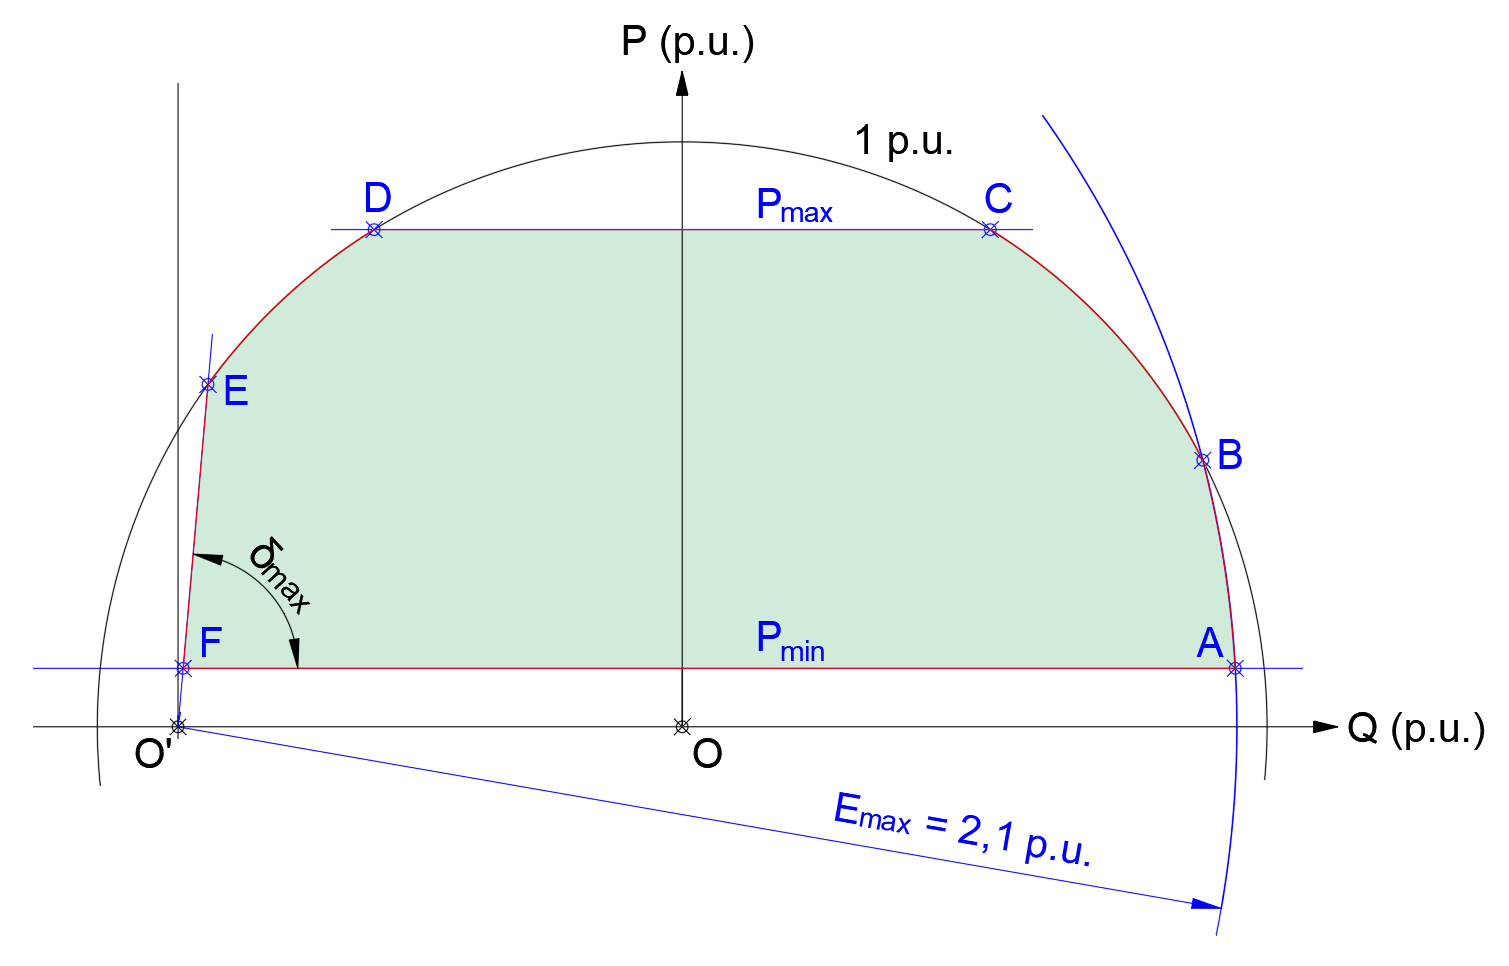
\includegraphics[width=0.8\linewidth]{res/tema6/diagramaCapacidad}
			\label{fig:diagramacapacidad}
		\end{figure}
		
	\section{Modos de funcionamiento de una máquina síncrona.}
		\begin{table}[H]
			\centering
			\renewcommand{\arraystretch}{1.1}
			\begin{tabular}{ccccl}
				\textbf{Caso} & \textbf{Finalidad} & \textbf{Constantes} & \textbf{Variables} & \textbf{Consecuencias}\\
				\hline
				\multirow{3}{*}{1} & \multirow{3}{*}{Variar $P$}   & \multirow{3}{*}{$I_{ex}$}  & \multirow{3}{*}{$P_{mec}$}  & $\Phi = cte \Rightarrow E_0 = cte \Rightarrow n = cte$ \\
				&              &           &            & $\updownarrow\delta\Rightarrow\updownarrow jX_S\vec{I}_a\Rightarrow\updownarrow P_a$ \\
				&              &           &            & $\uparrow\delta \Rightarrow\uparrow P\text{ y }\downarrow Q$ \\\hline
				\multirow{6}{*}{2} & \multirow{6}{*}{Variar $Q$}   & \multirow{6}{*}{$P_{mec}$} & \multirow{6}{*}{$I_{ex}$}   & $\updownarrow E_a$ \\
				&              &           &            & $Proy_P(jX_s\vec{I}_a) = cte$ \\
				&              &           &            & $Proy_Q(jX_s\vec{I}_a)$: \\
				&              &           &            & $\quad\text{Sobreexcitada, inductivo}$ \\
				&              &           &            & $\quad\text{Subexcitada, capacitivo}$ \\
				&              &           &            & $\quad\cos{\varphi} = 1$ \\\hline
				\multirow{3}{*}{3} & \multirow{3}{*}{Asincronismo} & \multirow{3}{*}{$P_{mec}$} & \multirow{3}{*}{$I_{ex}$}   & La red aporta la magnetización de la máquina $\Rightarrow$ \\
				&              &           &            & sobreintensidades en el inducido. \\
				&              &           &            & Aporta $P$, consume $Q$ \\\hline
				\multirow{3}{*}{4} & \multirow{3}{*}{\parbox{2cm}{\centering Oscilaciones\\pendulares}} & \multirow{3}{*}{$I_{ex}$}  & \multirow{3}{*}{\parbox{2cm}{\centering C. bruscos\\$P_{mec}$}} & Pérdida de la sicronización con la red. \\
				&              &           &   & Sobreintensidades en las líneas. \\
				&              &           &            & \textuparrow Inercia \textrightarrow \textuparrow Tiempo de oscilación\\\hline
				\multirow{2}{*}{5} & Compensador  & \multirow{2}{*}{$I_{ex}$}  & \multirow{2}{*}{$P_{mec}$}  & Consumo de $P_{mec}$ por pérdida de par en el eje. \\
				& síncrono     & 			 & 			  & Consume activa, consume o aporta reactiva.\\\hline
			\end{tabular}
			\label{tab:modosFunc}
		\end{table}
		
		\begin{figure}[H]
			\begin{minipage}{0.5\textwidth}
				\begin{figure}[H]
					\centering
					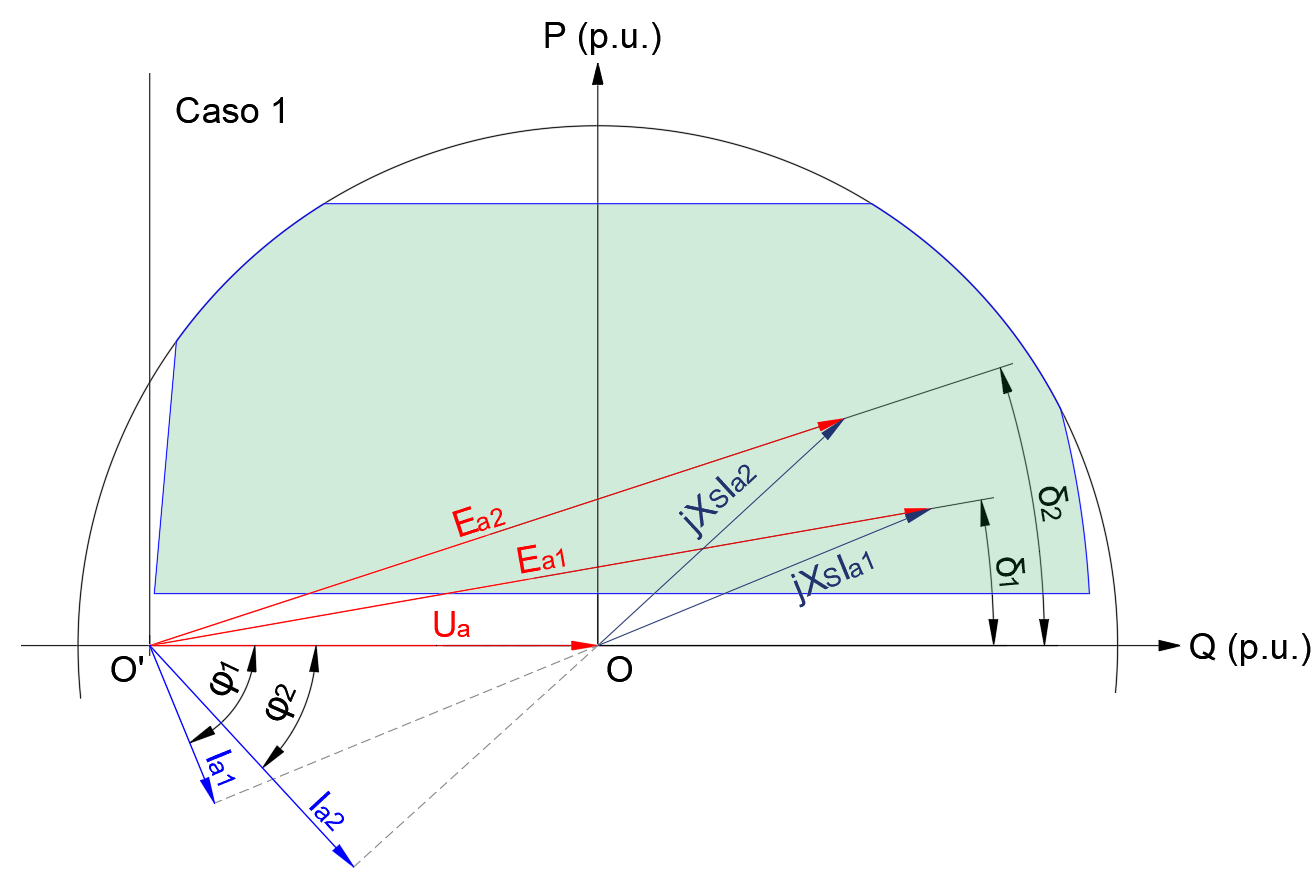
\includegraphics[width=1\linewidth]{res/tema6/modoFunc1}
					\label{fig:modofunc1}
				\end{figure}
			\end{minipage}
			\begin{minipage}{0.5\textwidth}
				\begin{figure}[H]
					\centering
					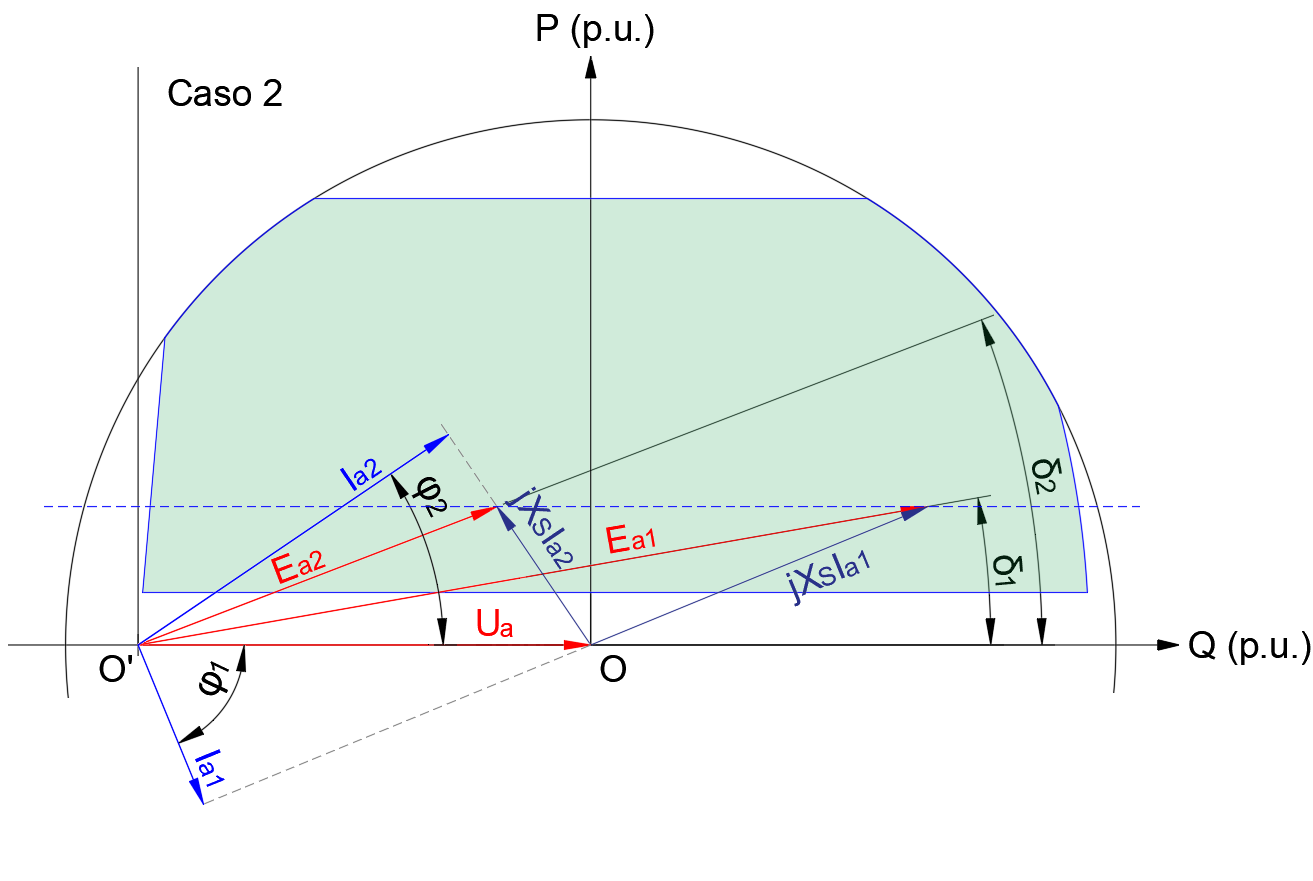
\includegraphics[width=1\linewidth]{res/tema6/modoFunc2}
					\label{fig:modofunc2}
				\end{figure}
			\end{minipage}
		\end{figure}
		
		
	\section{Ejercicio completo resuelto.}		
		Un alternador de polos salientes de una central hidráulica tiene las siguientes características técnicas:
		\begin{figure}[H]
			\begin{minipage}{0.33\textwidth}
				\begin{itemize}
					\item $S_n = 300\,MV\!A$
					\item $U_n = 22\,kV$
					\item $\cos \varphi_n = 0.85\,ind$
					\item $p = 20$
				\end{itemize}
			\end{minipage}
			\begin{minipage}{0.33\textwidth}
				\begin{itemize}
					\item $\delta_{max} = 85^\circ$
					\item $X_d = 2.45\,\varOmega/fase$
					\item $X_q = 1.45\,\varOmega/fase$
				\end{itemize}
			\end{minipage}
			\begin{minipage}{0.33\textwidth}
				\begin{itemize}
					\item $E_{\text{\textit{exc, máx}}} = 2.1\,p.u.$
					\item $P_{max} = 255\,MW$
					\item $P_{min} = 45\,MW$
				\end{itemize}
			\end{minipage}
		\end{figure}
		

		Dibujar el diagrama de capacidad en valores $p.u.$ y calcular los valores de $P\,[MW]$, $Q\,[MV\!Ar]$, $S\,[MV\!A]$, $I\,[kA]$, $\cos \varphi$, $E\,[kV]$ y $\delta$ para cada punto de intersección entre valores límites. Considerar despresciable la caída de tensión en los devanados del inducido por la resistencia 
		interna.
		
		
		\noindent\makebox[\linewidth]{\rule{\paperwidth}{0.4pt}}
		\vspace{-0.2cm}
		
		
		$S_n = S_b = 1\,p.u.\qquad U_n = U_b = 1\,p.u.$
		
		\vspace{0.1cm}
		$I_n = \dfrac{S_b}{\sqrt{3}U_b} = \dfrac{300\cdot 10^6}{\sqrt{3}\cdot 22\cdot 10^3} = 7.87\,kA = I_b$
		
		\vspace{0.1cm}
		$Z_b = \dfrac{U_b^2}{S_b} = \dfrac{(22\cdot 10^3)^2}{300\cdot 10^6} = 1.61\,\varOmega$
		
		\vspace{0.1cm}
		$X_s = \dfrac{X_d + X_q}{2} = \dfrac{2.45 + 1.45}{2} = 1.95\,\varOmega/fase\quad \Rightarrow \quad X_{s,\,p.u.} = \dfrac{X_s}{Z_b} = 1.21\,p.u.$
		
		\vspace{0.1cm}
		Límite inductor $=\dfrac{E\cdot U_n}{X_{s,\,p.u.}} = \dfrac{2.1\cdot 1}{1.21} = 1.7355\,p.u.$
		
		\vspace{0.1cm}
		$P_{max,\,p.u.} = \dfrac{255}{300} = 0.85\,p.u.\qquad P_{min,\,p.u.} = \dfrac{45}{300} = 0.15\,p.u.$
		
		\subsubsection*{Punto A.}
			Datos conocidos: $P_{min} = 0.15\,p.u.\quad E_{max} = 2.1\,p.u.\quad X_s = 1.21\,p.u.\quad U = 1\,p.u.$
			
			\vspace{0.1cm}
			$P_A = \dfrac{E\cdot U}{X_s}\cdot \sin \delta = 0.15 \quad \Rightarrow \quad \delta = 4.95^\circ$
			
			\vspace{0.1cm}
			$Q_A = \dfrac{E\cdot U}{X_s}\cdot \cos \delta - \dfrac{U^2}{X_s} = 0.9\,p.u.\cdot S_b = 271.08\,MV\!Ar$
			
			\vspace{0.1cm}
			$S_A = \sqrt{P_A^2+Q_A^2} = 0.92\cdot S_b = 276\,MV\!A$
			
			\vspace{0.1cm}
			$I_A = \dfrac{S_A}{\sqrt{3}\cdot U_A} = \dfrac{276\cdot 10^6}{\sqrt{3}\cdot 22\cdot 10^3} = 7.2\,kA$
			
			\vspace{0.1cm}
			$\varphi_A = \arctan \left(\dfrac{Q_A}{P_A}\right) = 80.57^\circ \quad \Rightarrow \quad \cos \varphi_A = 0.16$
		
		\subsubsection*{Punto B.}
			Datos conocidos: $S_n = 1\,p.u.\quad U_n = 1\,p.u.\quad X_s = 1.21\,p.u.\quad E_{max} = 2.1\,p.u.$
			
			\vspace{0.1cm}
			$
			\left.
			\begin{matrix}
				P_B = \dfrac{E_0\cdot U}{X_s}\cdot \sin \delta\\
				Q_B = \dfrac{E_0\cdot U}{X_s}\cdot \cos \delta - \dfrac{U^2}{X_s}\\\\
				S^2 = P^2 + Q^2
			\end{matrix}
			\right\}
			\left(\dfrac{E_0\cdot U}{X_s}\sin \delta\right)^2 + \left(\dfrac{E_0\cdot U}{X_s}\cos \delta - \dfrac{U^2}{X_s}\right)^2 = 1
			$
			
			\vspace{0.1cm}
			Resolviendo se obtiene $\cos \delta = 0.93 \quad \Rightarrow \quad \delta_B = 20^\circ$
			
			\vspace{0.1cm}
			$P_B = \dfrac{2.1\cdot 1}{1.21}\sin 20^\circ = 0.59\,p.u. \cdot S_b = 177.45\,MW$
			
			\vspace{0.1cm}
			$Q_B = \dfrac{2.1\cdot 1}{1.21}\cos 20^\circ - \dfrac{1^2}{1.21} = 0.81\,p.u.\cdot S_b = 241.89\,MV\!Ar$
			
			\vspace{0.1cm}
			$\varphi_B = \arctan\left(\dfrac{Q_B}{P_D}\right) = 53.74^\circ \quad \Rightarrow \quad \cos \varphi_B = 0.59$
			
			\vspace{0.1cm}
			$I_B = I_n = 7.87\,kA$
			
		\subsubsection*{Punto C.}
			Datos conocidos: $P_{max} = 0.85\,p.u.\quad S_n = 1\,p.u.\quad I_n = 7.87\,kA$
			
			\vspace{0.1cm}
			$Q_C = \sqrt{S^2 - P^2} = \sqrt{1^2 - 0.85^2} = 0.527\,p.u. = 158.03\,MV\!A$
			
			\vspace{0.1cm}
			$\tan \varphi_C = \dfrac{Q_C}{P_C} = \dfrac{158.03}{255} = 0.619 \quad \Rightarrow \quad \varphi_C = 31.78^\circ \quad \Rightarrow \quad \cos \varphi_C = 0.85$
			
			\vspace{0.1cm}
			$P_C = \dfrac{E_0\cdot U}{X_s}\sin \delta = 0.85\,p.u. \quad \Rightarrow \quad E_C = \dfrac{P_C \cdot X_S}{U\cdot \sin \delta}$
			
			\vspace{0.1cm}
			Sustituyendo en $Q_C = \dfrac{E_0\cdot U}{X_s}\cdot \cos \delta - \dfrac{U^2}{X_s} = \dfrac{\dfrac{P_C\cdot X_s}{U\cdot \sin \delta}}{X_s}\cos \delta - \dfrac{U^2}{X_s} = \dfrac{P_C}{\sin \delta}\cos \delta - \dfrac{U^2}{X_s} = 0.527$
			
			\vspace{0.1cm}
			$\dfrac{0.85}{\sin \delta}\cos \delta - \dfrac{1}{1.21} = 0.527 \quad \Rightarrow \quad \dfrac{0.85}{\tan \delta} = 1.350 \quad \Rightarrow \quad \tan \delta = 0.628 \quad \Rightarrow \quad \delta_C = 32.129^\circ$
			
			\vspace{0.1cm}
			$E_C = \dfrac{0.85\cdot 1.21}{1\cdot \sin 32.12^\circ} = 1.933\,p.u. = 42.54\,kV$
			
		\subsubsection*{Punto D.}
			Datos conocidos: $P_{max} = 0.85\,p.u.\quad S_n = 1\,p.u.\quad I_n = 7.87\,kA$
			
			\vspace{0.1cm}
			$Q_D = \sqrt{S^2 - P^2} = -0.527 = -158.03\,MV\!Ar$
			
			\vspace{0.1cm}
			$\tan \varphi_D = \dfrac{Q_D}{P_D} = \dfrac{-158.03\,MV\!Ar}{255\,MW} = -0.619 \quad \Rightarrow \quad \varphi_D = -31.78^\circ \quad \Rightarrow \quad \cos \varphi_D = 0.85$ (cap)
			
			\vspace{0.1cm}
			$P_D = \dfrac{E_0\cdot U}{X_s}\sin \delta = 0.85\,p.u. \quad \Rightarrow \quad E_D = \dfrac{P_D \cdot X_s}{U\cdot \sin \delta}$
			
			\vspace{0.1cm}
			Sustituyendo en $Q_D = \dfrac{E_0\cdot U}{X_s}\cdot \cos \delta - \dfrac{U^2}{X_s} = \dfrac{\dfrac{P_C\cdot X_s}{U\cdot \sin \delta}}{X_s}\cos \delta - \dfrac{U^2}{X_s} = \dfrac{P_D}{\sin \delta}\cos \delta - \dfrac{U^2}{X_s} = -0.527$
			
			\vspace{0.1cm}
			Operando se obtiene $\tan \delta = 2.83 \quad \Rightarrow \quad \delta = 70.59^\circ$
			
			\vspace{0.1cm}
			$E_D = \dfrac{0.85\cdot 1.21}{1\cdot \sin 70.59^\circ} = 1.09 = 23.99\,kV$
		
		\subsubsection*{Punto E.}
			Datos conocidos: $S_n = 1\,p.u.\quad I_n = 7.87\,kA\quad \delta_{max} = 85^\circ$
			
			\vspace{0.1cm}
			$
			\left.
			\begin{matrix}
				P_E = \dfrac{E_0\cdot U}{X_s}\cdot \sin \delta\\
				Q_E = \dfrac{E_0\cdot U}{X_s}\cdot \cos \delta - \dfrac{U^2}{X_s}\\\\
				S^2 = P^2 + Q^2
			\end{matrix}
			\right\}
			\left(\dfrac{E_0\cdot U}{X_s}\sin \delta\right)^2 + \left(\dfrac{E_0\cdot U}{X_s}\cos \delta - \dfrac{U^2}{X_s}\right)^2 = 1
			$
			
			\vspace{0.1cm}
			Resolviendo: $0.68E^2 - 0.119E - 0.318 = 0 \quad \Rightarrow \quad E_E = 0.77 = 16.98\,kV$
			
			\vspace{0.1cm}
			$P_E = \dfrac{0.77\cdot 1}{1.21}\sin 85^\circ = 0.634 = 190.18\,MW$
			
			\vspace{0.1cm}
			$Q_E = \dfrac{0.77\cdot 1}{1.21}\cos 85^\circ - \dfrac{1^2}{1.21} = -0.77 = -231.3\,MV\!Ar$
			
			\vspace{0.1cm}
			$\tan \varphi = \dfrac{Q_E}{P_E} = 1.22 \quad \Rightarrow \quad \varphi_E = -50.57^\circ \quad \Rightarrow \quad \cos \varphi_E = 0.63$ (cap)
		
		\subsubsection*{Punto F.}
			Datos conocidos: $P_{min} = 0.15\,p.u.\quad \delta_{max} = 85^\circ\quad X_s = 1.21\,p.u.$
			
			\vspace{0.1cm}
			$P_F = \dfrac{E_0\cdot U}{X_s}\cdot \sin \delta = 0.15 \quad \Rightarrow \quad E_F = 0.182\,p.u. = 4.01\,kV$
			
			\vspace{0.1cm}
			$Q_F = \dfrac{0.182\cdot 1}{1.21}\cos 85^\circ - \dfrac{1^2}{1.21} = -0.813 = -244.0\,MV\!Ar$
			
			\vspace{0.1cm}
			$S_F = \sqrt{P_F^2 + Q_F^2} = 0.826\,p.u. = 248.02\,MV\!A \qquad I_F = \dfrac{S_F}{\sqrt{3}\cdot U_n} = 6.51\,kA$
			
			\vspace{0.1cm}
			$\tan \varphi_F = \dfrac{Q_F}{P_F} = 5.422 \quad \Rightarrow \quad \varphi_F = -79.55^\circ \quad \Rightarrow \quad \cos \varphi_F = 0.181$ (cap)
		
			
		
		\chapter{Esquema TT. Protección diferencial}
\section{Análisis del esquema TT}
En este esquema están conectados a tierra tanto el centro de la estrella del transformador como las masas. Se produce un defecto fase-tierra con tierra de retorno.
\begin{figure}[H]
	\centering
	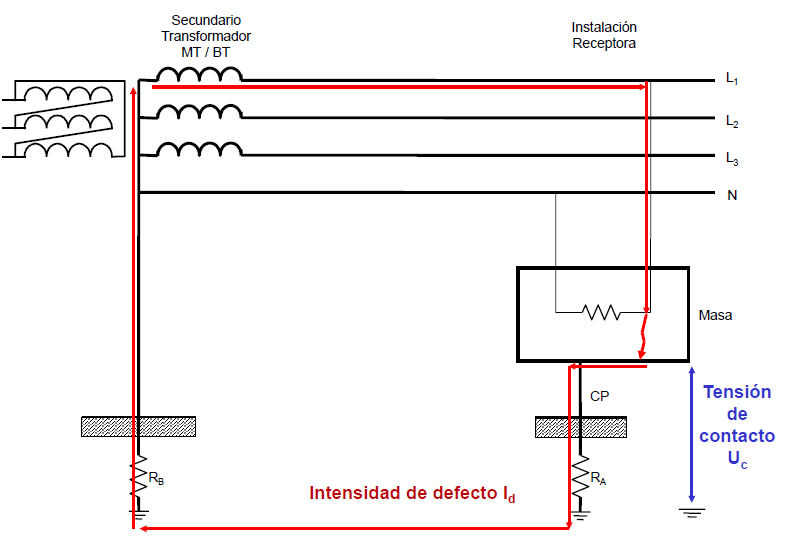
\includegraphics[width=0.5\linewidth]{Images/26}
	\label{fig:26}
\end{figure}

Su circuito equivalente es:
\begin{figure}[H]
	\centering
	\begin{adjustbox}{width=1\textwidth}
	
		\begin{circuitikz}
			\tikzstyle{every node}=[font=\normalsize]
			\draw (5.25,14.25) to[sinusoidal voltage source, sources/symbol/rotate=auto,l={ \normalsize $cU_{\text{fase-neutro}}$}] (5.25,11.25);
			\draw (6,15.5) to[european resistor,l={ \normalsize $\dfrac{2}{3} Z_{\text{media tension}}$}] (11,15.5);
			\draw (5.25,14.25) to[short] (5.25,15.5);
			\draw (5.25,15.5) to[short] (6.25,15.5);
			\draw (11,15.5) to[european resistor,l={ \normalsize $Z_{\text{trafo}}$}] (13.5,15.5);
			\draw (13.5,15.5) to[european resistor,l={ \normalsize $R_{\text{línea}}$}] (15.5,15.5);
			\draw (15.5,15.5) to[european resistor,l={ \normalsize $R_{\text{defecto}}$}] (15.5,12.75);
			\draw (15.5,12.75) to[european resistor,l={ \normalsize $R_{\text{cable protección}}$}] (15.5,10.75);
			\draw (15.5,10.75) to[european resistor,l={ \normalsize $R_{\text{puesta a tierra masas utilización}}$}] (15.5,8.5);
			\draw (5.25,11.25) to[european resistor,l={ \normalsize $R_{\text{puesta a tierra neutro}}$}] (5.25,8.5);
			\draw (5.25,8.5) to (5.25,8.25) node[ground]{};
			\draw (15.5,8.5) to (15.5,8.25) node[ground]{};
			\draw [ color={rgb,255:red,200; green,0; blue,255}, <->, >=Stealth] (14.25,13) -- (14.25,7.75)node[pos=0.5, fill=white]{$U_{contacto}$};
			\draw [ color={rgb,255:red,200; green,0; blue,255}, ->, >=Stealth] (8.5,14.75) -- (12.5,14.75)node[pos=0.5, fill=white]{$I_{defecto}$};
			\node [font=\normalsize, color={rgb,255:red,200; green,0; blue,255}] at (8.5,16.25) {$Z_{MT}$};
			\node [font=\normalsize, color={rgb,255:red,200; green,0; blue,255}] at (12.25,16.25) {$Z_T$};
			\node [font=\normalsize, color={rgb,255:red,200; green,0; blue,255}] at (14.5,16.25) {$R_F$};
			\node [font=\normalsize, color={rgb,255:red,200; green,0; blue,255}] at (16.5,14.5) {$R_d$};
			\node [font=\normalsize, color={rgb,255:red,200; green,0; blue,255}] at (16.5,12.25) {$R_{CP}$};
			\node [font=\normalsize, color={rgb,255:red,200; green,0; blue,255}] at (16.5,10) {$R_A$};
			\node [font=\normalsize, color={rgb,255:red,200; green,0; blue,255}] at (6.5,10.25) {$R_B$};
			\node [font=\normalsize, color={rgb,255:red,200; green,0; blue,255}] at (6.5,13.25) {$cU_0$};
		\end{circuitikz}
	\end{adjustbox}
	\label{fig:my_label}
\end{figure}

En estas condiciones:
\begin{equation}
	Z_{bucle}=\dfrac{2}{3}Z_{MT}+Z_T+Z_F+R_d+R_{CP}+R_A+R_B
\end{equation}
\begin{equation}
	I_d=\dfrac{c U_0}{Z_{bucle}}
\end{equation}
\begin{equation}
	U_c=\left(R_{CP}+R_A\right)I_d
\end{equation}
\subsection{Circuito equivalente simplificado en caso de fallo}
Normalmente las resistencias de puesta a tierra son mayores que el resto de impedancias:
\begin{equation}
	R_B+R'_A \ggg \dfrac{2}{3}Z_{MT}+Z_T+Z_F+R_d
\end{equation}

El caso más desfavorable desde el punto de vista de la protección:
\begin{equation}
	R_d=0
\end{equation}

La resistencia desde la masa de utilización a tierra:
\begin{equation}
	R_A'=R_A+R_{CP}
\end{equation}
\begin{center}
	\begin{figure}[H]
		\centering
	\begin{adjustbox}{width=0.5\textwidth}
		
		\begin{circuitikz}
			\tikzstyle{every node}=[font=\normalsize]
			\draw (5.25,14.25) to[sinusoidal voltage source, sources/symbol/rotate=auto,l={ \normalsize $cU_0$}] (5.25,11.25);
			\draw (5.25,14.25) to[short] (5.25,15.5);
			\draw (5.25,15.5) to[short] (6.25,15.5);
			\draw (15.5,10.75) to[european resistor] (15.5,8.5);
			\draw (5.25,11.25) to[european resistor] (5.25,8.5);
			\draw (5.25,8.5) to (5.25,8.25) node[ground]{};
			\draw (15.5,8.5) to (15.5,8.25) node[ground]{};
			\draw [ color={rgb,255:red,200; green,0; blue,255}, <->, >=Stealth] (14.25,10.75) -- (14.25,7.75)node[pos=0.5, fill=white]{$U_{contacto}$};
			\draw [ color={rgb,255:red,200; green,0; blue,255}, ->, >=Stealth] (8.5,14.75) -- (12.5,14.75)node[pos=0.5, fill=white]{$I_{defecto}$};
			\node [font=\normalsize, color={rgb,255:red,200; green,0; blue,255}] at (16.25,9.5) {$R_A$};
			\node [font=\normalsize, color={rgb,255:red,200; green,0; blue,255}] at (6,10) {$R_B$};
			\draw (6.25,15.5) to[short] (15.5,15.5);
			\draw (15.5,10.75) to[short] (15.5,15.5);
		\end{circuitikz}
	\end{adjustbox}
	\label{fig:my_label}
\end{figure}
\end{center}

En estas condiciones:
\begin{equation}
	R_S=R_{CP}+R_A+R_B
\end{equation}
\begin{equation}
	I_d=\dfrac{c U_0}{R_S}
\end{equation}
\begin{equation}
	U_c=\left(R_{CP}+R_A\right)I_d
\end{equation}

\textbf{Se debe disparar en caso de defecto mediante un interruptor diferencial.}
\section{Condiciones de protección}
\section{Interruptor diferencial}
\section{Selección de interruptores diferenciales}
\section{Selectividad entre interruptores diferenciales}
\section{Protección contra incendios}
\section{Ejemplo de cálculo de esquema TT}
\subsection{Datos de partida}
\subsection{Esquema eléctrico multifilar}
\subsection{Bucle de defecto}
\subsection{Circuito equivalente}
\subsection{Circuito equivalente simplificado}
\subsection{Cálculo de impedancia serie, corriente de defecto y tensión de contacto}
\subsection{Sensibilidad del interruptor diferencial}
\subsection{Comprobación del REBT esquema TT}
\subsection{Curvas de seguridad de tensión}
\subsection{Comprobar que se cumplen las curvas de seguridad de tiempo-intensidad}

		\chapter{Centrales térmicas de carbón.}
\section{Esquema funcional de una central de carbón.}
Todas las centrales de combustible fósil clásicas tienen un esquema de funcionamiento prácticamente idéntico con las únicas diferencias siendo:
\begin{itemize}
	\item [-] El tratamiento previo del combustible.
	\item [-] El diseño de los quemadores.
	\item [-] El sistema de limpieza de humos y evacuación de las cenizas.
\end{itemize} 


Pese a ello, en la mayoría de centrales se pueden distinguir los siguientes circuitos básicos:
\begin{itemize}
	\item [-] Circuito de combustión.
	\item [-] Circuito aire-gases.
	\item [-] Circuito agua-vapor.
	\item [-] Circuito de agua de circulación.
	\item [-] Circuitos eléctricos.
	\item [-] Circuitos auxiliares.
\end{itemize}


\begin{figure}[H]
	\centering
	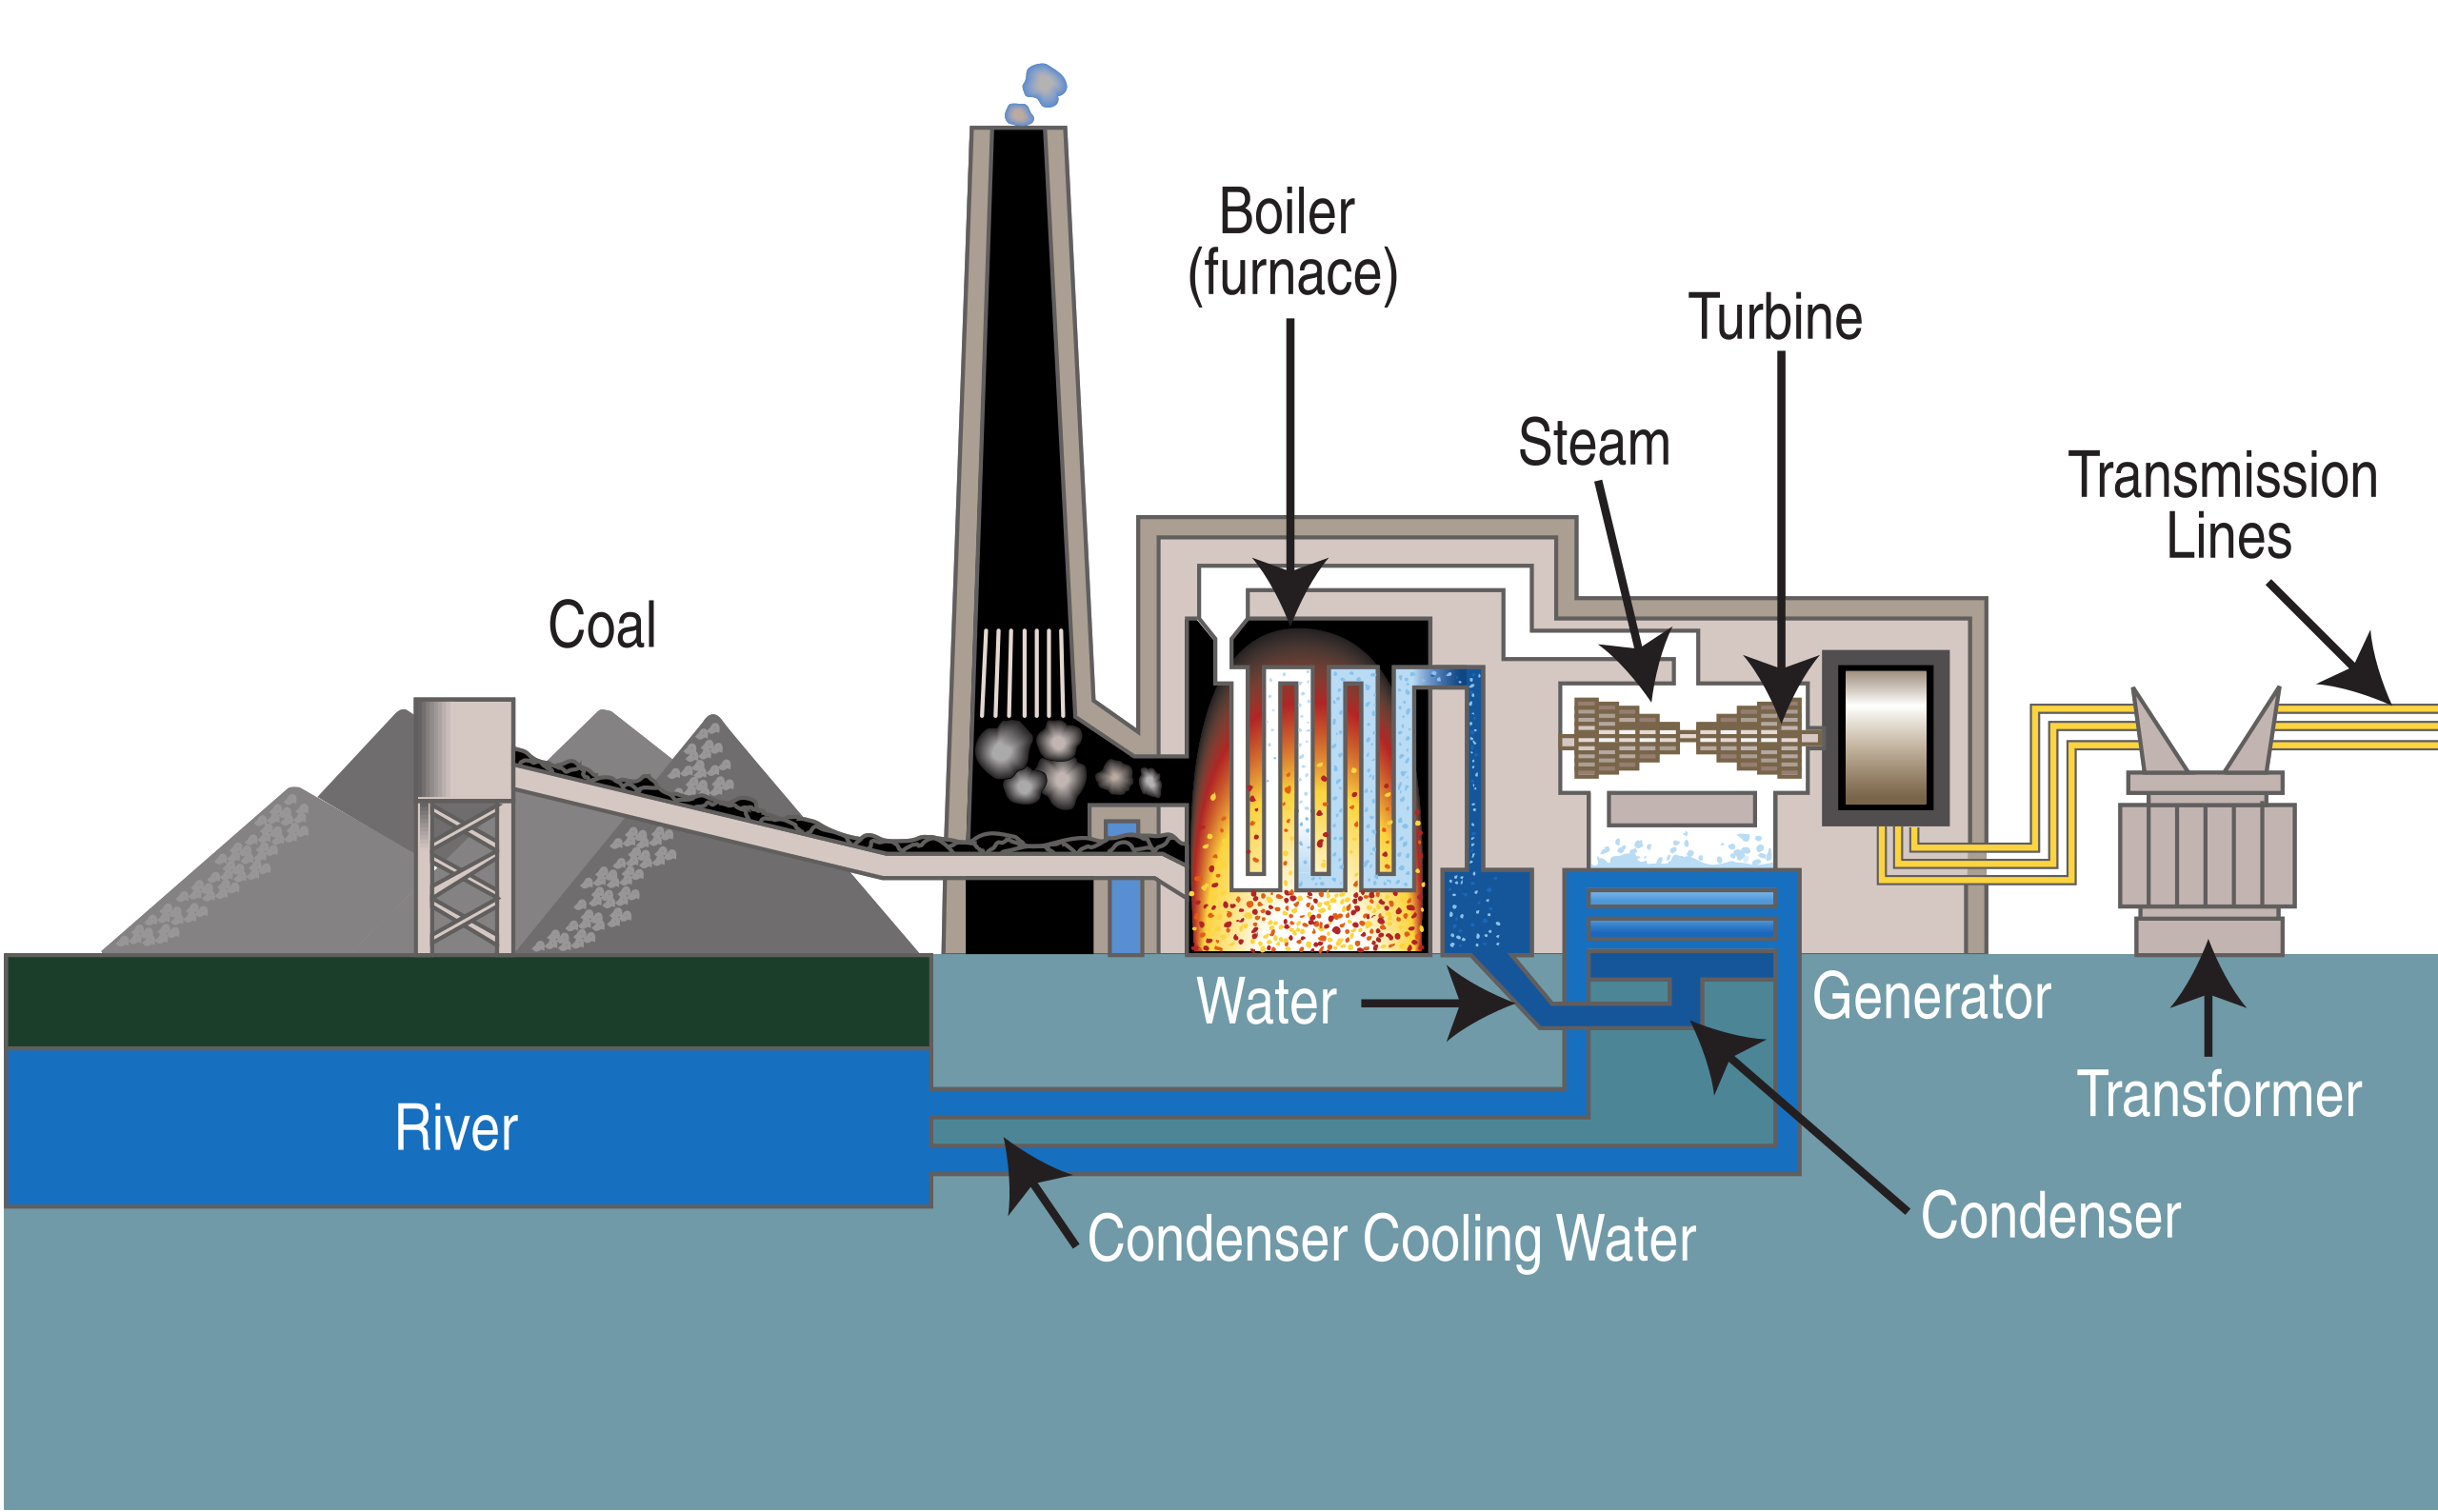
\includegraphics[width=0.7\linewidth]{res/tema10/esquemaFuncional}
	\label{fig:esquemafuncional}
\end{figure}

\section{Circuito aire-combustible-gases-ceniza.}
Este circuito se encarga de:
\begin{itemize}
	\item [-] Recibir y almacenar el combustible.
	\item [-] Preparar el combustible para ser quemado.
	\item [-] Transportar el combustible hasta el hogar.
	\item [-] Evacuación y filtrado de gases.
\end{itemize}
\section{Almacenamiento y preparación del combustible.}
\subsection{Almacenamiento del combustible.}
El almacenamiento se realiza en dos etapas. La primera etapa es el parque de combustible que suele tener una capacidad de almacenamiento de algunos meses de funcionamiento mientras que la segunda se compone por unos depósitos con capacidad para menos de un día.



El carbón se almacena en la cercanía de la central en parques a la intemperie y se maneja mediante rotopalas. Como se debe garantizar que haya un suministro esta la capacidad de almacenamiento suele ser elevada (hasta 150 días). Y si el carbón debe almacenarse más de un año se le proporciona un recubrimiento asfáltico.



No obstante, el almacenamiento de carbón presenta tres problemas principales:
\begin{itemize}
	\item [-] Combustión espontánea: debido al contacto con el aire el carbón se oxida a una velocidad proporcional a la temperatura (se duplica cada 8\grado). A los 65\grado $\ $ empieza a ser peligrosa y por tanto, el apilamiento debe hacerse de manera cuidadosa.
	\item [-] Pérdida de poder calorífica.
	\item [-] Degradación del tamaño del grano.
\end{itemize}


Del parque de almacenamiento se lleva el carbón a una torre de almacenamiento donde se separan las partículas férricas y trozos de piedras que pudiesen dañar los molinos. Tras pasar por la torre el carbón cae a través de las tolvas a unos alimentadores que dosifican la carga a los molinos.
\subsection{Preparación del combustible}
Una parte fundamental de la preparación del combustible consiste en pulverizar el carbón. 



Ventajas de la pulverización:
\begin{itemize}
	\item [-] Rendimiento de la combustión máximo.
	\item [-] Se pueden utilizar carbones de peor calidad.
	\item [-] Las cenizas y escorias no son pastosas (mejor manejo).
	\item [-] Mayor potencia calorífica por unidad de volumen del hogar. 
	\item [-] Menor costo de mano de obra.
 	\item [-] Fácil control del aire y combustible.
\end{itemize}





Desventajas de la pulverización:
\begin{itemize}
	\item [-] Elevado costo inicial de la instalación.
	\item [-] Costo de preparación del combustible.
	\item [-] Posibilidad de crear cenizas volantes (escapen por la chimenea).
\end{itemize}




Además, si el contenido de humedad es muy elevado el carbón antes de entrar al molino se mezcla con gas caliente para evaporar el agua.



Los molinos suelen transformar el carbón desde una granulometría menor a 150 mm hasta un grado de finura de aproximadamente 200$\mu m$ que depende del contenido en volátiles (a mayor contenido en volátiles mayor finura se requiere).



Una vez pulverizado la inyección puede ser:
\begin{itemize}
	\item [-] \textbf{Directa}: el carbón que sale de los molinos se lleva directamente a los quemadores. Es el método \textbf{más utilizado}.
	\item [-] \textbf{Indirecta}: el carbón se hace llegar a los molinos donde es transportado a unos silos de carbón pulverizado donde se almacena hasta que es inyectado en los quemadores.
\end{itemize}
\section{Tipos de molinos.}

\subsection{Molino de anillo de bolas.}
Es un tipo de molino donde un collar de esferas macizas de acero es arrastrado rondado entre dos anillos en los que hay talladas pistas troncotoroidales que guían a las bolas. La presión entre las bolas y anillos se mantiene mediante muelles de acero con una presión regulable.
\begin{figure}[H]
	\centering
	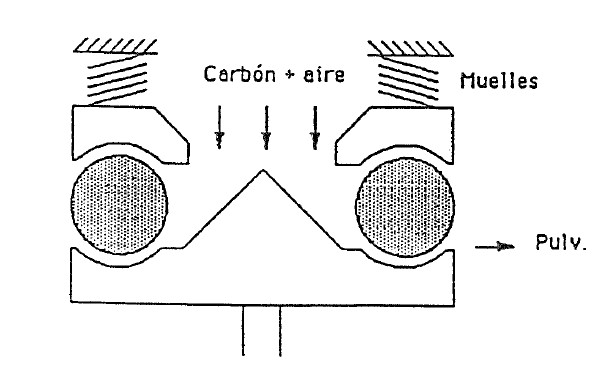
\includegraphics[width=0.4\linewidth]{res/tema10/molinoBolas}
	\label{fig:molinobolas}
\end{figure}

\subsection{Molino tubular de bolas tipo Hardinge.}
Es un molino que consta de un cilindro horizontal con bolas de acero en su interior que gira a velocidad constante. Se emplea aire caliente para secar el carbón y arrastrar el carbón pulverizado a un clasificador espiral.



Como las bolas se van desgastando con el tiempo ne van añadiendo en proporción 0,04-0,23 kg por tonelada de carbón pulverizado. Es un molino adecuado para antracitas aunque es ruidoso y es difícil controlar la finura del polvo. 



Estas calderas suelen absorber de 11 a 30$\frac{kWh}{ton}$ y pueden almacenar grandes cantidades de carbón para seguir suministrando carbón de 6 a 10 minutos.
\begin{figure}[H]
	\centering
	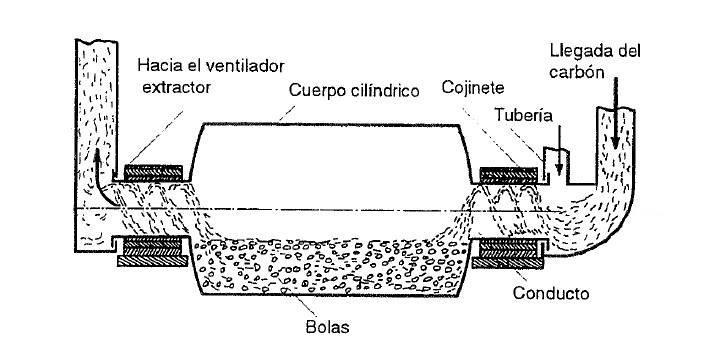
\includegraphics[width=0.6\linewidth]{res/tema10/molinoHardinge}
	\label{fig:molinohardinge}
\end{figure}

\subsection{Molino tubular de bolas Foster Wheeler.}
Es un molino muy simple, adecuado para antracitas. Es ruidoso y de velocidad limitada, pero permite controlar muy bien la finura de polvo. Puede almacenar gran cantidad de carbón.
\begin{figure}[H]
	\centering
	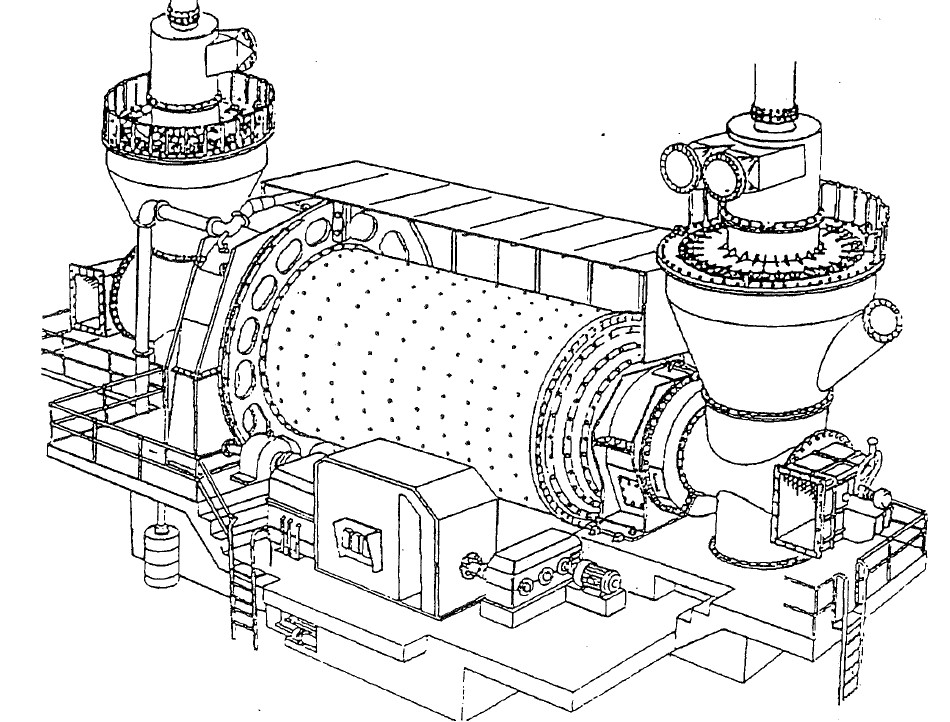
\includegraphics[width=0.4\linewidth]{res/tema10/fosterWheeler}
	\label{fig:fosterwheeler}
\end{figure}

\subsection{Molino de rodillos Babcock-Wilcox.}
Las bolas tienen un diámetro de 51 mm y su velocidad lineal es de 6$\frac{m}{s}$. El consumo de energía es de 8 a 12$\frac{kWh}{ton}$.
\begin{figure}[H]
	\centering
	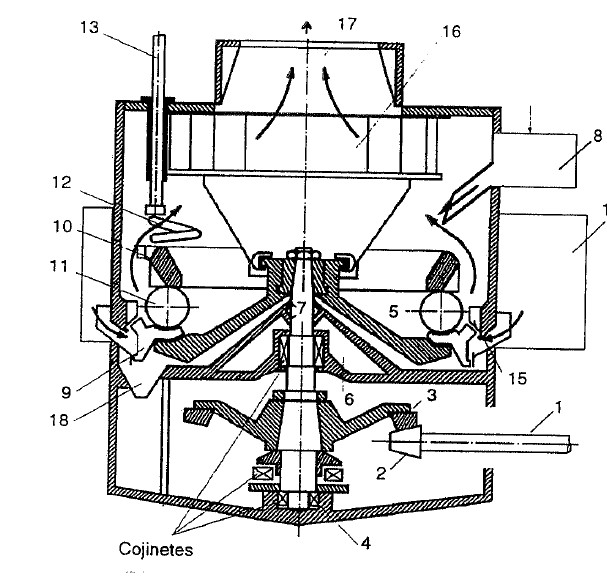
\includegraphics[width=0.3\linewidth]{res/tema10/babcock}
	\label{fig:babcock}
\end{figure}

\subsection{Molino de rodillos de Raymond.}
Este molino consta de tres rodillos que giran sobre un camino de rodadura. La presión correcta se consigue mediante unos muelles ajustables.


Tiene un bajo coste de mantenimiento y es silencioso. Puede triturar 70$\frac{t}{h}$ de carbón pulverizado. Absorbe entre 11 y 16$\frac{kWh}{ton}$.
\begin{figure}[H]
	\centering
	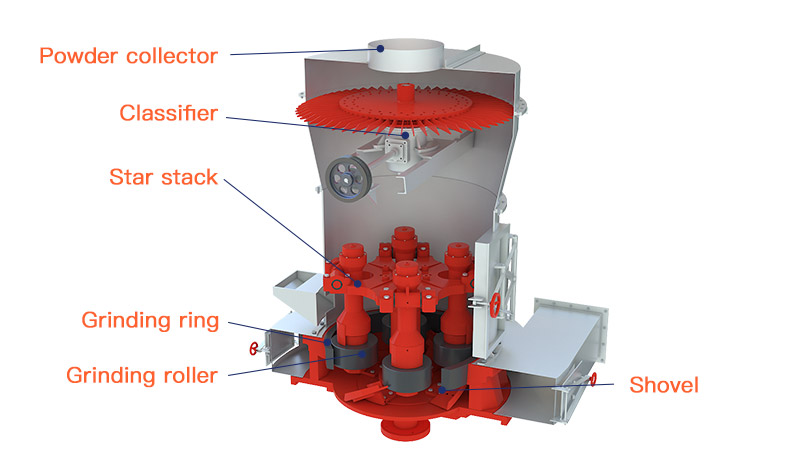
\includegraphics[width=0.5 \linewidth]{res/tema10/raymond}
	\label{fig:raymond}
\end{figure}

\subsection{Molino de batea móvil.}
Es un molino  con una batea móvil con forma troncocónica que gira alrededor de un eje vertical a una velocidad entre 65 y 100 rpm. En su interior se alojan tres muelas cónicas tangentes a la superficie de la batea que giran solidariamente entre sí.




El carbón entra por el centro en el espacio que dejan libres las muelas que a través de la fuerza centrífuga es lanzado contra las paredes donde es triturado por las muelas.


Para extraer este carbón, se emplea aire precalentado que arrastra el carbón pulverizado hacia un separador y las partículas gruesas vuelven al molino.


Este molino tiene bajo costo de mantenimiento y bajo consumo de energía.

\begin{figure}[H]
	\centering
	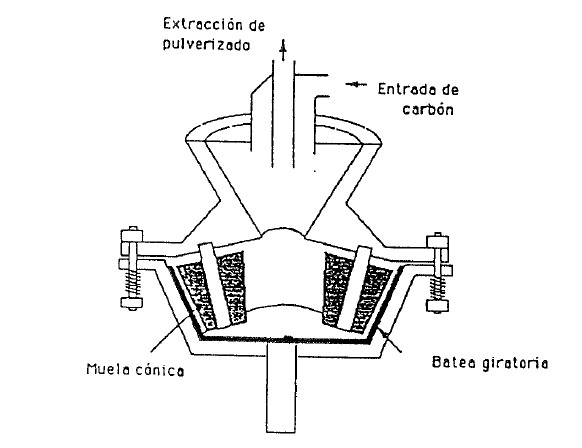
\includegraphics[width=0.5\linewidth]{res/tema10/bateaMovil}
	\label{fig:bateamovil}
\end{figure}


\subsection{Molinos de tipo impacto.}
Este tipo de molinos emplea anillos cilíndricos que giran a una velocidad entre 1000 y 2000 rpm. Dos de los anillos son trituradores y otros dos son lisos para arrastrar el carbón.


A diferencia de anteriores molinos, el carbón descarga directamente por la parte inferior a través de una parrilla que asegura la granulometría deseada.
\begin{figure}[H]
	\centering
	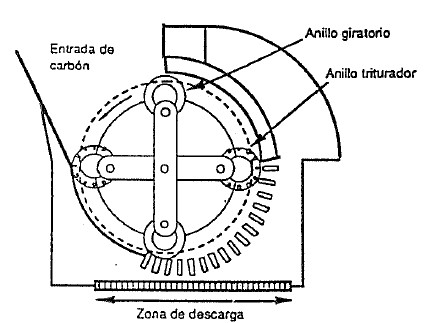
\includegraphics[width=0.5\linewidth]{res/tema10/impacto}
	\label{fig:impacto}
\end{figure}

\section{Circuito aire-gases.}
El aire tomado de la atmósfera se envía mediante ventiladores de tiro forzado a través de precalentadores.

El objetivo de los quemadores:
\begin{itemize}
	\item [-] Recuperar el calor contenido en los gases a la salida de los intercambiadores de agua y vapor.
	\item [-] Elevar la temperatura del aire empleado en la combustión para mejorarla y, para secar el carbón.
\end{itemize}


A la salida de los precalentadores, el aire se envía a la cámara de combustión de diferentes manera:
\begin{itemize}
	\item [-] A través de los quemadores como aire primario mezclado con el combustible.
	\item [-] Alrededor de los quemadores como aire secundario.
	\item [-] A lo largo del recorrido de la llama como aire terciario.
\end{itemize}

\begin{figure}[H]
	\centering
	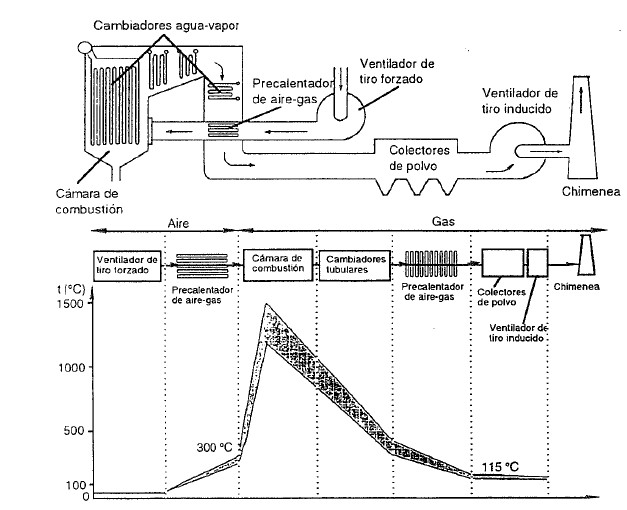
\includegraphics[width=0.7\linewidth]{res/tema10/circuitoAwaGas}
	\label{fig:circuitoawagas}
\end{figure}

\section{Quemadores.}
Los mecheros o quemadores son dispositivos mediante los cuales se introduce carbón pulverizado en suspensión en el aire primario hacia el hogar. Estos dispositivos deben permitir:
\begin{itemize}
	\item [-] El ajuste del punto de ignición.
	\item [-] La estabilidad de la llama (la velocidad de la mezcla aire-carbón iguala a la de propagación de la llama).
	\item [-] La combustión completa.
 	\item [-] La distribución uniforme del exceso de aire y de la temperatura.
	\item [-] El fácil acceso para el mantenimiento.
\end{itemize}



Los quemadores constan de varios conductores donde uno es para el fuel (precalentar el hogar), otro es para el carbón y aire primario y uno adicional para el aire secundario. Además, los quemadores son orientables y se puede modificar su ángulo de incidencia para el control de la combustión.
\begin{figure}[H]
	\centering
	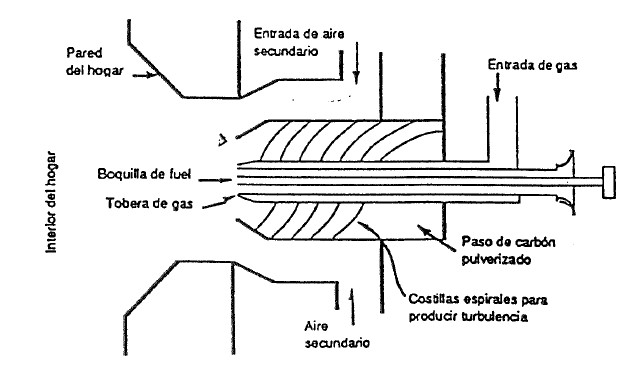
\includegraphics[width=0.6\linewidth]{res/tema10/boquilla}
	\label{fig:boquilla}
\end{figure}


En función del tipo de flujo se tienen:
\begin{itemize}
	\item [-] \textbf{Quemadores de tipo laminar}: las turbulencias se producen por la propia velocidad de la muestra, por el uso de deflectores y por la entrada de aire secundario y terciario.
	\item [-] \textbf{Quemadores de turbulencias}: se imprime un movimiento rotativo al flujo de carbón y aire primario.
\end{itemize}


Para precalentar el hogar de la caldera se emplea combustible líquido (fuel-oil).
\section{Hogar.}
Es la parte de la caldera donde tiene lugar la combustión. El calor desprendido se transmite primero por radiación a todas las partes que están en presencia de la llama y, posteriormente a las partes de la caldera que no ven el fuego mediante convección denominada zona de recuperación de calor (camino de salida de los humos).
\subsection{Pantallas evaporadoras.}
El hogar de una caldera es un volumen diáfano de grandes dimensiones cuyas paredes están
constituidas habitualmente por paneles verticales de tubos soldados de aletas longitudinales
(pantallas evaporadoras). Normalmente van dispuestos verticalmente, soldados a los colectores
extremos (entrada inferior y salida superior).




Por el interior de estos paneles asciende agua de alimentación precalentada a 100\grado $\ $ procedente del economizador, a través de tubos recubiertos de materiales refractarios que bajan desde la parte superior de la caldera (downcommers) que actúa como fluido refrigerante de los propios tubos.


Las paredes de agua van fijas a la envolvente de la caldera de modo que permita su libre
dilatación. 


La envolvente de la caldera es chapa metálica mientras el aislamiento térmico de las paredes
es cemento refractario o roca de vidrio
\section{Ventiladores.}
Para regular la presión en el interior del hogar se emplean ventiladores de tiro forzado que impulsan el aire al interior del hogar para proporcionar presión suficiente para vencer las pérdidas de carga en el circuito aire-gas. No obstante, si la presión en el interior del hogar es menor a la atmosférica (depresión) es necesario un segundo ventilador, de tiro inducido, para aspirar los gases de la combustión y enviarlos a la chimenea.



Las calderas de combustible sólido suelen estar en depresión y las de combustibles líquidos o gaseosos son presurizados.



la geometría de los ventiladores, suele ser de tipo centrífugo donde el aire entra paralelamente al eje y sale de forma radial por medio de una cámara espiral. En estos ventiladores se cumple:
\[Gasto \ másico \propto velocidad\]
\[Presión\propto velocidad^2\]
\[Potencia\propto velocidad^3\]


\subsection{Ventiladores de tiro forzado.}
Se introduce aire a presión al hogar de forma que se vencen los rozamientos y las pérdidas de carga en todo el recorrido de los gases de combustión.
\begin{figure}[H]
	\centering
	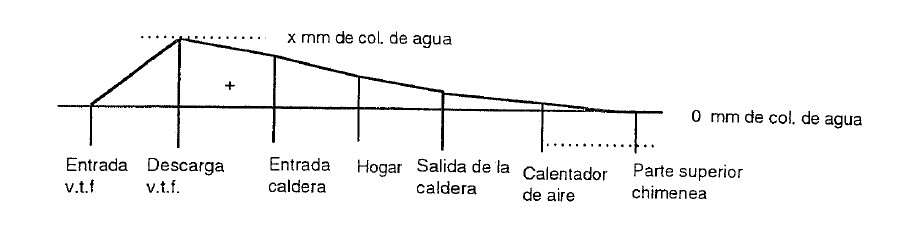
\includegraphics[width=0.7\linewidth]{res/tema10/forzao}
	\label{fig:forzao}
\end{figure}

\subsection{Ventiladores de tiro inducido.}
Se colocan dos por seguridad y se encargan de aspirar los gases del hogar y los envían a la chimenea.
\begin{figure}[H]
	\centering
	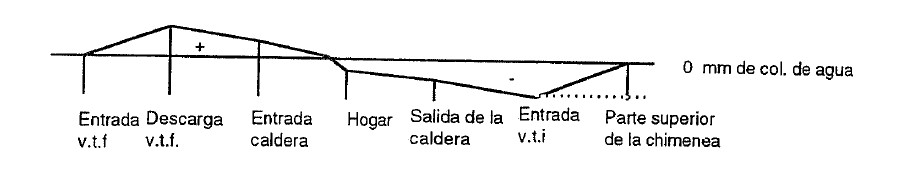
\includegraphics[width=0.7\linewidth]{res/tema10/inducio}
	\label{fig:inducio}
\end{figure}

\section{Precalentadores.}
Su misión es recuperar parte del calor de los gases de combustión para volver a introducirlos en la caldera. De esta forma se aumenta el rendimiento entre un 2,3 y un 2,6\% y un ahorro de combustible entre el 5 y 10\%.



Los precalentadores pueden de tipo:
\begin{itemize}
	\item [-] \textbf{Recuperativo}: los gases y el aire están separados por una pared metálica que transmite el calor.
	\item [-] \textbf{Regenerativo}: la superficie metálica es calentada y enfriada por los gases y el aire de manera alternada. Si tienen un tambor fijo y giran los tubos se denominan de Rothemüle y si el proceso es inverso se denominan de Ljungstrom. 
\end{itemize}
\begin{figure}[H]
	\centering
	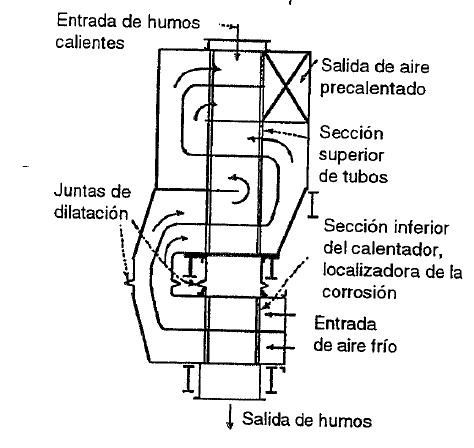
\includegraphics[width=0.4\linewidth]{res/tema10/precalentador}
	\label{fig:precalentador}
\end{figure}



\section{Productos de desecho: Cenizas volantes y escoria.}
El tratamientos para otros productos de desecho de las centrales (gases principalmente) se discutieron en los capítulos 2 y 3. 


Cuando se habla de cenizas volantes y escorias se refiere a compuestos inorgánicos que no se descomponen a la temperatura del hogar pero si se funden. Se diferencia entre las cenizas volantes y la escoria reside en el grosor de estas aglomeraciones. La proporción cenizas volantes y escorias es 4:1 respectivamente.





 Aunque la composición de materia inorgánica varia enormemente según la clase de carbón se pueden establecer los siguientes valores orientativos:
\begin{table}[H]
	\centering
	\renewcommand{\arraystretch}{1.5}
	\begin{tabular}{|c|c|}
		\hline
		Compuesto&$\%$  en peso\\
		\hline
		$SiO_2$&$50,8-32,9$\\
		\hline
		$Al_2O_3$&$30,6-15,1$\\
		\hline
		$Fe_2O_3$&$11,0-32,9$\\
		\hline
		$CaO$&$5,0-8,4$\\
		\hline
		$Na_2O+K_2O$&$2,0-3,0$\\
		\hline
		$MgO$&$0,6-0,8$\\
		\hline
	\end{tabular}
\end{table}



\subsection{Ceniceros.}
Son recipientes diseñados para enfriar las cenizas y evacuarlas al exterior.




En función del tipo de funcionamiento se diferencian entre húmedo y seco. A su vez, los de tipo húmedo se diferencian entre los de funcionamiento continuo (tipo alemán) y funcionamiento intermitente (tipo americano).
\begin{figure}[H]
	\begin{minipage}{0.55\textwidth}
		\centering
		\textbf{Cenicero de tipo alemán.}
		\begin{figure}[H]
			\centering
			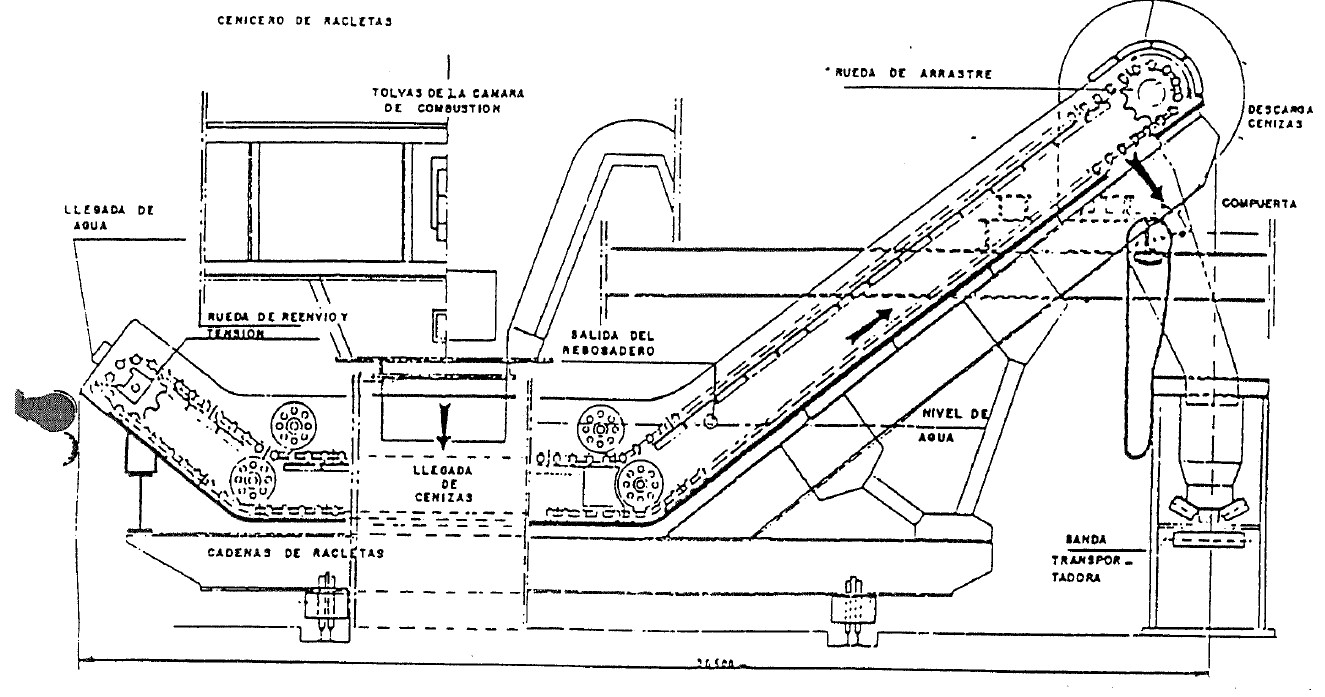
\includegraphics[width=1\linewidth]{res/tema10/aleman}
			\label{fig:aleman}
		\end{figure}
	\end{minipage}
	\begin{minipage}{0.45\textwidth}
		\centering
		\textbf{Cenicero de tipo americano.}
		\begin{figure}[H]
			\centering
			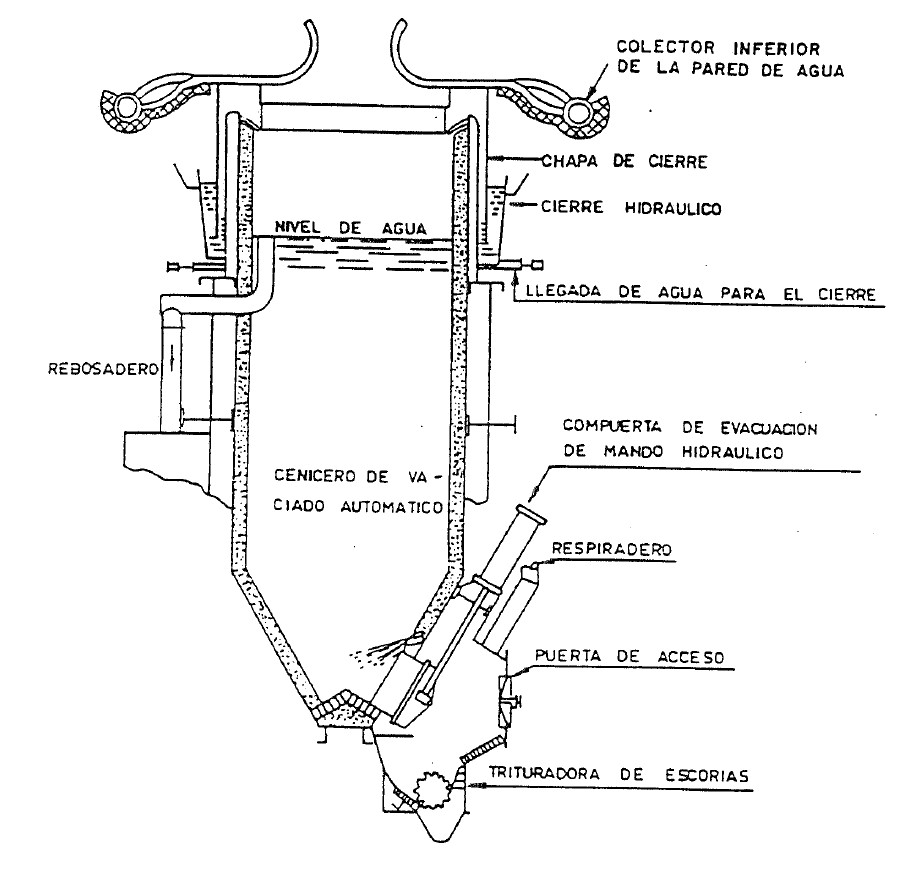
\includegraphics[width=0.7\linewidth]{res/tema10/americano}
			\label{fig:americano}
		\end{figure}
	\end{minipage}
\end{figure}	





\subsection{Retención de cenizas volantes.}
La extracción de de las cenizas volantes se efectúa mediante tolvas colectoras situadas en distintos puntos del circuito aire-gas:
\begin{table}[H]
	\centering
	\renewcommand{\arraystretch}{1.5}
	\begin{tabular}{|c|c|}
		\hline
		Punto&$\%$ de ceniza recogida\\
		\hline
		Precipitador electrostático&$60$\\
		\hline
		Precipitador mecánico&$25$\\
		\hline
		Precalentador de aire&$7$\\
		\hline
		Economizador&$5$\\
		\hline
		Base de la chimenea&$3$\\
		\hline
	\end{tabular}
\end{table}


El principal problema que existe con el contenido en polvo de los gases de combustión es su extremada finura ($50\mu m$). Por ello, para limitar la evacuación de polvo a la atmósfera se emplean filtros mecánicos, electrostáticos o mixtos.
\subsubsection{Filtros mecánicos.}
Separan las partículas más pesadas por cambios de dirección (filtros en zigzag) o por fuerza centrífuga (filtros ciclón). Las partículas intermedias son retenidas por filtros de mangas y las más finas por los electrostáticos.
\begin{figure}[H]
	\begin{minipage}{0.55\textwidth}
El filtrado se puede producir en la masa del material y cuando se colmata hay que sustituirle o bien en su superficie, permitiendo su limpieza. Para ello, se elige recubrir con una capa de Gore-Tex (teflón microporoso).	
\end{minipage}
\begin{minipage}{0.45\textwidth}
\begin{figure}[H]
	\centering
	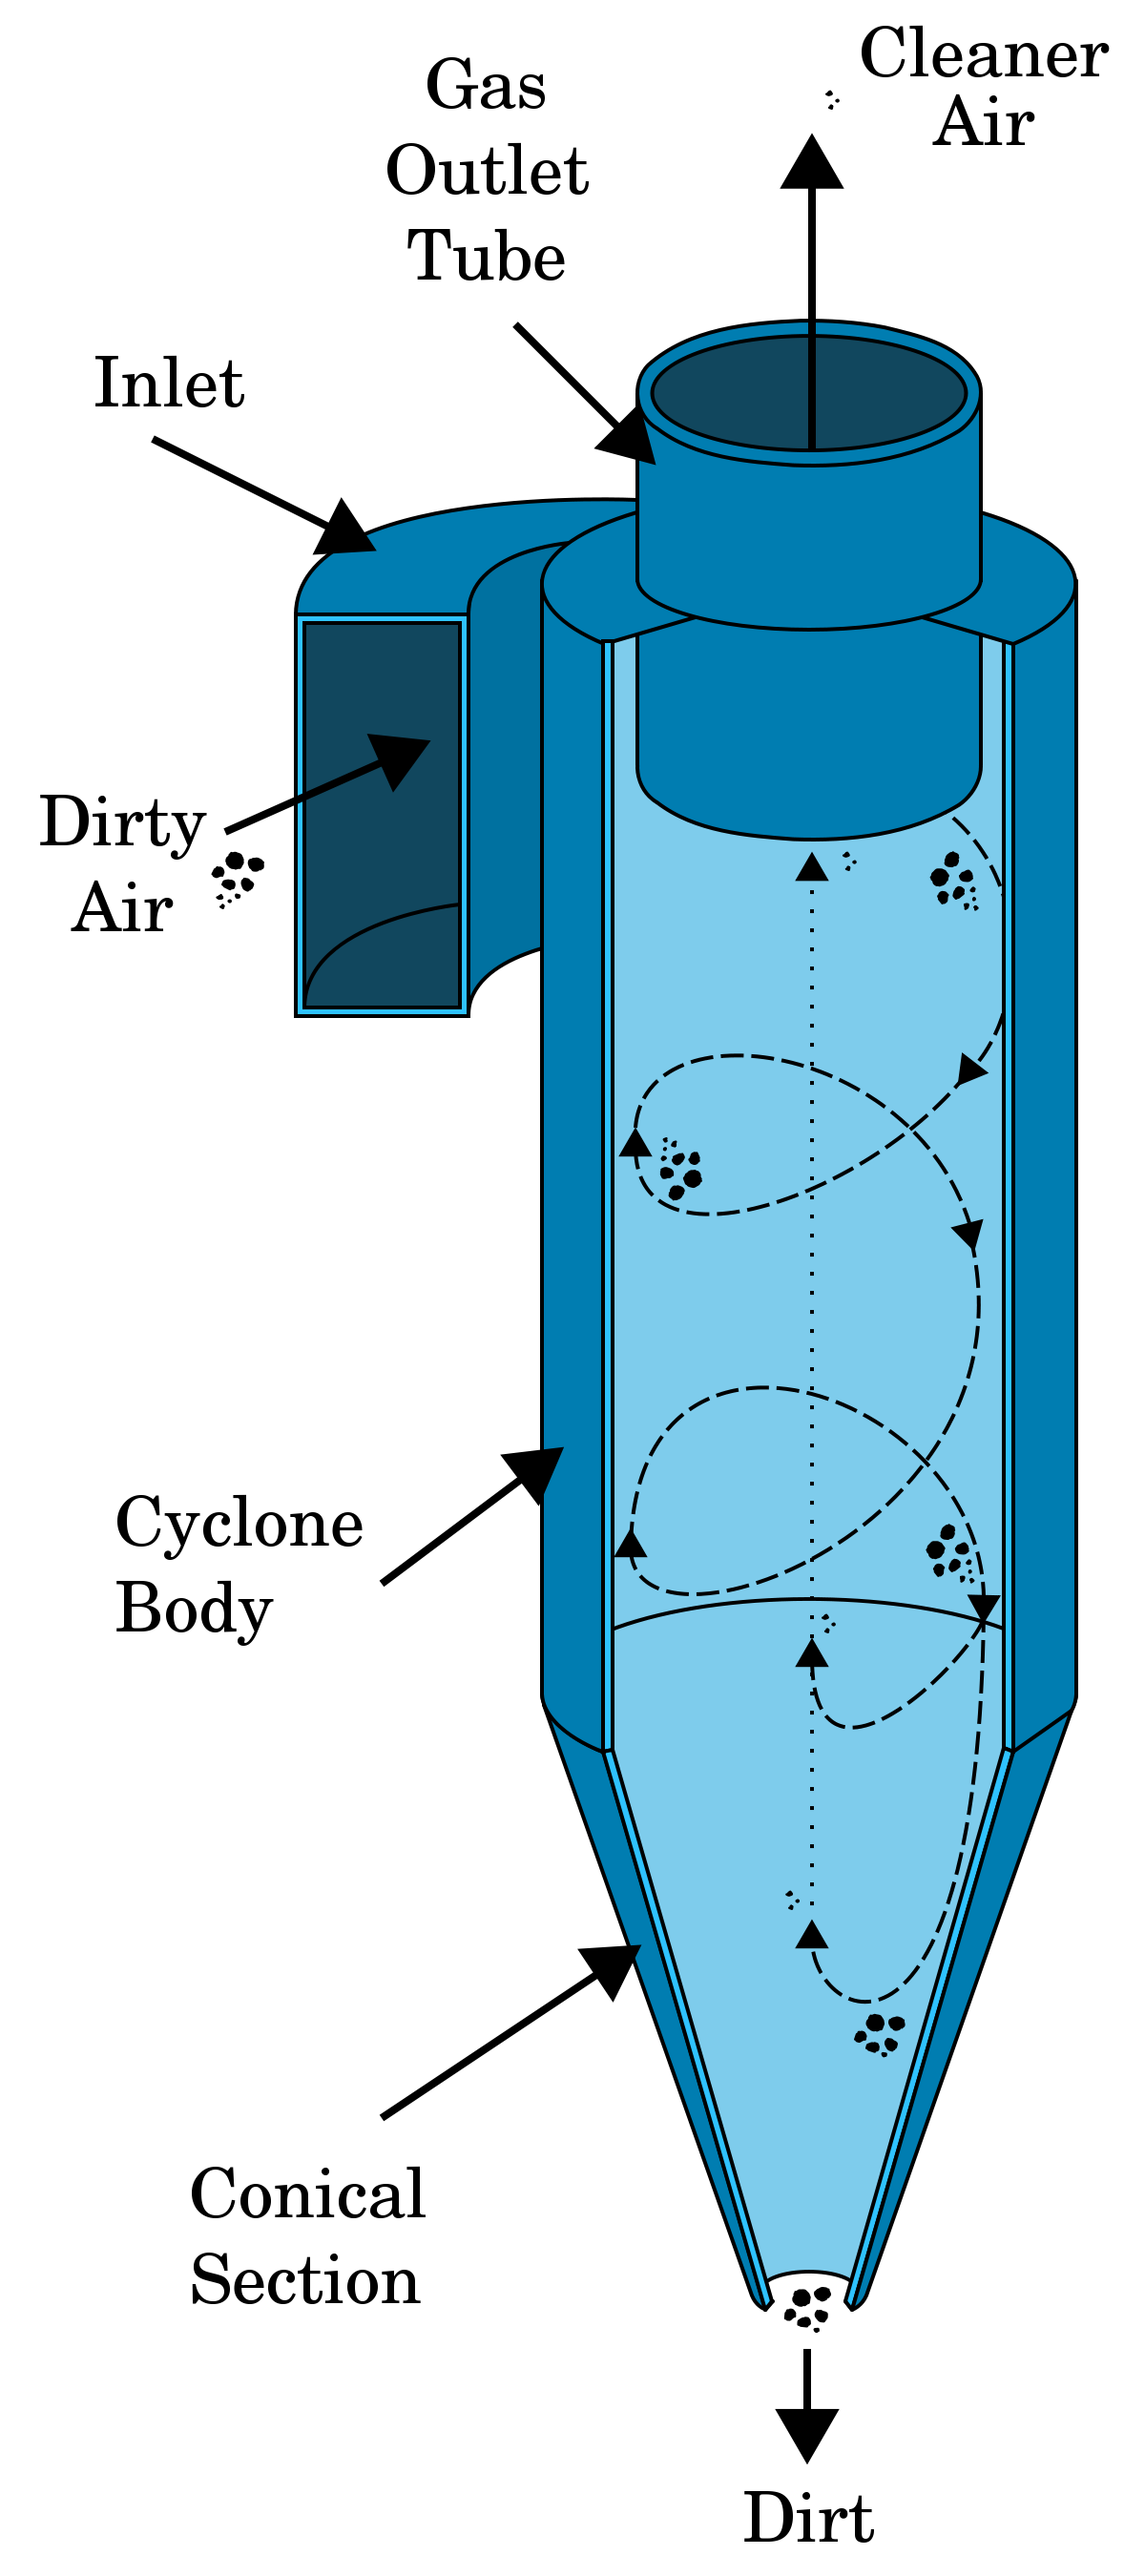
\includegraphics[width=0.4\linewidth]{res/tema10/ciclo9n}

	\label{fig:ciclo9n}
\end{figure}
	\end{minipage}
\end{figure}



\subsubsection{Filtros electrostáticos.}
Se basan en ionizar las partículas mediante un campo eléctrico elevado que posteriormente serán atraídas por los electrodos. Suelen a funcionar entre tensiones de 20 y 100kV y consumir entre 600 y 800kW para una planta de 400MW.
\begin{figure}[H]
	\centering
	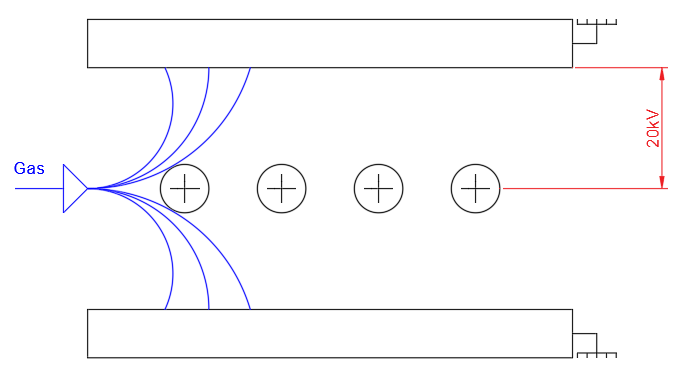
\includegraphics[width=0.7\linewidth]{res/tema2/filtroelectrostatico}
	\label{fig:filtroelectrostatico}
\end{figure} 
\subsubsection{Colectores mixtos.}
Son filtros electromecánicos y utilizan una separación escalonada. A la entrada se coloca el colector mecánico para atrapar las partículas mecánicas y a continuación el electrostático.
\begin{figure}[H]
	\centering
	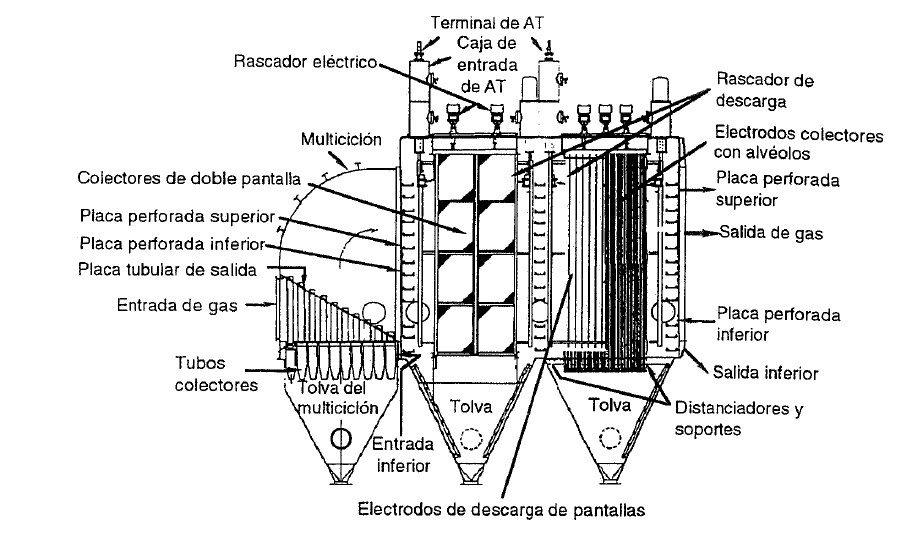
\includegraphics[width=0.7\linewidth]{res/tema10/colectorMixto}
	\label{fig:colectormixto}
\end{figure}

\section{Chimenea.}
Los gases de escape de la combustión, una vez enfriados en los precalentadores hasta cerca de 130 °C
y filtrados en los precipitadores, son aspirados por los ventiladores de tiro inducido y descargados a la
atmósfera por las chimeneas.


La construcción de las chimeneas es de doble pared: la interior con tramos de idéntica sección y
altura, construida con material refractario, y el fuste exterior de hormigón de sección decreciente y
construido en una sola pieza por fraguado continuo.



Las chimeneas son diseñadas para asegurar, en todo momento, que los gases emitidos no van a
afectar la calidad del aire ambiente, a nivel del suelo.

\section{Circuito agua vapor.}
El circuito agua vapor esta compuesto por todos los elementos que participan en el ciclo termodinámico realizado mediante el uso de agua. Este ciclo funciona en circuito cerrado salvo pequeñas pérdidas y desde el punto de vista técnico se suele trabajar a presiones de 180 bar y temperaturas de 550\grado.




Los elementos que forman el circuito son:
\begin{itemize}
	\item [-] Pantallas evaporadoras.
 	\item [-] Sobrecalentador.
 	\begin{itemize}
 		\item Sobrecalentador primario de radiación.
 		\item Sobrecalentador secundario de convección.
 	\end{itemize}
	\item [-] Recalentadores.
	\begin{itemize}
		\item Recalentador primario.
		\item Recalentador secundario.
		\item Recalentador terciario.
	\end{itemize}
	\item [-] Economizador.
	\item [-] Calderín.
	\item [-] Turbina de vapor.
	\begin{itemize}
		\item Cuerpo de alta presión.
		\item Cuerpo de media presión.
		\item Cuerpo de baja presión.
	\end{itemize}
	\item [-] Condensador.
	\item [-] Desgasificador.
	\item [-] Precalentadores de agua de alimentación de la caldera.
	\item [-] Bomba de alimentación agua caldera.
\end{itemize}





\begin{figure}[H]
	\centering
	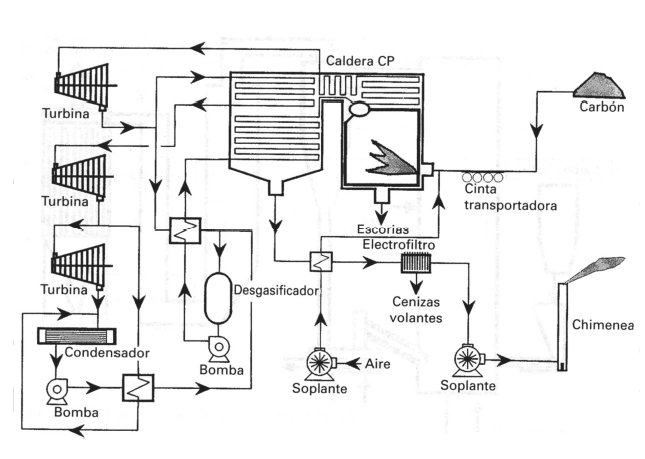
\includegraphics[width=0.7\linewidth]{res/tema10/awaVapor}
	\label{fig:colectormixto}
\end{figure}

\section{Ciclo de Rankine.}
Es el ciclo principal empleado para obtener energía útil a partir del carbón. En las figuras siguientes se puede ver el ciclo básico tanto en diagrama TS como en su ejecución.


\begin{figure}[H]

		
	\begin{minipage}{0.5\textwidth}
		 \begin{adjustbox}{width=1\textwidth}
			\centering
			\begin{circuitikz}
				\tikzstyle{every node}=[font=\normalsize]
				\draw  (3,11.5) circle (0.25cm);
				\draw [short] (2.75,11.5) -- (2.5,11);
				\draw [short] (2.5,11) -- (3.5,11);
				\draw [short] (3.5,11) -- (3.25,11.5);
				\draw [short] (3.25,11.5) -- (5.25,11.5);
				\draw [short] (3,11.75) -- (3,13.25);
				\draw  (5.25,11.75) rectangle (7.25,10.75);
				\draw [short] (7.25,11) -- (9.25,11);
				\draw [short] (9.25,11) -- (9.25,12.75);
				\draw [short] (8.5,13) -- (9.25,12.75);
				\draw [short] (9.25,12.75) -- (10,12.5);
				\draw [short] (10,12.5) -- (10,13.75);
				\draw [short] (8.5,13) -- (8.5,13.5);
				\draw [short] (10,13.75) -- (10,14);
				\draw [short] (8.5,13.5) -- (10,14);
				\draw [short] (9.25,13.75) -- (9.25,15);
				\draw [short] (9.25,15) -- (7.5,15);
				\draw [short] (7.25,15.5) .. controls (7.5,15.25) and (7.5,14.5) .. (7.25,14.5);
				\draw [short] (5.25,14.5) .. controls (5,14.5) and (5,15.25) .. (5.25,15.5);
				\draw [short] (5.25,14.5) -- (7.25,14.5);
				\draw [short] (7.25,15.5) -- (5.25,15.5);
				\draw [short] (5,15) -- (3,15);
				\draw [short] (3,15) -- (3,13);
				\draw [short] (10,13.5) -- (10.75,13.5);
				\draw [short] (10,13) -- (10.75,13);
				\draw  (11.25,13.25) circle (0.5cm) node {\normalsize G} ;
				\draw [->, >=Stealth, dashed] (1.75,11.5) -- (2.75,11.5);
				\draw [->, >=Stealth, dashed] (6.25,10.75) -- (6.25,9.75);
				\draw [->, >=Stealth, dashed] (6.25,16.5) -- (6.25,15.5);
				\draw [->, >=Stealth, dashed] (10.25,14) -- (11.5,14);
				\node [font=\normalsize] at (6.25,16.75) {$Q_C$};
				\node [font=\normalsize] at (6.25,9.5) {$Q_F$};
				\node [font=\normalsize] at (10.5,14.5) {$W_{TV}$};
				\node [font=\normalsize] at (1.75,11.75) {$W_B$};
				\node [font=\normalsize] at (9.25,13.25) {TV};
				\node [font=\normalsize] at (3,11.5) {B};
				\node [font=\normalsize] at (6.25,11.25) {Cond};
				\node [font=\normalsize] at (6.25,15) {Cald};
				\draw [short] (4.25,11.75) -- (4.25,11.25);
				\draw [short] (4.25,14.75) -- (4.25,15.25);
				\draw [short] (8.25,11.25) -- (8.25,10.75);
				\draw [short] (8.25,14.75) -- (8.25,15.25);
				\node [font=\normalsize] at (8.25,15.5) {1};
				\node [font=\normalsize] at (8.25,11.5) {2};
				\node [font=\normalsize] at (4.25,12) {3};
				\node [font=\normalsize] at (4.25,15.5) {4};
			\end{circuitikz}
			\label{fig:my_label}
			 \end{adjustbox}
	\end{minipage}
	\begin{minipage}{0.5\textwidth}
	 \begin{adjustbox}{width=0.8\textwidth}
		\centering	
		\begin{circuitikz}
			\tikzstyle{every node}=[font=\normalsize]
			\draw [->, >=Stealth] (3.5,10) -- (3.5,16.25);
			\draw [->, >=Stealth] (3,10.5) -- (11,10.5);
			\node [font=\normalsize] at (11.25,10.5) {S};
			\node [font=\normalsize] at (3.5,16.5) {T};
			\draw [short] (4.25,11) .. controls (5.25,13) and (5.75,15) .. (6.75,15);
			\draw [short] (6.75,15) .. controls (7.75,14.75) and (8.25,13) .. (10,11.5);
			\draw [->, >=Stealth, dashed] (5.25,13.25) -- (8.5,13.25);
			\draw [->, >=Stealth, dashed] (8.5,13.25) -- (8.5,11.5);
			\draw [->, >=Stealth, dashed] (8.5,11.5) -- (4.5,11.5);
			\draw [->, >=Stealth, dashed] (4.5,11.5) -- (4.5,12.25);
			\draw [->, >=Stealth, dashed] (4.5,12.25) -- (5.25,13.25);
			\node [font=\normalsize] at (8.75,13.5) {1};
			\node [font=\normalsize] at (8.5,11.25) {2};
			\node [font=\normalsize] at (4.5,11) {3};
			\node [font=\normalsize] at (4.25,12.25) {4};
		\end{circuitikz}
		\label{fig:my_label}
	 \end{adjustbox}
	\end{minipage}
\end{figure}
Las distintas etapas del ciclo son:
\begin{itemize}
	\item [-] Proceso 1$\rightarrow$2. Expansión isoentrópica del vapor en la turbina. $\dot{W}_{TV}=h_1-h_2$.
	\item [-] Proceso 2$\rightarrow$3. Condensación isobárica del vapor en el condensador. $\dot{q}_F=h_2-h_3$.
	\item [-] Proceso 3$\rightarrow$4. Compresión isoentrópica en la bomba. $\dot{W}_B=h_4-h_3=\frac{P_4-P_3}{\rho}$.
	\item [-] Proceso 4$\rightarrow$1. Calentamiento isobárico en la caldera. $\dot{q}_C=h_1-h_4$.
\end{itemize}

El rendimiento por otro lado:
\[\eta=\frac{\dot{W}_{TV}-|\dot{W}_B|}{\dot{q}_C}=1-\frac{\dot{q}_F}{\dot{q}_C}\]


En una turbina se cumple que:

\begin{itemize}
	
	

\item [-]La energía mecánica generada por unidad de masa:

\[W=W^*\cdot \eta =(h_1-h_2)\cdot \eta\]
\begin{itemize}
	\item $W$: Trabajo útil por unidad de masa $\left[\frac{kJ}{kg}\right]$.
	\item $W^*$: Trabajo isoentrópico por unidad de masa $\left[\frac{kJ}{kg}\right]$.
	\item $\eta$: Rendimiento mecánico.
	\item $h_1$: Entalpía a la entrada $\left[\frac{kJ}{kg}\right]$.
	\item $h_2$: Entalpía a la salida $\left[\frac{kJ}{kg}\right]$.
\end{itemize}


\item [-]La potencia:
\[P_{mec}=W\cdot \dot{m}\]
\begin{itemize}
	\item $\dot{m}$: Caudal másico de vapor $\left[\frac{kg}{s}\right]$.
\end{itemize}

\end{itemize}

No obstante, este ciclo presenta los siguientes inconvenientes:
\begin{itemize}
  	\item [-] Rendimiento bajo (20-25\%).
	\item [-] El punto 2 del ciclo se sitúa en la región bifásica. Por ello, el vapor tiene un grado de humedad $>10\%$ que provoca un desgaste elevado en los álabes de la turbina.
\end{itemize}



Por ello, para mejorar la eficiencia se pueden tomar las siguientes medidas:
\begin{itemize}
	\item [-] Trabajar a mayor presión en la caldera. 
	\begin{itemize}
		\item Permite aumentar el grado de humedad del vapor de escape.
		\item Se exige una mayor robustez de los elementos lo cual aumenta el coste de la instalación.
	\end{itemize}
	\item [-] Trabajar a mayor temperatura en la caldera.
	\begin{itemize}
		\item Mejora la calidad del vapor a la salida de la turbina.
		\item Mejora el rendimiento interno de la turbina.
		\item  Aumenta el trabajo obtenido en la turbina.
		\item Aumenta el consumo de calor cedido que equivale a mayor consumo de combustible.
	\end{itemize}
	\item [-] Disminuir la presión y temperatura en el condensador.
	\begin{itemize}
		\item Aumenta el trabajo obtenido en la turbina.
		\item Requiere de disponer de agua de refrigeración a la temperatura adecuada.
		\item Como la presión es menor aumenta el volumen ocupado por el vapor. Esto, implica un aumento de las dimensiones de la turbina y condensador.
	\end{itemize}
	\item [-] Sobrecaletar el vapor a la salida de la caldera.
	\begin{itemize}
		\item Disminuye el grado de humedad.
		\item Implica subir la temperatura del punto 4.
	\end{itemize}
	\item [-] Recalentar el vapor a la salida de la turbina.
	\begin{itemize}
		\item Se basa en turbinar en varias etapas. Alta presión, media presión y baja presión.
		\item Se recalienta el vapor a la salida de cada cuerpo. Se lleva el vapor a la caldera.
	\end{itemize}
	\item [-] Precalentar el agua de alimentación mediante extracciones de vapor. 
	\begin{itemize}
		\item Se extrae parte del agua caliente de las turbinas para los calentadores y desgasificador.
	\end{itemize}
\end{itemize}


En el siguiente ciclo, en rojo se marca el sobrecalentamiento y en morado el recalentamiento.
\begin{figure}[H]
	\centering
		\begin{circuitikz}
			\tikzstyle{every node}=[font=\normalsize]
			\draw [->, >=Stealth] (3.5,10) -- (3.5,16.25);
			\draw [->, >=Stealth] (3,10.5) -- (11,10.5);
			\node [font=\normalsize] at (11.25,10.5) {S};
			\node [font=\normalsize] at (3.5,16.5) {T};
			\draw [short] (4.25,11) .. controls (5.25,13) and (5.75,15) .. (6.75,15);
			\draw [short] (6.75,15) .. controls (8,14.75) and (8.25,13) .. (10.25,11.25);
			\draw [->, >=Stealth, dashed] (5.25,13.25) -- (8.5,13.25);
			\draw [->, >=Stealth, dashed] (9.25,14.5) -- (9.25,13.25);
			\draw [->, >=Stealth, dashed] (10,11.5) -- (4.5,11.5);
			\draw [->, >=Stealth, dashed] (4.5,11.5) -- (4.5,12.25);
			\draw [->, >=Stealth, dashed] (4.5,12.25) -- (5.25,13.25);
			\node [font=\normalsize] at (9.25,14.75) {1};
			\node [font=\normalsize] at (10,11) {4};
			\node [font=\normalsize] at (4.5,11) {5};
			\node [font=\normalsize] at (4.25,12.5) {6};
			\draw [ color={rgb,255:red,255; green,0; blue,0}, ->, >=Stealth, dashed] (8.5,13.25) -- (9.25,14.5);
			\draw [ color={rgb,255:red,212; green,0; blue,255}, ->, >=Stealth, dashed] (9.25,13.25) -- (10,14.5);
			\draw [->, >=Stealth, dashed] (10,14.5) -- (10,13.25);
			\draw [ color={rgb,255:red,212; green,0; blue,255}, ->, >=Stealth, dashed] (10,13.25) -- (10.75,14.5);
			\draw [->, >=Stealth, dashed] (10.75,14.5) -- (10.75,12);
			\draw [dashed] (10,11.5) -- (10.75,12);
			\node [font=\normalsize] at (9.25,13) {1'};
			\node [font=\normalsize] at (10,14.75) {2};
			\node [font=\normalsize] at (10,13) {2'};
			\node [font=\normalsize] at (11,14.75) {3};
			\node [font=\normalsize] at (11,12) {3'};
		\end{circuitikz}
	\label{fig:my_label}
\end{figure}

Representando el esquema según sus bloques funcionales.
\begin{figure}[H]
 \begin{adjustbox}{width=0.9\textwidth}
	\centering
		\begin{circuitikz}
			\tikzstyle{every node}=[font=\normalsize]
			\draw [](1.5,15) to[short] (1.5,9.75);
			\draw [](1.5,9.75) to[short] (5,9.75);
			\draw [](5,9.75) to[short] (5,15);
			\draw [short] (5,15) -- (5,15.5);
			\draw [short] (5,15.5) -- (1.5,15.5);
			\draw [short] (1.5,15.5) -- (1.5,14.75);
			\draw [short] (3.25,16.75) -- (3.25,15.5);
			\draw [short] (3,9.75) -- (3,8.75);
			\draw [short] (3,8.75) -- (6,8.75);
			\draw  (6,9.25) rectangle (7,8.25);
			\draw  (8.5,8.75) circle (0.5cm) node {\normalsize $B_{AP}$} ;
			\draw [short] (8,8.75) -- (7.75,8);
			\draw [short] (7.75,8) -- (9.25,8);
			\draw [short] (9,8.75) -- (9.25,8);
			\draw [short] (8,8.75) -- (7,8.75);
			\draw [short] (12,8.75) -- (11,8.75);
			\draw  (10,9.25) rectangle (11,8.25);
			\draw [short] (9,8.75) -- (10,8.75);
			\draw  (13.25,9.25) circle (0.25cm);
			\draw [ fill={rgb,255:red,255; green,255; blue,254} ] (13.25,8.75) ellipse (1.25cm and 0.5cm);
			\node [font=\normalsize] at (13.25,8.75) {Desgasificador};
			\node [font=\normalsize] at (8.5,7.25) {Calentadores};
			\draw [->, >=Stealth, dashed] (9.5,7.25) -- (10.5,8.25);
			\draw [->, >=Stealth, dashed] (7.5,7.25) -- (6.5,8.25);
			\draw [short] (16.5,8.75) -- (16.75,8);
			\draw [short] (15.25,8) -- (16.75,8);
			\node [font=\normalsize] at (15.25,8.5) {};
			\node [font=\normalsize] at (16,8.75) {$B_{AP}$};
			\draw  (16,8.75) circle (0.5cm) node {\normalsize $B_{AP}$} ;
			\draw [short] (15.25,8) -- (15.5,8.75);
			\draw [short] (14.5,8.75) -- (15.5,8.75);
			\draw  (16,11.25) circle (0.5cm) node {\normalsize C} ;
			\draw [short] (16,10.75) -- (16,9.25);
			\draw [short] (3.25,19.25) -- (5.75,19.25);
			\draw (3.25,19) to[R] (3.25,16.75);
			\draw [short] (3.25,19.25) -- (3.25,19);
			\draw [short] (6,17.25) -- (7,17.75);
			\draw [short] (6,17.25) -- (6,16.25);
			\draw [short] (6,16.25) -- (7,15.75);
			\draw [short] (7,15.75) -- (7,17.75);
			\draw [short] (6.5,16) -- (6.5,14.75);
			\draw [short] (6.5,14.75) -- (4.5,14.75);
			\draw [short] (4.5,13) -- (7.75,13);
			\draw [short] (7.75,13) -- (7.75,18.25);
			\draw [short] (5.5,19.25) -- (6.25,19.25);
			\draw [short] (6.5,19.25) -- (6.5,17.5);
			\draw [short] (6,19.25) -- (6.5,19.25);
			\node [font=\LARGE] at (8.5,16.75) {};
			\draw [short] (8.5,17.25) -- (9.5,17.75);
			\node [font=\LARGE] at (9.5,16.75) {};
			\draw [short] (8.5,16.25) -- (9.5,15.75);
			\draw [short] (8.5,17.25) -- (8.5,16.25);
			\draw [short] (9.5,15.75) -- (9.5,17.75);
			\draw [short] (7.75,18.25) -- (9,18.25);
			\draw [short] (9,18.25) -- (9,17.5);
			\draw [short] (9,16) -- (9,12.25);
			\draw [short] (9,12.25) -- (4.5,12.25);		
			\draw (4.5,13) to[R] (4.5,14.75);
			\draw (4.5,10.5) to[R] (4.5,12.25);
			\draw [dashed] (7,17) -- (8.5,17);
			\draw [dashed] (7,16.5) -- (8.5,16.5);
			\draw [dashed] (9.5,17) -- (11,17);
			\draw [dashed] (9.5,16.5) -- (11,16.5);
			\node [font=\LARGE] at (11,16.75) {};
			\draw [short] (11,16.25) -- (12,15.75);
			\node [font=\LARGE] at (12,16.75) {};
			\draw [short] (11,17.25) -- (12,17.75);
			\draw [short] (11,17.25) -- (11,16.25);
			\draw [short] (12,17.75) -- (12,15.75);
			\draw [short] (11.5,16) -- (11.5,13.5);
			\draw [short] (11.5,13.5) -- (16,13.5);
			\draw [short] (16,13.5) -- (16,11.75);
			\draw [short] (4.5,10.5) -- (10.25,10.5);
			\draw [short] (10.25,10.5) -- (10.25,18.25);
			\draw [short] (10.25,18.25) -- (11.5,18.25);
			\draw [short] (11.5,18.25) -- (11.5,17.5);
			\node [font=\normalsize] at (11.5,16.75) {BP};
			\node [font=\normalsize] at (9,16.75) {MP};
			\node [font=\normalsize] at (6.5,16.75) {AP};
			\node [font=\normalsize] at (5,18) {Sobrecalentador};
			\node [font=\normalsize] at (6.25,11.25) {Recalentador 1};
			\node [font=\normalsize] at (3,12.75) {Caldera};
			\node [font=\normalsize] at (6.25,13.75) {Recalentador 2};
			\draw [short] (5.25,9) -- (5.25,8.5);
			\draw [short] (5.25,19.5) -- (5.25,19);
			\draw [short] (6.25,15.25) -- (6.75,15.25);
			\draw [short] (7.5,15.25) -- (8,15.25);
			\draw [short] (8.75,15.25) -- (9.25,15.25);
			\draw [short] (10,15.25) -- (10.5,15.25);
			\draw [short] (11.25,15.25) -- (11.75,15.25);
			\draw [->, >=Stealth] (5.25,8.75) -- (4,8.75);
			\draw [->, >=Stealth] (6.5,18.5) -- (6.5,17.5);
			\draw [->, >=Stealth] (6.5,14.75) -- (5,14.75);
			\draw [->, >=Stealth] (5,13) -- (6.5,13);
			\draw [->, >=Stealth] (6.5,12.25) -- (5,12.25);
			\draw [->, >=Stealth] (5,10.5) -- (6.5,10.5);
			\draw [->, >=Stealth] (16,12.75) -- (16,11.75);
			\draw [->, >=Stealth] (16,10) -- (16,9.25);
			\draw [->, >=Stealth] (15.5,8.75) -- (14.5,8.75);
			\draw [->, >=Stealth] (12,8.75) -- (11,8.75);
			\draw [->, >=Stealth] (10,8.75) -- (9,8.75);
			\draw [->, >=Stealth] (8,8.75) -- (7,8.75);
			\node [font=\normalsize] at (5.25,19.75) {1};
			\node [font=\normalsize] at (6,15.25) {1'};
			\node [font=\normalsize] at (7.25,15.25) {2};
			\node [font=\normalsize] at (8.5,15.25) {2'};
			\node [font=\normalsize] at (9.75,15.25) {3};
			\node [font=\normalsize] at (11,15.25) {3'};
			\node [font=\normalsize] at (5.25,9.25) {6};
			\draw [short] (15.75,10.25) -- (16.25,10.25);
			\node [font=\normalsize] at (15.5,10.25) {5};
		\end{circuitikz}
	\label{fig:my_label}
	\end{adjustbox}
\end{figure}


Por tanto, las ecuaciones teniendo en cuenta extracciones de caudal las expresiones anteriores quedan como:
\[W_{TV}=\dot{m}(h_1-h'_1)+\left(\dot{m}-\dot{m}_e\right)(h'_1-h_2)\]
Donde:
\begin{itemize}
	\item [-] $h'_1$. Entalpía del agua que es extraída de la turbina como agua de alimentación.  
	\item [-] $\dot{m}_e$. Caudal másico extraído de la turbina para la alimentación.
\end{itemize}
\[W_B=\frac{\dot{m}_R\Delta h}{\eta_{bomba}}\]
Donde: 
\begin{itemize}
	\item [-] $\dot{m}_R $. Caudal resultante que circula por la bomba.
\end{itemize}



\subsection{Desviaciones de los ciclos térmicos.}

En los ciclos térmicos reales se producen desviaciones importantes con respecto al comportamiento ideal (denotado con el subíndice s) de
los procesos de expansión en la turbina y de compresión en las bombas debido a que son irreversibles.

\begin{figure}[H]
	\centering
		\begin{circuitikz}
			\tikzstyle{every node}=[font=\normalsize]
			\draw [->, >=Stealth] (3.5,10) -- (3.5,16.25);
			\draw [->, >=Stealth] (3,10.5) -- (11,10.5);
			\node [font=\normalsize] at (11.25,10.5) {S};
			\node [font=\normalsize] at (3.5,16.5) {T};
			\draw [short] (4.25,11) .. controls (5.25,13) and (5.75,15) .. (6.75,15);
			\draw [short] (6.75,15) .. controls (7.75,14.75) and (8.25,13) .. (10,11.5);
			\draw [->, >=Stealth, dashed] (5.25,13.25) -- (8.5,13.25);
			\draw [ color={rgb,255:red,255; green,0; blue,221}, ->, >=Stealth, dashed] (9.25,14.5) -- (9.25,11.5);
			\draw [->, >=Stealth, dashed] (10,11.5) -- (4.5,11.5);
			\draw [ color={rgb,255:red,255; green,0; blue,221}, ->, >=Stealth, dashed] (4.5,11.5) -- (4.5,12.5);
			\draw [->, >=Stealth, dashed] (4.5,12.5) -- (5.25,13.25);
			\node [font=\normalsize] at (9.25,14.75) {1};
			\node [font=\normalsize, color={rgb,255:red,255; green,0; blue,221}] at (9.25,11.25) {2s
			};
			\node [font=\normalsize] at (4.5,11) {3};
			\node [font=\normalsize, color={rgb,255:red,255; green,0; blue,221}] at (4.25,12.75) {4s};
			\draw [->, >=Stealth, dashed] (8.5,13.25) -- (9.25,14.5);
			\draw [->, >=Stealth, dashed] (9.25,14.5) -- (9.75,11.5);
			\node [font=\normalsize] at (9.75,11.25) {2
			};
			\draw [->, >=Stealth, dashed] (4.5,11.5) -- (4.75,12.75);
			\node [font=\normalsize, color={rgb,255:red,54; green,54; blue,54}] at (4.75,13) {4};
		\end{circuitikz}
	\label{fig:my_label}
\end{figure}
\[\eta_{TV}=\frac{h_1-h_2}{h_1-h_{2s}}\]
\[\eta_B=\frac{h_3-h_{4s}}{h_3-h_4}\]


\subsection{Rendimiento de la caldera.}
Recordando expresiones de temas anteriores, se pueden expresar las magnitudes del ciclo de Rankine de la siguiente manera:
\[\eta_{caldera}=\frac{P_{TV}}{P_{carbon}+P_{aire}}\approx\frac{P_{TV}}{P_{carbon}}=\frac{\dot{m}\Delta h}{\dot{m}_{carbon}PCI}\]
\newpage
\subsection{Problema de aplicación.}
\begin{enumerate}
	\item Sea una central que opera con ciclo de Rankine regenerativo con recalentamiento. Rendimiento de las bombas 80\%. Determinar:
	\begin{figure}[h]
		\centering
			\begin{circuitikz}
				\tikzstyle{every node}=[font=\LARGE]
				\draw  (2.25,13.75) rectangle (5.75,9.5);
				\draw [short] (3,9.5) -- (3,8.5);
				\draw [short] (3,8.5) -- (2.25,8.5);
				\draw [short] (2.25,8.5) -- (2.25,7);
				\draw [short] (2.25,7) -- (3.25,7);
				\draw  (3.25,6.75) rectangle  node {\normalsize Calderin} (5.25,7.25);
				\draw  (8.25,6.75) rectangle  node {\normalsize Desgasificador} (10.75,7.25);
				\draw  (11.75,6.75) rectangle  node {\normalsize Calentador baja presion} (15.75,7.25);
				\draw  (16.75,8.5) circle (0.5cm) node {\normalsize $B_{AP}$} ;
				\draw  (6.75,7) circle (0.5cm) node {\normalsize $B_{BP}$} ;
				\draw  (16.75,10.5) circle (0.5cm) node {\normalsize $C$} ;
				\draw  (14.25,12.75) circle (0.5cm) node {\normalsize $G$} ;
				\draw [short] (11.25,13.75) -- (11.25,12.25);
				\draw [short] (11.25,13.75) -- (12.5,13.25);
				\draw [short] (12.5,13.25) -- (12.5,12.25);
				\draw [short] (12.5,12.25) -- (11.25,11.75);
				\draw [short] (11.25,11.75) -- (11.25,12.25);
				\node [font=\normalsize] at (12,12.75) {$AP$};
				\node [font=\normalsize] at (9.5,12.75) {$BP$};
				\draw [short] (10.25,13.75) -- (10.25,11.75);
				\draw [short] (10.25,11.75) -- (9,12.25);
				\draw [short] (9,13.25) -- (10.25,13.75);
				\draw [short] (9,13.25) -- (9,12.25);
				\draw [short] (10.25,13) -- (11.25,13);
				\draw [short] (10.25,12.5) -- (11.25,12.5);
				\draw [short] (12.5,13) -- (13.75,13);
				\draw [short] (12.5,12.5) -- (13.75,12.5);
				\draw [short] (5.25,7) -- (6.25,7);
				\draw [short] (7.25,7) -- (8.25,7);
				\draw [short] (10.75,7) -- (11.75,7);
				\draw [short] (15.75,7) -- (16.75,7);
				\draw [short] (16.75,7) -- (16.75,8);
				\draw [short] (16.75,9) -- (16.75,10);
				\draw [short] (16.75,11) -- (16.75,11.5);
				\draw [short] (16.75,11.5) -- (12,11.5);
				\draw [short] (12,11.5) -- (12,12);
				\draw [short] (4,13.75) -- (4,15.25);
				\draw [short] (4,15.25) -- (9.5,15.25);
				\draw [short] (9.5,15.25) -- (9.5,13.5);
				\draw (5,11.75) to[R] (5,10);
				\draw [](9.5,12) to[short] (9.5,11.75);
				\draw[] (9.5,11.75) to[short] (7,11.75);
				\draw[] (7,11.75) to[short] (5,11.75);
				\draw [short] (5,10) -- (10.75,10);
				\draw [short] (10.75,10) -- (10.75,11.25);
				\draw [short] (10.75,14.75) -- (11.75,14.75);
				\draw [short] (11.75,14.75) -- (12,14.75);
				\draw [short] (12,14.75) -- (12,13.5);
				\draw [dashed] (6.75,10.5) -- (6.75,9.5);
				\draw [short] (6.75,10.5) -- (6.75,11.75);
				\draw [short] (6.75,9.5) -- (6.75,8.5);
				\draw [short] (6.75,8.5) -- (4.5,8.5);
				\draw [short] (4.5,8.5) -- (4.25,8.5);
				\draw [short] (4.25,8.5) -- (4.25,7.25);
				\draw [dashed] (10.75,12) -- (10.75,13.5);
				\draw [short] (10.75,12) -- (10.75,11.25);
				\draw [short] (10.75,13.5) -- (10.75,14.75);
				\draw [short] (11.75,12) -- (11.75,9.25);
				\draw [short] (12,9.25) -- (14,9.25);
				\draw [short] (14,9.25) -- (14,7.25);
				\draw [short] (12,9.25) -- (9.25,9.25);
				\draw [short] (9.25,9.25) -- (9.25,7.25);
				\draw [->, >=Stealth] (3,8.5) -- (3,9.5);
				\draw [->, >=Stealth] (6.25,7) -- (5.25,7);
				\draw [->, >=Stealth] (4.25,8.5) -- (4.25,7.25);
				\draw [->, >=Stealth] (8.25,7) -- (7.25,7);
				\draw [->, >=Stealth] (11.75,7) -- (10.75,7);
				\draw [->, >=Stealth] (16.75,7) -- (15.75,7);
				\draw [->, >=Stealth] (16.75,10) -- (16.75,9);
				\draw [->, >=Stealth] (16.75,11.5) -- (16.75,11);
				\draw [->, >=Stealth] (14,8) -- (14,7.25);
				\draw [->, >=Stealth] (9.25,8) -- (9.25,7.25);
				\draw [->, >=Stealth] (9.5,14.25) -- (9.5,13.5);
				\draw [->, >=Stealth] (12,14.25) -- (12,13.5);
				\draw [->, >=Stealth] (9.5,11.75) -- (5,11.75);
				\draw [->, >=Stealth] (9.25,10) -- (10.75,10);
				\draw [short] (6.75,15.5) -- (6.75,15);
				\draw [short] (8.25,12) -- (8.25,11.5);
				\draw [short] (8.25,10.25) -- (8.25,9.75);
				\draw [short] (5.5,8.75) -- (5.5,8.25);
				\draw [short] (5.75,7.25) -- (5.75,6.75);
				\draw [short] (7.75,7.25) -- (7.75,6.75);
				\draw [short] (11.25,7.25) -- (11.25,6.75);
				\draw [short] (9,8.25) -- (9.5,8.25);
				\draw [short] (13.75,8.25) -- (14.25,8.25);
				\draw [short] (16.25,7.25) -- (16.25,6.75);
				\draw [short] (16.5,9.5) -- (17,9.5);
				\draw [short] (16.25,11.25) -- (16.25,11.75);
				\draw [short] (2,7.75) -- (2.5,7.75);
				\node [font=\normalsize] at (6.75,15.75) {1};
				\node [font=\normalsize] at (8.25,12.25) {2};
				\node [font=\normalsize] at (8.25,10.5) {3};
				\node [font=\normalsize] at (16.25,12) {4};
				\node [font=\normalsize] at (16.25,9.5) {5};
				\node [font=\normalsize] at (16.25,7.5) {6};
				\node [font=\normalsize] at (11.25,7.5) {7};
				\node [font=\normalsize] at (7.75,7.5) {8};
				\node [font=\normalsize] at (5.75,7.5) {9};
				\node [font=\normalsize] at (1.75,7.75) {10};
				\node [font=\normalsize] at (5.5,9) {11};
				\node [font=\normalsize] at (8.75,8.25) {12};
				\node [font=\normalsize] at (13.5,8.25) {13};
			\end{circuitikz}
		\label{fig:my_label}
	\end{figure}
	
	\begin{table}[H]
		\centering
		\renewcommand{\arraystretch}{1.5}
		\begin{tabular}{ccccc}
			\hline
			&P(bar)&T(\grado)&h($\frac{kJ}{kg}$)&Caudal($\frac{kg}{s}$)\\
			\hline
			1&180&540&3390&40\\
			\hline
			2&20&245&2900&40\\
			\hline
			3&20&550&3580&36\\
			\hline
			4&0,04&29&2500&31\\
			\hline
			6&2&¿?&¿?&¿?\\
			\hline
			11&20&245&2900&4\\
			\hline
			12&2&300&3075&1\\
			\hline
			13&0,9&225&2930&1\\
			\hline
		
		\end{tabular}
	\end{table}
	
	\begin{enumerate}
		\item Los valores de P,T, h y caudal en todos los puntos.
		\begin{itemize}
			\item Punto 5 \newline
			Los condensadores trabajan a presión constante. $P_5=P_4=0,04 bar$. Además, la temperatura también es la misma (cambio de estado). $T_5=T_4=29$\grado. Y el caudal también. $\dot{m}_5=31\frac{kg}{s}$. Para calcular la entalpía: $h_5=C_P\cdot T_5=4,18\cdot 29=121,41 \frac{kJ}{kg}$.
			\item Punto 6 \newline
			El caudal másico sigue siendo el mismo. $\dot{m}_6=31\frac{kg}{s}$. Para la entalpía, se emplea el trabajo en la bomba.
			\[|W_{B_{BP}}|=\frac{P_6-P_5}{\rho}=h_6-h_5\rightarrow h_6=h_5+\frac{P_6-P_5}{\rho}=121,41+\frac{(2-0,04)\cdot 10^5}{1000}\cdot 10^{-3}=121,606 \frac{kJ}{kg}\]
			
			
			Para calcular la temperatura:
			\[\Delta h=C_P\cdot\Delta T\rightarrow \Delta T=\frac{\Delta h}{C_P}=\frac{121,606-121,41}{4,18}=0,05^\circ C\]
			\[T_6=T_5+\Delta T=29,05^\circ C\]
			\item Punto 7
			\[\dot{m}_7= \dot{m}_6+\dot{m}_13=31+4=35\frac{kg}{s}\]
			En los calentadores aumenta la temperatura a presión constante.
			\[P_7=P_6=2bar\]
			
			
			En los lugares de convergencia de flujo se cumple:
			\[\sum\left(\dot{m}\cdot h\right)_{entrantes}=\sum\left(\dot{m}\cdot h\right)_{salientes}\rightarrow \dot{m}_7\cdot h_7=\dot{m}_6\cdot h_6+\dot{m}_{13}\cdot h_{13}\]
			\[h_7=\frac{31\cdot121,606+4\cdot2930}{35}=442,57\frac{kJ}{kg}\]
			
			Para calcular la temperatura:
			\[\Delta h=C_P\cdot \Delta T\rightarrow \Delta T=\frac{442,57-121,606}{4,18}=76,79^\circ C\]
			\[T_7=T_6+\Delta T=29,05+76,79=105,83^\circ C\]
			\item Punto 8 \newline
			En la desgasificación se eleva la temperatura a presión constante.
			\[\dot{m}_8=\dot{m}_7+\dot{m}_{12}=35+1=36\frac{kg}{s}\]
			\[P_8=P_7=2bar\]
			\[\dot{m}_8\cdot h_8=\dot{m}_7\cdot h_7+\dot{m}_{12}\cdot h_{12}\rightarrow h_8=\frac{35\cdot442,57+1\cdot3075}{36}=515,69\frac{kJ}{kg}\]
			\[T_8=T_7+\frac{h_8-h_7}{C_P}^=105,83+\frac{515,69-442,57}{4,18}=123,32^\circ C\]
			
			\item Punto 9 \newline
			La presión no varía en el calderín ni en la caldera.
			\[\dot{m}_9=\dot{m}_8=36\frac{kg}{s}\]
			\[P_9=P_1=180bar\]
			\[|W_{B_{AP}}|=h_9-h_8=\frac{P_9-P_8}{\rho}\rightarrow h_9=515,69+\frac{(180-2)\cdot 10^5}{1000}\cdot 10^{-3}=533,49\frac{kJ}{kg}\]
			\[T_9=T_8+\frac{h_9-h_8}{C_P}=132,22+\frac{483,49-515,69}{4,18}=127,48^\circ C\]
			\item Punto 10 \newline
			\[\dot{m}_{10}=\dot{m}_{9}+\dot{m}_{11}=36+4=40\frac{kg}{s}\]
			\[P_{10}=P_1=180bar\]
			\[\dot{m}_{10}\cdot h_{10}=\dot{m}_{9}\cdot h_{9}+\dot{m}_{11}\cdot h_{11}\rightarrow h_{10}=\frac{36\cdot533,49+4\cdot2900}{40}=770,14\frac{kJ}{kg}\]
			\[T_{10}=T_9+\frac{h_{10}-h_9}{C_P}=127,48+\frac{770,14-533,48}{4,18}=184,09^\circ C\]
			
		\end{itemize}
		\item La potencia en la turbina.
		\[W_{AP}=\dot{m}_1(h_1-h_2)=40(3390-2900)=19,6MW\]
		\[W_{BP}=\dot{m}_3(h_3-h_{12})+(\dot{m}_3-\dot{m}_{12})(h_{12}-h_{13})+
		(\dot{m}_3-\dot{m}_{12}-\dot{m}_{13})(h_{13}-h_4)\]
		\[W_{BP}=
		36(3580-3075)+
		35(3075-2930)+
		31(2930-2500)=36,58MW\]
		\[W_{TV}=W_{AP}+W_{BP}=56,16MW\]
		\item La potencia consumida por las bombas.
		\[W_{B_{BP}}=\frac{\dot{m}_5(h_5-h_6)}{\eta_B}=\frac{31(121,41-121,606)}{0,8}=-0,0076MW\]
		\[W_{B_{AP}}=\frac{\dot{m}_8(h_8-h_9)}{\eta_B}=\frac{36(515,69-533,49)}{0,8}=-0,801MW\]
		\[W_B=W_{B_{BP}}+W_{B_{AP}}=-0,8086MW\]
		\item Potencia neta desarrollada por la turbina, la caldera y el condensador.
		\[W_{neto}=W_{TV}-|W_B|=56,18-0,8086=55,3714MW\]
		\[Q_{caldera}=\dot{m}_1(h_1-h_{10})+\dot{m}_3(h_3-h_2)=40(3390-770,14)+36(3580-2900)=129,27MW\]
		\[Q_{condensador}=\dot{m}_4(h_4-h_5)=31(2500-121,41)=73,74MW\]
		\item Rendimiento del ciclo.
		\[\eta=\frac{W_{neto}}{Q_{caldera}}=\frac{55,3714}{129,27}=42,83\%\]
		\[\eta=1-\frac{Q_{condensador}}{Q_{caldera}}=1-\frac{73,74}{129,27}=42,83\%\]
		\item Potencia instalada en barras de la central y del generador si $\eta_{generador}=85\%$, $\eta_{trafo}=98\%$ y $\eta_{autoconsumo}=90\%$.
		\[P_{bg}=W_{neto}\cdot\eta_{generador}=55,3713\cdot0,85=47,06MW\]
		\[P_{bc}=P_{bg}\cdot\eta_{trafo} \cdot \eta_{autoconsumo}=47,06\cdot 0,98 \cdot0,9=41,41MW\]
	\end{enumerate}
\end{enumerate}


\newpage
\section{Caldera acuotubular.}
Para hacer frente a presiones más elevadas, se emplean sistemas de circulación asistida y permiten mayor flexibilidad (periodos de variación de carga). En estos circuitos, se mantiene la circulación en el circuito por medio de bombas de agua instaladas en los tubos bajantes.
\begin{figure}[H]
	\centering
	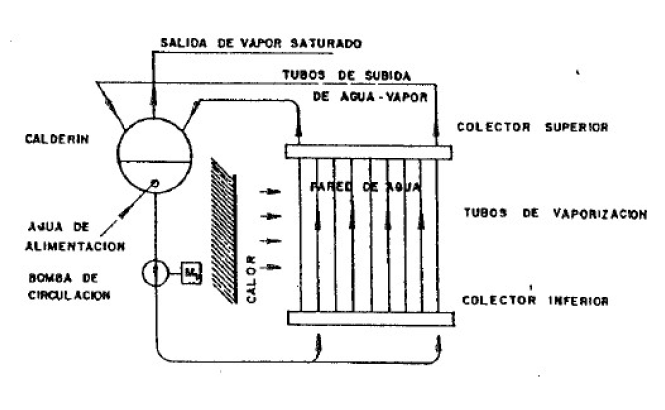
\includegraphics[width=0.7\linewidth]{res/tema10/autotubu}
	\label{fig:autotubu}
\end{figure}



Las calderas de circulación forzada se denominan también generadores de vapor o calderas de circuito abierto. En ellas el agua es impulsada unicamente por una bomba de alta presión (llega a los 230 bar).
\section{Calderín.}
Tiene como objetivo separar las fases líquida y gaseosa por medio de equipos separadores de la mezcla procedente del evaporador para conseguir un vapor seco con grado de humedad $<10\%$. 



El calderín se sitúa en la parte más alta de la caldera y es un gran cilindro horizontal de unos 2 metros de diámetro y 15m de longitud. El cuerpo del calderín se hace de acero especial de manera que soporte las tensiones térmicas (espesor de 10cm):
\begin{itemize}
	\item [-] Interior: 175 bar y 350\grado.
	\item [-] Exterior: 1 bar y 30\grado.
\end{itemize}




El volumen de agua existente en el calderín constituye una gran reserva de
seguridad que amortigua los efectos de los transitorios de carga.



Para realizar el secado del vapor húmedo se centrifuga este mismo de manera que se separa el vapor de la humedad por diferencia de pesos. Tras ello, el vapor seco se pasa el vapor seco a través de chapas apiladas que eliminan el agua residual y llena el pleno gaseoso del calderín. Por otra parte, la humedad pasa a formar parte de la piscina líquida.
\begin{figure}[H]
	\centering
	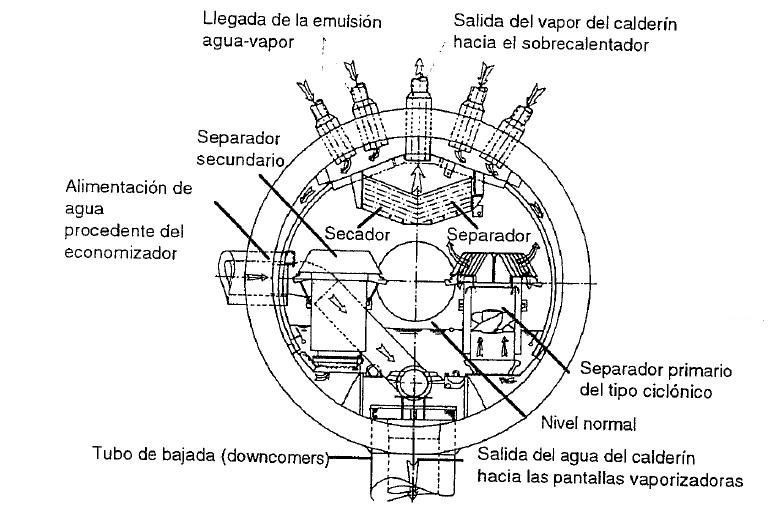
\includegraphics[width=0.7\linewidth]{res/tema10/calderin}
	\label{fig:calderin}
\end{figure}

\section{Sobrecalentadores.}
Son los intercambiadores de haces tubulares que están sometidos a mayores temperaturas,
ya que por su interior circula vapor  y por el
exterior lo hacen los gases de combustión.




Constructivamente, son haces de tubos con diámetros de unos 50mm distribuidos en bancos de profundidad de unos pocos metros y con una ligera separación entre ellos. El vapor circula por su interior a velocidades comprendidas entre 20 y 35 $\frac{m}{s}$.





En función de la temperatura se emplean diferentes materiales. Hasta 540\grado se usan aceros ferríticos de baja aleación (con algo de Cromo, Molibdeno y
Vanadio). Mientras que para temperaturas hasta los 600\grado se sustituyen por aceros austeníticos
(inoxidables, con alto contenido en Cromo 18\% y Níquel 8\%) con un coste notablemente
mayor.




El sobrecalentador se divide en el primario (radiación) y secundario (convección).


\section{Recalentadores.}
En las calderas que alimentan turbinas de dos o tres cuerpos ( alta, media y baja presión)
existen los recalentadores, destinados a recalentar el vapor parcialmente expansionado en el
cuerpo de alta presión.


Los recalentadores tienen características similares a los sobrecalentadores aunque trabajan a aproximadamente una cuarta parte de la presión. Tienen una pérdida de carga de aproximadamente un 4\%.

\section{Economizador.}
Tiene como objetivo reducir el consumo de combustible de la instalación y evitar tensiones térmicas en el calderín. Se sitúa en el extremo final de la zona de recuperación de calor en la caldera.


Es este punto la temperatura de los humos todavía es elevada (por encima de 500\grado) y el
modo predominante de transmisión de calor es por convección.

El economizador es un intercambiador sin mezcla del tipo agua/gas formado por un conjunto de
haces tubulares.

\section{Líneas de vapor.}
Una línea de vapor principal o vapor vivo conduce el vapor sobrecalentado desde la caldera hasta la turbina
de alta presión. La línea de vapor vivo es de gran longitud ya que se extiende desde la parte alta del
edificio de caldera hasta la cota de operaciones en la nave de turbinas.



Una línea de vapor recalentado caliente transporta el vapor ya recalentado hasta la turbina de media presión.



Las tuberías que se emplean para estos circuitos suelen tener diámetros en torno a los 80cm y deben soportar las máximas temperaturas de vapor. Además, se envuelven en aislante térmico para reducir las pérdidas en las tuberías.

\begin{table}[H]
	\centering
	\renewcommand{\arraystretch}{1.5}
	\begin{tabular}{cccc}
		\hline
		Línea&Caudal de vapor ($\frac{t}{h}$)&Presión máxima (bar)&Tª máxima (\grado)\\
		\hline
		Vapor vivo&1900&170&538\\
		\hline
		Vapor recalentado frío&1900&36&421\\
		\hline
		Vapor recalentado caliente&1750&34&538\\
		\hline
	\end{tabular}
\end{table}
\section{Turbinas de vapor.}
La turbina de vapor está destinada a proporcionar potencia mecánica para
mover un generador eléctrico y producir electricidad. Constituye un conjunto denominado
turbogenerador que tiene una velocidad de giro de 1500 o 3000rpm.


El vapor llega a la turbina a alta presión y temperatura (por encima de los 175 bar y 545 \grado) con un alto valor entálpico de 3400$\frac{kJ}{kg}$. De esta forma, durante la expansión, y de forma escalonada según el número de etapas de alabes el vapor transfiere su energía a la turbina generando potencia. 





Si la turbina se compone de más cuerpos la potencia mecánica total es la suma de potencias y si se realizan extracciones l caudal se resta la porción de
vapor extraído.


Debido a la gran longitud que puede alcanzar el turbogrupo ( 20 a 40 m), se divide en tres o
más partes , correspondientes a los cuerpos de la turbina ( alta, media y baja presión) y el alternador. La disposición más común es en eje tamdem-compound , en el que todos los rotores están
alineados en un sólo eje.



Cuantas más etapas tenga una turbina menor será la temperatura de la salida. Sigue la siguiente expresión:
\[\frac{T_ {entrada}}{n_{etapas}}=T_{salida}\]
\subsection{Clasificación de turbinas de vapor.}
Según la dirección del flujo se habla de turbinas axiales o radiales.


Según el tipo de escalonamiento se habla de turbinas tipo Curtis (escalonamiento de velocidad) o de tipo Rateau (escalonamiento de presión). 


\begin{figure}[H]
	\begin{minipage}{0.50\textwidth}
		\centering
		\textbf{Escalonamiento de velocidad.}
		\begin{figure}[H]
			\centering
			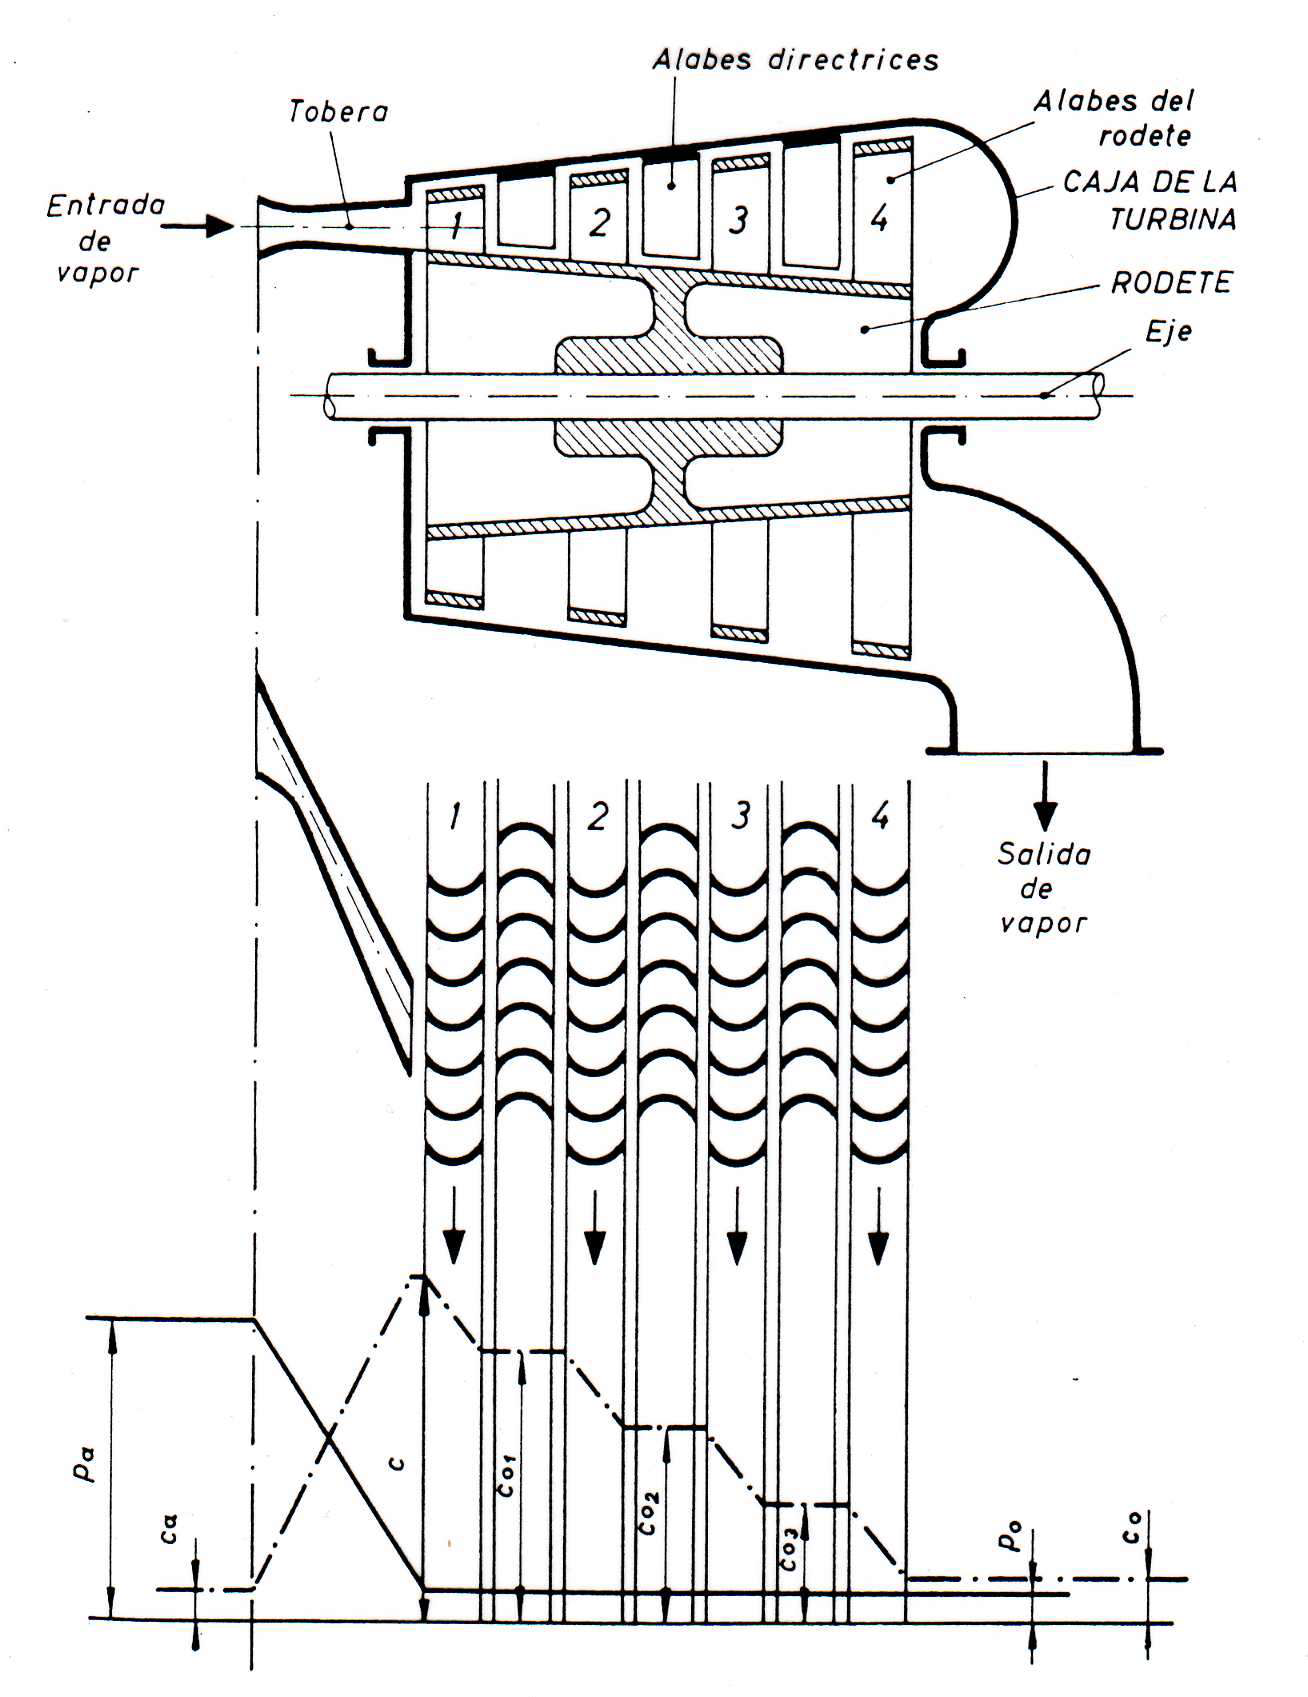
\includegraphics[width=0.7\linewidth]{res/tema10/escVel}
			\label{fig:escvel}
		\end{figure}
	\end{minipage}
	\begin{minipage}{0.50\textwidth}
		\centering
		\textbf{Escalonamiento de presión.}
		\begin{figure}[H]
			\centering
			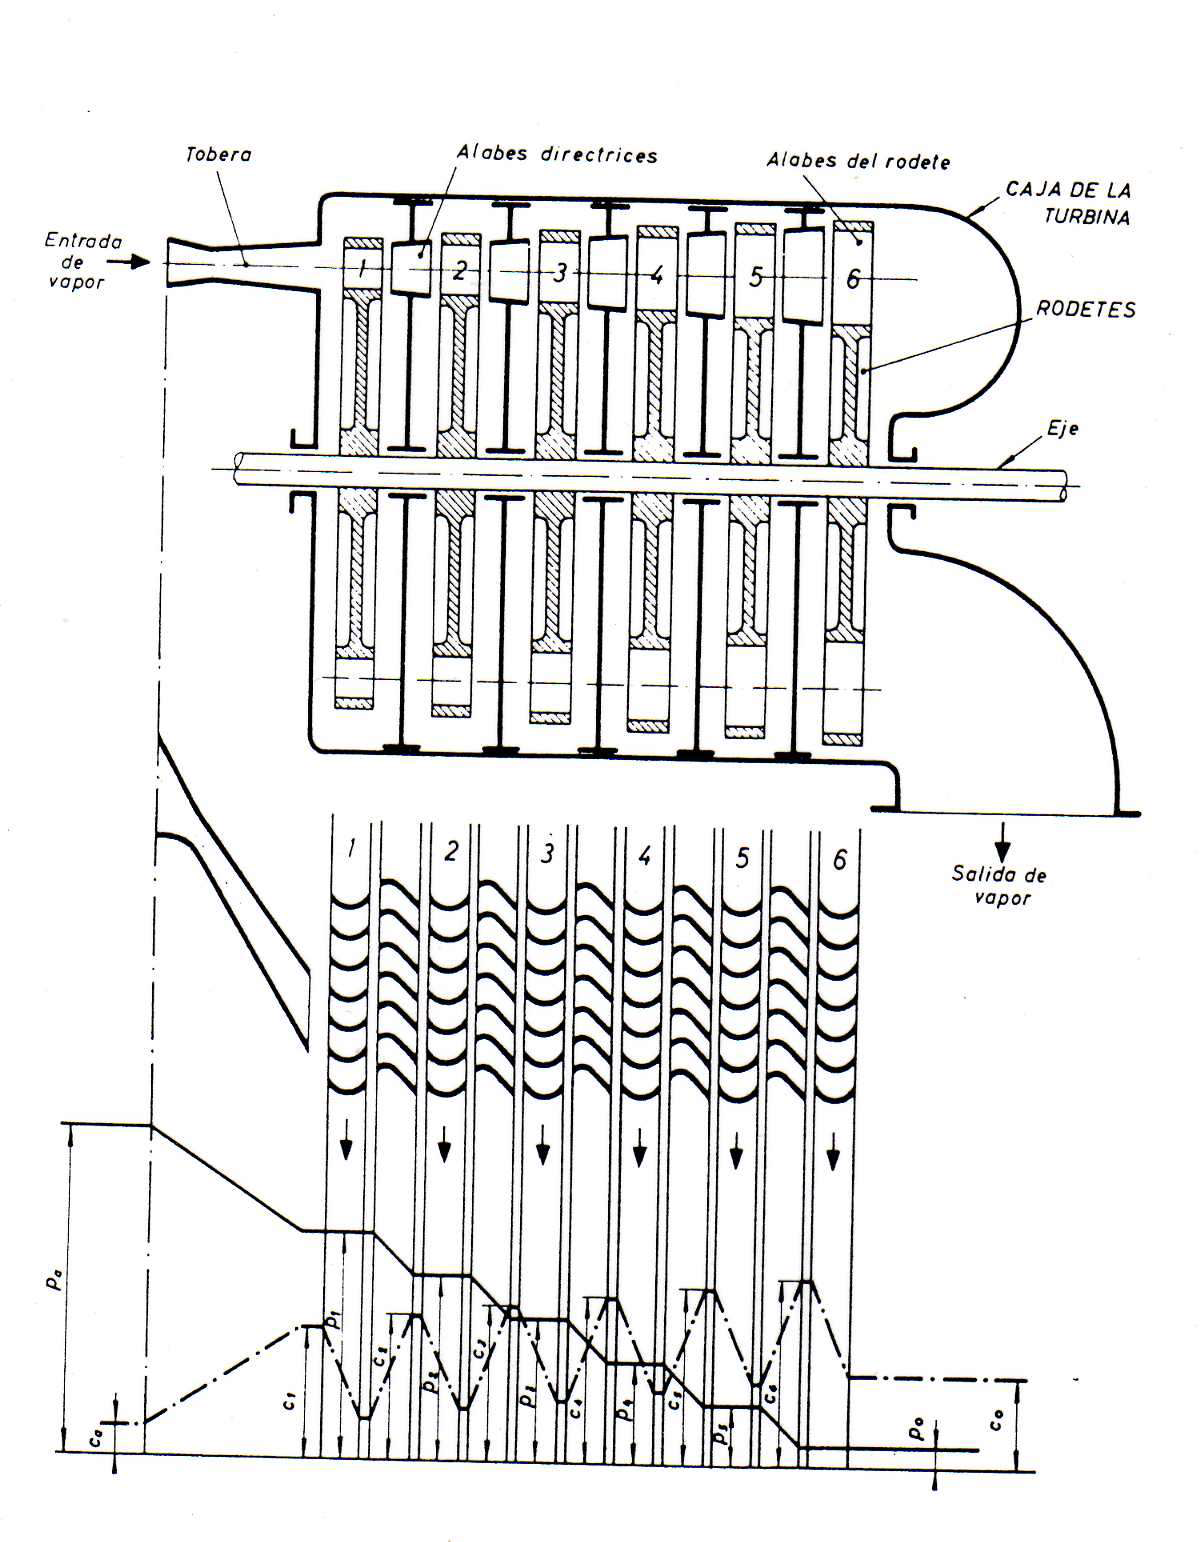
\includegraphics[width=0.7\linewidth]{res/tema10/escpre}
			\label{fig:escpre}
		\end{figure}
	\end{minipage}
\end{figure}








Según el estado del vapor a la entrada de la turbina, puede ser de vapor vivo ( cuerpo de alta presión),
vapor saturado (cuerpo de media presión) o vapor recalentado (cuerpo de baja presión).





\subsection{Recorrido del vapor a través de la turbina.}
El vapor sobrecalentado se conduce a la turbina de alta presión, pasando primero por las válvulas de parada y después por las válvulas de regulación. Tras ello, el vapor pasa por los sucesivos escalonamientos produciendo un trabajo específico
por unidad de masa (salto entálpico). Este vapor sale con una temperatura y presión más baja.


Una vez sale el vapor de la zona de alta presión se recalienta hasta una temperatura similar a la del vapor vivo y, a una presión inferior (50 bar) que será conducida al cuerpo de media presión.

Por último, el vapor expansionado a 10bar se puede introducir en los cuerpos de baja presión simétricos (tubería crossover) o bien ser recalentado.
\section{Condensadores.}
Tiene como función condensar el vapor procedente de la turbina. El calor latente del vapor se transfiere al medio refrigerante para ser disipado a la atmósfera.

Esto supone que, aproximadamente, dos terceras partes del contenido energético del combustible
son evacuadas directamente al condensador.


La temperatura a la que el vapor se condensa depende en gran parte de la temperatura del foco
frío, que no permanece constante en el tiempo. Las variaciones del foco frío pueden ser
estacionales.



Se trata de un equipo esencial, ya que sus condiciones determinan el salto entálpico disponible del
vapor. Para conseguir un máximo de aprovechamiento de la expansión en turbina el condensador trabaja
en condiciones de vacío, a una presión inferior a la atmosférica.


Normalmente, como agente refrigerante, la mayor parte de los condensadores emplean agua.

En función de la disposición de los tubos implicados se habla de intercambiadores de mezcla y de intercambiadores de superficie (más comunes en centrales térmicas).

\begin{itemize}
	\item [-] En los intercambiadores de mezcla existe contacto íntimo entre los fluidos a calentar y condensar.
	\item [-] En los intercambiadores de superficie una barrera física separa ambos fluidos.
\end{itemize}

\subsection{Condensadores de superficie.}
El vapor procedente del
escape de la turbina inunda el vacío de la carcasa , mientras que el agua de refrigeración
fluye por el interior de los tubos con la presión necesaria para vencer las pérdidas de carga.



Como consecuencia del gran volumen específico del vapor a baja presión (20$\frac{m^3}{
	kg}$ a 50
mmHg) y el enorme flujo de vapor a tratar (700 $\frac{t}{h}$ en un grupo de 350 MW ) el tamaño del
condensador es considerable.



El condensador consta de:
\begin{itemize}
	\item [-] Uno o varios cuerpos, generalmente de acero, en los que el vapor es descargado y donde se
	aloja el haz tubular.
	\item [-] Las cajas de agua situadas en los extremos del condensador que sirven para distribuir de
	forma homogénea el caudal del agua de circulación entre todos los tubos.
	\item [-] Haz de tubos , generalmente de aleaciones de cobre, dispuestos verticalmente en forma de
	tresbolillo.
	\item [-] En la zona inferior se ubica una balsa o foso, denominado pozo de condensado o pozo
	caliente, que recoge el vapor ya condensado.
\end{itemize}
\begin{figure}[H]
	\centering
	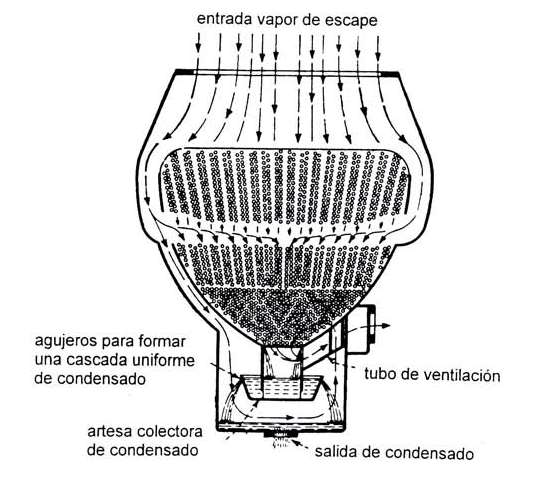
\includegraphics[width=0.7\linewidth]{res/tema10/condensador}
	\label{fig:condensador}
\end{figure}

\section{Sistema de alimentación.}
El vapor condensado se debe bombear nuevamente a la caldera en las condiciones adecuadas de presión y temperatura.



Este bombeo en fase líquida se realiza normalmente en dos etapas, que dan origen a los
sistemas de agua de condensado (desde el pozo caliente del condensador hasta el
desgasificador) y de agua de alimentación (desde el tanque del desgasificador hasta el
economizador de caldera).
\section{Desgasificador.}
Se encarga de que el agua de alimentación  alcance la temperatura de ebullición correspondiente a la presión de vapor de
extracción de la turbina. Para ello, en el desgasificador se debe garantizar un calentamiento uniforme, la desgasificación y la extracción de incondensables (burbujas en al agua).


El calentamiento del agua de condensado con vapor de caldeo se efectúa en diferentes
etapas de acuerdo con el número de extracciones de turbina ya que el rendimiento del ciclo aumenta al emplear el vapor de turbina para calentar el agua del
ciclo.



Las líneas del sistema de extracciones de vapor, que conducen este hasta los calentadores,
van provistas de válvulas de cierre y válvulas de retención controladas para evitar que se
pudiese revertir el flujo de vapor, lo que podría provocar el embalamiento de la turbina si el
grupo se desacopla de la red.


\section{Calentadores de agua de ciclo.}
Habitualmente son de dos pasos por tubo por lo que las cámaras de entrada y salida están
localizadas en el mismo extremo del cambiador. Las velocidades suelen ser de 3$\frac{m}{s}$.
\begin{figure}[H]
	\centering
	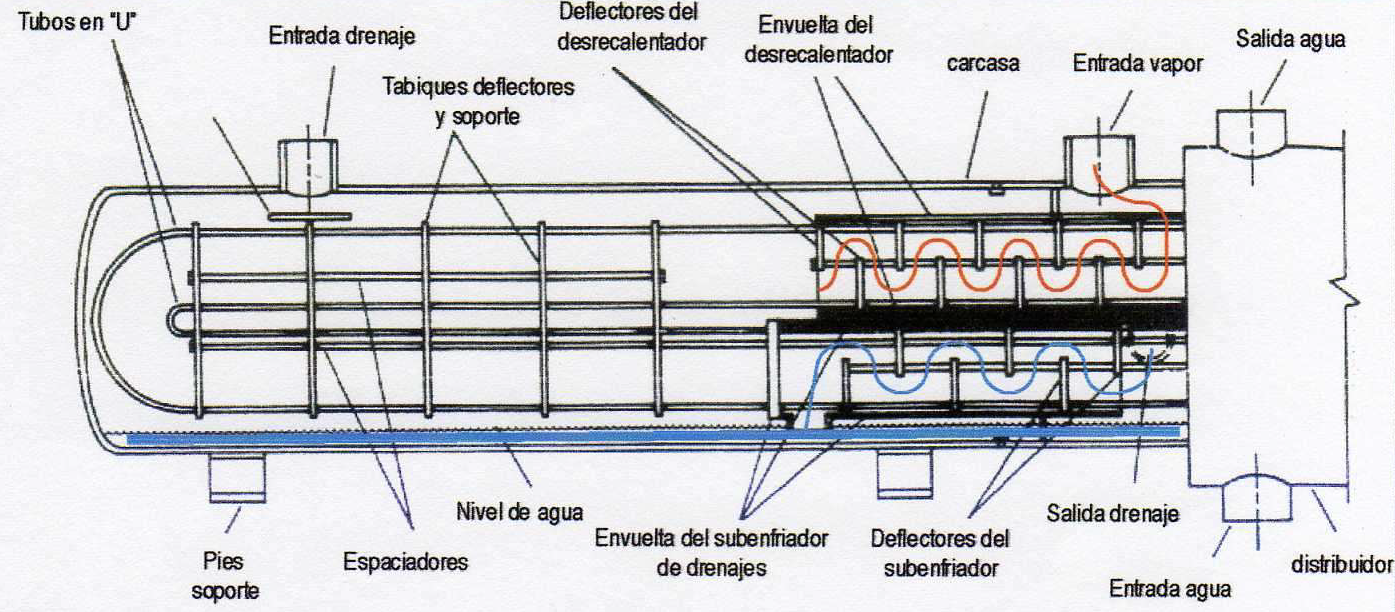
\includegraphics[width=1\linewidth]{res/tema10/calentador}
	\label{fig:calentador}
\end{figure}

Las características geométricas de los cambiadores suelen ser las siguientes:
\begin{table}[H]
	\centering
	\renewcommand{\arraystretch}{1.5}
	\begin{tabular}{cc}
		\hline
		Propiedad&Magnitud\\
		\hline
		Longitud&6-9m\\
		\hline
		Diámetro de la carcasa&0,75-1,5m\\
		\hline
		Número de tubos&400-1200\\
		\hline
		Diámetro tubos&14-146mm\\
		\hline
		Superficie total de calefacción&300-1000$m^2$\\
		\hline
		
	\end{tabular}
\end{table}

\section{Sistema de refrigeración.}
El agua de circulación debe evacuar el calor latente de condensación y, por ello, son necesarios circuitos de refrigeración. Suele provocar que el agia refrigerante tenga una subida de aproximadamente 10\grado.


El sistema de circulación tiene tres disposiciones básicas:
\begin{itemize}
	\item [-] \textbf{Circuito abierto}: el agua se  obtiene aguas arriba de un río y se expulsa aguas abajo.
	\item [-] \textbf{Circuito cerrado}: el agua no sale del circuito y se emplean torres de refrigeración.
	\item [-] \textbf{Circuito mixto}: se obtiene agua aguas abajo de un río y se emplean torres de refrigeración.
\end{itemize}
	
Las bombas de agua están situadas en la toma de agua en un edificio denominado casa de bombas. La toma de aguas debe disponer dispositivos de filtrado adecuados. Las bombas por su parte, suelen ser centrífugas, diseñadas para un gran caudal y tener rendimientos altos.


Por otro lado, las torres de refrigeración son las encargadas del intercambio de materia y energía con el aire ambiente. Por ello, se debe maximizar la cantidad de agua en contacto.


Para ello, el aire asciende por el interior de la torre y el agua desciende por gravedad.


En función de la forma de crear el tiro se distingue entre:
\begin{itemize}
	\item [-] \textbf{Tiro natural}: se basan en la diferencia de densidad entre el aire caliente dentro de la torre y el aire más fresco en el exterior para generar un flujo de aire. Pueden ser hiperbólicas, cilíndricas o troncocónicas.
	\item [-] \textbf{Tiro mecánico}: se basan en el uso de ventiladores para enfriar el agua. Pueden ser de tipo inducido o forzado.
	\item [-] \textbf{Tiro asistido}: es un sistema mixto entre los anteriores.
\end{itemize}

En función del flujo relativo agua-aire:
\begin{itemize}
	\item [-] Flujo en contracorriente.
	\item [-] Flujo cruzado.
\end{itemize}
\section{Tratamiento del agua de alimentación-circuito de refrigeración.}
El agua empleada en una central térmica no debe tener sales e impurezas, pues ello, reduciría considerablemente la vida útil de los distintos componentes del circuito. Por tanto, el agua debe tener las siguientes características:
\begin{table}[H]
	\centering
	\renewcommand{\arraystretch}{1.5}
	\begin{tabular}{ccc}
		\hline
		Elemento/propiedad&Cantidad &Unidades\\
		\hline
		Sólidos disueltos&0,05 &p.p.m\\
		\hline
		Oxígeno disuelto&0,007  &p.p.m\\
		\hline
		Sílice&0,02 &p.p.m\\
		\hline
		Hierro&0,01&p.p.m\\
		\hline
		Cobre& 0,002&p.p.m\\
		\hline
		Dureza&0 &p.p.m\\
		\hline
		$CO_2$&0 &p.p.m\\
		\hline
		Materia orgánica& 0&p.p.m\\
		\hline
		pH&8,5-9,2 & -\\
		\hline
		Conductividad& 20,1&$\frac{\mu s}{cm}$\\
		\hline
	\end{tabular}
\end{table}

Para conseguir estas propiedades se realiza el siguiente proceso de tratamiento:
\begin{enumerate}
	\item Pretratamiento del agua.
	\item Desmineralización del agua pretratada.
	\item Tratamiento del condensado.
	\item Tratamientos adicionales.
	\begin{enumerate}
		\item Clarificación, coagulación y sedimentación.
		\item Ablandamiento.
		\item Esterilización.
		\item Filtración.
	\end{enumerate}
\end{enumerate}




Si no se trata el agua pueden ocurrir las siguientes acciones perjudiciales:
\begin{itemize}
	\item [-] \textbf{Incrustaciones}: son debidas principalmente a los cationes iónicos disueltos. Lo cual produce:
	\begin{itemize}
		\item Disminución del coeficiente de transmisión del calor.
		\item Reducción de la sección útil de las tuberías.
		\item Rotura de tubos por sobrecalentamiento.
	\end{itemize}
	\item [-] \textbf{Corrosiones}: se deben principalmente al oxígeno y en menor medida al dióxido de carbono y otros ácidos minerales. Lo cual produce:
	\begin{itemize}
		\item Disolución del metal de la caldera, economizador, condensador y tuberías.
		\item Los gases insolubles se eliminan en el desgasificador.
		\item El oxígeno residual puede reaccionar con sulfito sódico para dar sulfatos o hidracina para dar agua y nitrógeno libre.
		\item Para contrarrestar la acidificación producida por el dióxido de carbono se inyecta amoniaco. 
	\end{itemize}
\end{itemize}
\section{Control de una central térmica.}
El control de una central térmica se puede realizar siguiendo tres criterios:
\begin{itemize}
	\item [-] \textbf{Turbina siguiendo a caldera}: se utiliza cuando el combustible que se desea gastar no se puede almacenar y se debe consumir a medida que se produce. Centrales que aprovechan el gas de alto horno.
	\item [-] \textbf{Caldera siguiendo a turbina}: es el más extendido y tiene como objetivo satisfacer la demanda eléctrica. 
	\item [-] \textbf{Control coordinado}:
	la señal de demanda de energía actúa simultáneamente sobre caldera y turbina.
\end{itemize}


Los principales controles de una central térmica son:
\begin{itemize}
	\item [-] Control de combustión.
	\item [-] Control de temperatura de vapor sobrecalentado y recalentado.
	\item [-] Control de agua de alimentación.
	\item [-] Control de condensado y drenaje de calentadores.
	\item [-] Control de bypass de alta y baja presión de la turbina.
\end{itemize}

El control de combustión consiste en regular la cantidad de aire y combustible que entran en el hogar, en función de la consigna de potencia eléctrica a suministrar.
\end{document}